\part{The strength and nature of chalcogen bonding}

\begin{refsection}

\chapter[Insights from co-crystal structures]{New insights into chalcogen bonding provided by co-crystal structures of benzisoselenazolinone derivatives and nitrogen bases.}
\label{sec:crystengcomm1}

This chapter was published in Cryst. Eng. Comm., 22 Jan 2019\autocite{Fellowes2019}. \footnote{Compound numbering, section headings, and terminology have been updated to fit this thesis.}

\section{Abstract}
A number of derivatives of benzisoselenazolinones, including the drug ebselen, have been synthesized, and their interactions with various nitrogen bases characterized through x-ray crystallography.
Structural studies revealed a strong interaction in all cases, with Se$\cdots$N distances well within the Van der Waals radii of the constituent atoms.
We suggest that there is a significant charge transfer component to this interaction, in contrast to some other interactions of similar strength and directionality.
We have also found that this interaction can be enhanced via H-bonding to the carbonyl group of the benzisoselenazolinone moiety.

\cmpd*{ebs}
\cmpd*{ebs.bn}
\cmpd*{ebs.h}
\cmpd*{amide}
\cmpd*{amide.bn}
\cmpd*{amide.h}
\cmpd*{tetracycle}

\section{Introduction}
Chalcogen bonding (Ch-bonding) is a class of non-covalent interaction which has recently piqued the interests of the chemical community, and potential applications in materials and medicinal chemistry are emerging.\autocite{Mitchell2017,Wonner2017a,Fanfrlik2014,Vogel2019}
It bears similarities to the related concept of halogen bonding, and the ubiquitous phenomenon of hydrogen bonding, in that the result is a relatively strong and highly directional non-bonded interaction.\autocite{Paolo1974}
This strength and directionality has been exploited in crystal engineering\autocite{Gleiter2003,Kremer2016,Huynh2017}, anion recognition\autocite{Lim2017,Lim2018,Garrett2016}, and bond activation \autocite{Wonner2017,Benz2017,Benz2017a}, and appears to play a critical role in protein folding\autocite{Iwaoka2001,Iwaoka2015}.
Studies on Te$\cdots$N Ch-bonds in solution phase have shown they can be as strong as 2.7~kcal/mol\autocite{Garrett2015a}.
A number of interesting and potentially useful supramolecular polymers have been synthesised and characterised by Vargas-Baca et al., based on tellurium- and selenium-containing heterocycles\autocite{Ho2016,Ho2017}.

In our efforts to apply the concept of Ch-bonding to biological systems, we turned to the benzisoselenazolinone scaffold of the antioxidant compound ebselen \cmpd{ebs}.
\cmpd{ebs} has been known since the 1980s to effectively scavenge reactive oxygen species \emph{in vivo}.\autocite{Muller1984}
It has remarkably low toxicity for an organoselenium compound, and is being investigated as a possible treatment for a number of conditions.\autocite{Schewe1995,Kil2007,Singh2013,Parnham2000}
It is also an ideal scaffold for Ch-bonding, bearing a selenium atom bonded to an electronegative amide nitrogen.
Indeed, Ch-bonding in \cmpd{ebs} has been investigated previously in the context of crystal packing of the pure compound, but there is a lack of experimental evidence for interactions with other acceptors.\autocite{Thomas2015}

Numerous studies have examined the nature of the Ch-bond, in particular the balance between electrostatic effects (due to anisotropic electrostatic potential around the chalcogen atom), covalent (orbital overlap and electron delocalisation), and dispersion forces.\autocite{Oliveira2017,Pascoe2017,DeVleeschouwer2017,Kolar2016,Gleiter2018}
In the case of halogen bonding, these contributions are generally well characterized.
Halogen bonds range from primarily electrostatic (as in the case of fluorinated iodobenzenes\autocite{Prasang2009}) to charge-transfer dominated (molecular halogens\autocite{Mulliken1950}).
In the case of Ch-bonding in derivatives of \cmpd{ebs}, the contributions are less clear.
We therefore sought to characterize Ch-bonding interactions between a number of derivatives of \cmpd{ebs}, and a variety of Ch-bond acceptors.


\section{Results and Discussion}
\subsection[Synthesis of \refcmpd{ebs,ebs.bn,tetracycle}]{Synthesis of benzisoselenazolone derivatives \refcmpd{ebs,ebs.bn,tetracycle}}
Compounds \cmpd{ebs} and \cmpd{ebs.bn} were synthesized via published procedures from amides \cmpd{amide} and \cmpd{amide.bn}.\autocite{Bhabak2010}
The Se-tetracycle \cmpd{tetracycle} was isolated in poor yield as the major product from the cyclization of primary amide \cmpd{amide.h} in an attempt to form \cmpd{ebs.h}.
It is noteworthy that the spectral characteristics of \cmpd{tetracycle} are essentially identical to reported spectral data of \cmpd{ebs.h}\autocite{Bhabak2010}.

\begin{scheme}
  \centering
  \replacecmpd{amide}
  \replacecmpd{amide.bn}
  \replacecmpd{amide.h}
  \replacecmpd{tetracycle}
  \replacecmpd{ebs,ebs.bn}
  \replacecmpd{amide,amide.{bn,h}}
  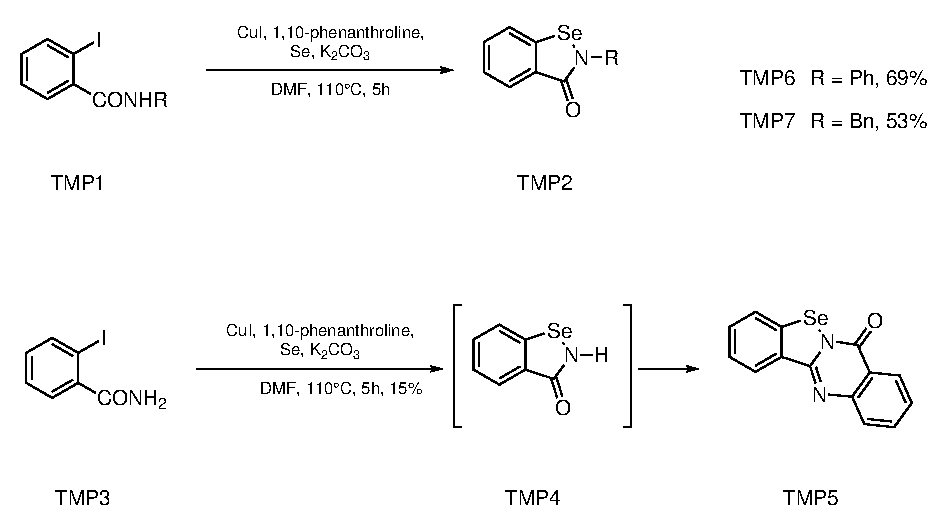
\includegraphics[scale=0.74]{Figures/catalytic-synthesis.eps}
  \caption{Synthesis of Ch-bond donors \refcmpd{ebs}, \refcmpd{ebs.bn} and \refcmpd{tetracycle}.}
  \label{fig:synthesis}
\end{scheme}

\begin{table}
  \centering
  \caption{Selected structural parameters of Ch-bonded complexes.}
  \tablefit{\begin{tabular}{lllllll}
    \toprule
    Complex & r(N$\cdots$Se) & r(Se--N\textsubscript{1}) & r(Se--C\textsubscript{1}) & r(N\textsubscript{1}--C(O)) & $\angle$(N$\cdots$Se--N\textsubscript{1}) & $\angle$(C\textsubscript{para}$\cdots$N$\cdots$Se) \\
      & \AA\ & \AA\ & \AA\ & \AA\ & $^\circ$ & $^\circ$ \\ \midrule
    \cmpd{ebs} only & --- \\
    \cmpd{ebs} $\cdot$ DMAP & 2.371(1) & 1.9676(10) & 1.8959(12) & 1.2345(14) & 174.18(4) & 173.52(4) \\
    \cmpd{ebs.bn} only & --- & 1.8805(14) & 1.8867(16) & 1.350(2) & --- & --- \\
    \cmpd{ebs.bn} $\cdot$ DMAP M1 & 2.4276(14) & 1.9297(13) & 1.8984(15) & 1.348(2) & 173.93(5) & 174.89(5) \\
    \cmpd{ebs.bn} $\cdot$ DMAP M2 & 2.4331(14) & 1.9191(14) & 1.8966(14) & 1.349(2) & 175.30(5) & 158.14(5) \\
    \cmpd{ebs.bn} $\cdot$ DMAP $\cdot$ \ce{H2O} & 2.4046(15) & 1.9367(14) & 1.9070(14) & 1.330(2) & 175.54(5) & 167.43(5) \\
    \cmpd{ebs.bn} $\cdot$ quinuclidine & 2.5874(17) & 1.9077(17) & 1.898(2) & 1.354(3) & 176.77(7) & 161.32(7) \\
    \cmpd{ebs.bn} $\cdot$ DABCO & 2.6166(15) & 1.9019(14) & 1.8967(17) & 1.355(2) & 175.76(6) & 160.00(6) \\
    \cmpd{tetracycle} only & --- & 1.883(2) & 1.899(3) & 1.393(3) & --- & --- \\
    \cmpd{tetracycle} $\cdot$ pyridine & 2.461(3) & 1.926(2) & 1.908(3) & 1.373(4) & 174.13(9) & 169.1(1)\\
    \cmpd{tetracycle} $\cdot$ DMAP & 2.304(1) & 1.9716(9) & 1.918(1) & 1.375(1) & 173.81(4) & 173.16(4) \\
    \bottomrule
    \end{tabular}}
  \label{tab:bondlengths}
\end{table}

\subsection{Co-crystal structures of benzisoselenazolinones and Lewis bases}
High quality low temperature crystal structures were obtained for the parent benzisoselenazolinone derivatives \cmpd{ebs} \autocite{Thomas2015}, \cmpd{ebs.bn} and the Se-tetracycle \cmpd{tetracycle} and the chalcogen-bonded co-crystals of these compounds with a variety of nitrogen bases, including pyridine, dimethylaminopyridine (DMAP), quinuclidine and 1,4-diazabicyclo[2.2.2]octane (DABCO).
Powder diffaction patterns were obtained of the bulk co-crystal material and compared with the single crystal data, with excellent agreement.
This provides strong evidence of phase purity, with the exception of \cmpd{ebs.bn}$\cdot$DMAP, which indicated the presence of the unbound monomers in addition to the Ch-bonded adduct.
Relevant structural parameters are presented in \cref{tab:bondlengths}, while all thermal ellipsoid plots are presented in the supplementary material (\cref{sec:ch3-si}).
In the following discussion we begin by assessing the Ch-bond donor abilities of \cmpd{ebs}, \cmpd{ebs.bn}, and \cmpd{tetracycle} by comparing the structural parameters with a common nitrogen base adduct (DMAP), followed by comparison of a single Ch-bond donor \cmpd{tetracycle} with two different nitrogen bases with markedly different basicities (pyridine and DMAP).

\subsection{Effects of the benzisoselenazolone on Ch-bond strength}
The DMAP adducts of \cmpd{ebs}, \cmpd{ebs.bn} and \cmpd{tetracycle} are characterized by near linear N$\cdots$Se--N(CO) angles (\cref{tab:bondlengths}) with N\textsubscript{DMAP}$\cdots$Se distances which are 2.4276(14) and 2.4331(16)~\AA \ for the two independent molecules of \cmpd{ebs.bn}, 2.371(1)~\AA\ for \cmpd{ebs}, and the strikingly short N$\cdots$Se distance of 2.304(1)~\AA\ for \cmpd{tetracycle}.
All are well within the van der Waals radii of N and Se of 3.85~\AA\ \autocite{Batsanov2001}.
The antipodal Se--N\textsubscript{1} bond distance within these adducts is significantly lengthened compared to the free Ch-bond donors, 0.063~\AA\ in \cmpd{ebs}, 0.049~\AA\ in \cmpd{ebs.bn}, and 0.088~\AA\ in \cmpd{tetracycle}, with the degree of lengthening being related in an inverse sense to the N\textsubscript{DMAP}$\cdots$Se distance, in all cases the (non-antipodal) Se--C\textsubscript{1} bond is essentially unchanged.
These structural parameters suggest an order of Ch-bond donor abilities \cmpd{ebs.bn} < \cmpd{ebs} < \cmpd{tetracycle}, which is supported by theoretical calculations which are discussed below, as well as being consistent with the \textsuperscript{77}Se NMR chemical shifts.

\subsection{Endocyclic bond lengthening associated with stronger complexes}
Further discussion is warranted on the \cmpd{ebs.bn}$\cdot$DMAP adduct.
Firstly, the two independent molecules of \cmpd{ebs.bn}$\cdot$DMAP differ significantly with respect to the direction that the nitrogen base lone pair makes with the Se--N\textsubscript{1} bond.
In molecule 1 this angle is close to colinear at 174.89(5)$^\circ$ while in molecule 2, this deviates significantly from linearity 158.14(5)$^\circ$.
Associated with this difference is a slightly longer N\textsubscript{DMAP}$\cdots$Se distance of 2.4331(14)~\AA\ in molecule 2 compared to 2.4276(14)~\AA\ in molecule 1 ($\Delta$=0.0055~\AA ; 3$\sigma$) and a shorter Se--N\textsubscript{1} distance 1.9191(14)~\AA\ vs 1.9297(14)~\AA\ ($\Delta$=-0.10~\AA ; 7.5$\sigma$) indicating a slightly weaker interaction.
This can be seen in \cref{fig:benzyl-dmap-xray-2}.

\begin{figure}
  \centering
  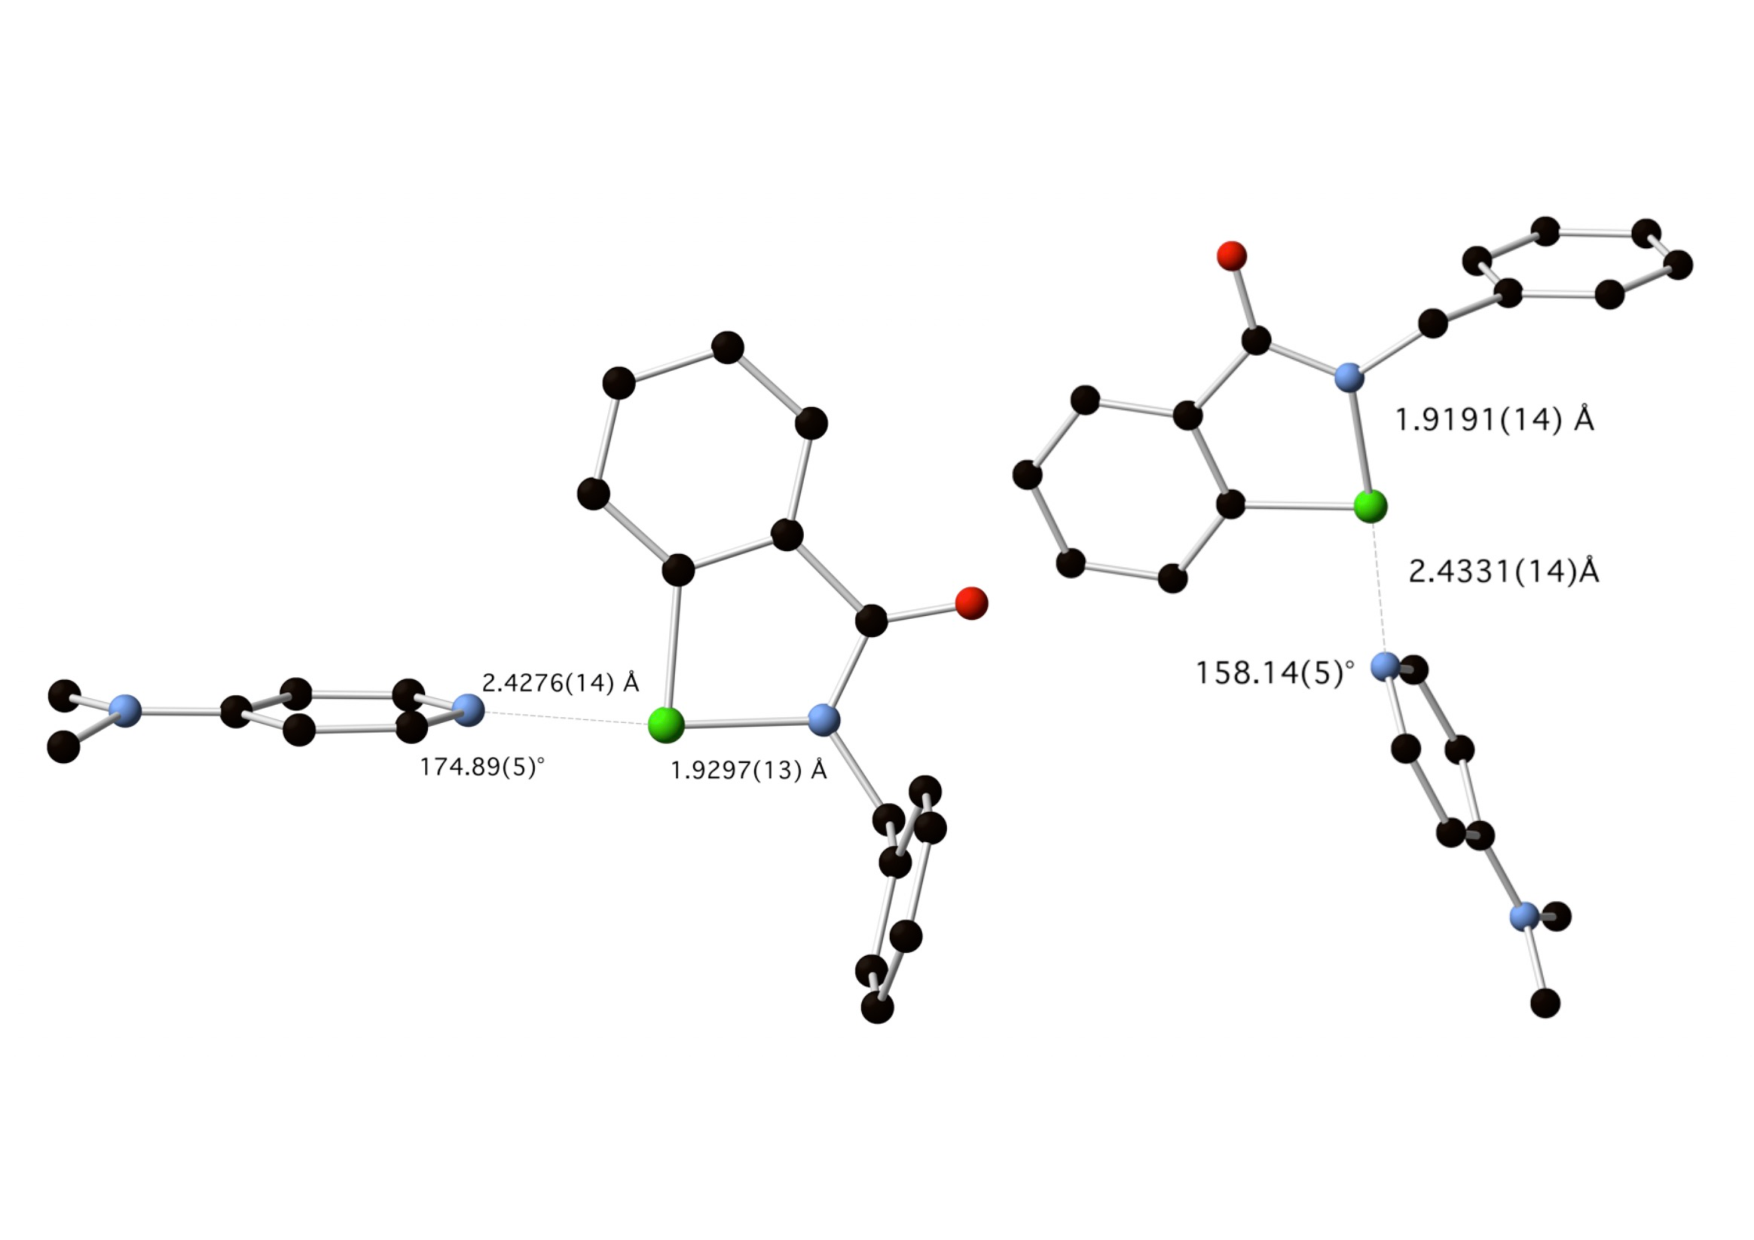
\includegraphics[width=0.8\linewidth]{Figures/benzyl-dmap-xray-2.pdf}
  \caption{Structure of \refcmpd{ebs.bn}$\cdot$DMAP, showing the two distinct geometries.}
  \label{fig:benzyl-dmap-xray-2}
\end{figure}

The structural effects described, particularly the lengthening of the Se--N\textsubscript{1} bond are consistent with donation of electron density from the nitrogen lone pair into the Se--N\textsubscript{1} antibonding orbital being a significant component of these N$\cdots$Se Ch-bonds, which has been described before\autocite{Pascoe2017}.

\subsection{H-bond enhanced Ch-bonding}
The second reason for further discussion of the \cmpd{ebs.bn}$\cdot$DMAP adduct is based on the structural parameters obtained for the hydrate structure \cmpd{ebs.bn}$\cdot$DMAP$\cdot$\ce{H2O} which was serendipitously obtained by evaporation of a THF solution in an open flask.
The structure is shown in \cref{fig:benzyl-dmap-hydrate}.

\begin{figure}
  \centering
  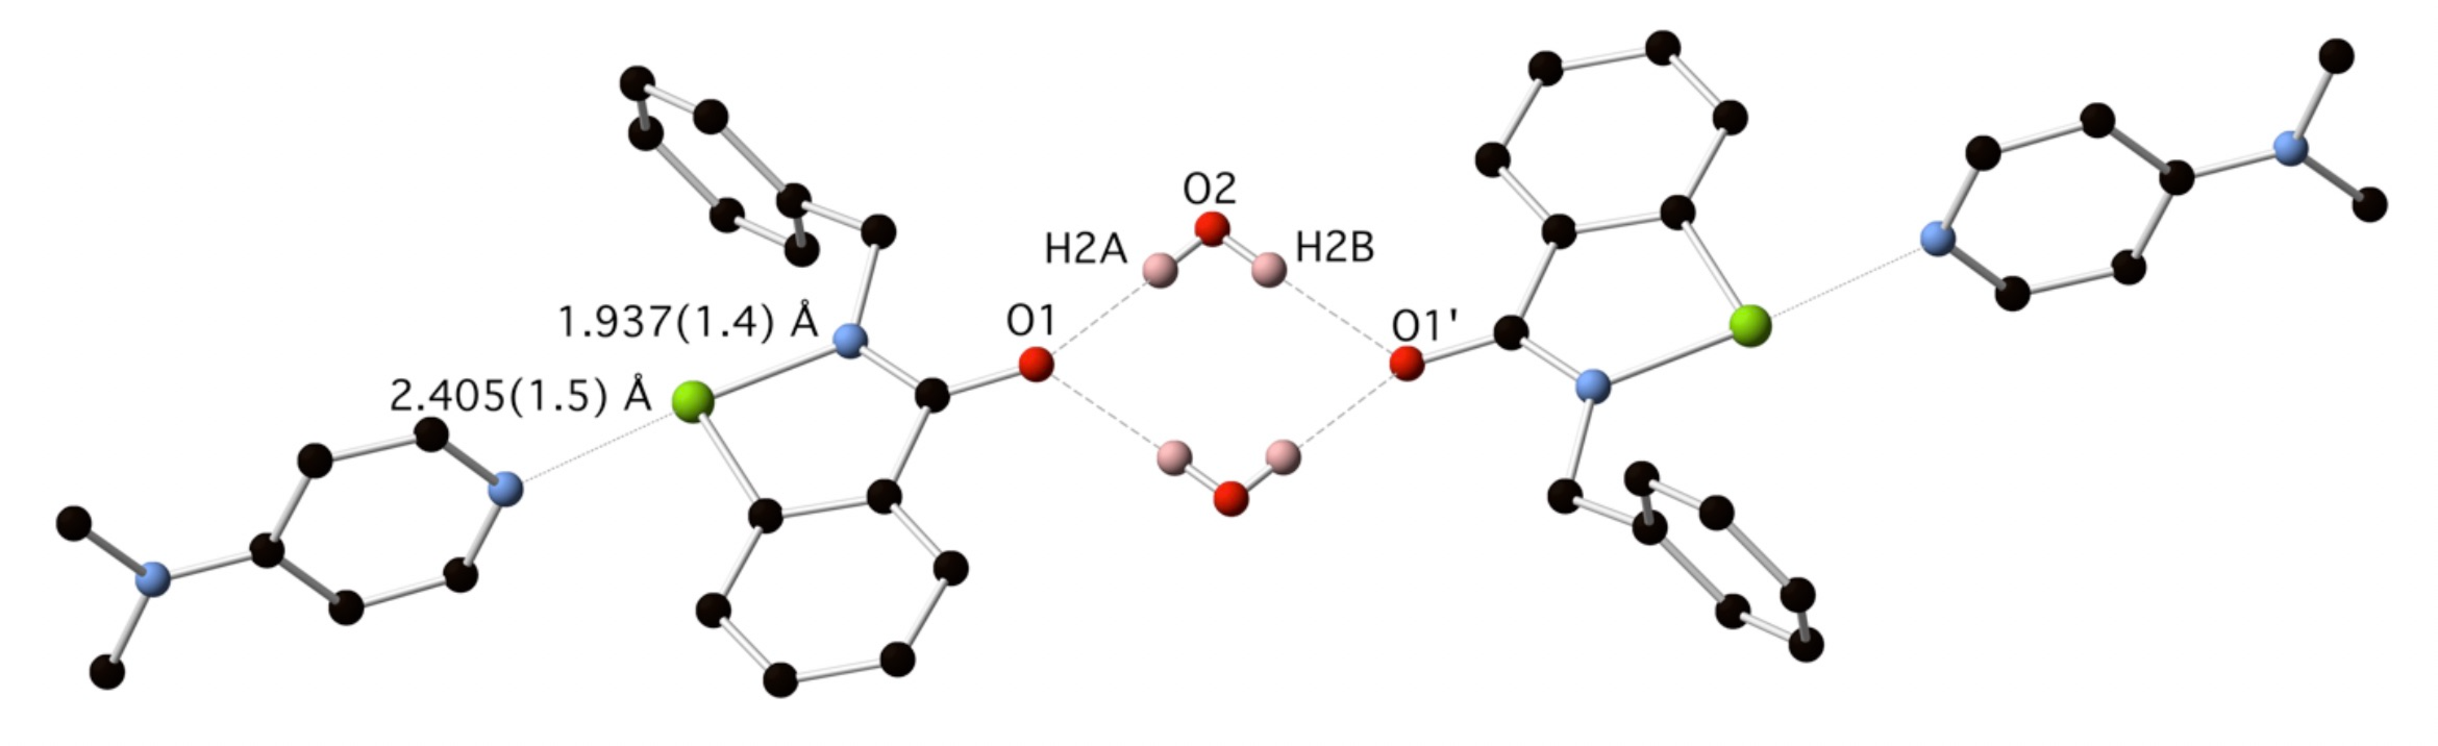
\includegraphics[width=0.8\linewidth]{Figures/benzyl-dmap-hydrate.pdf}
  \caption{Structure of \refcmpd{ebs.bn}$\cdot$DMAP$\cdot$\ce{H2O}.}
  \label{fig:benzyl-dmap-hydrate}
\end{figure}

\cmpd{ebs.bn}$\cdot$DMAP$\cdot$\ce{H2O} crystallizes as a centrosymmetric hydrogen-bonded dimer in which two water molecules bridge two molecules of \cmpd{ebs.bn} across a crystallographic inversion centre.
Of note, when comparison is made between the structural parameters for \cmpd{ebs.bn}$\cdot$DMAP molecule 1, which has a similar geometry about the N$\cdots$Se moiety as for \cmpd{ebs.bn}$\cdot$DMAP$\cdot$\ce{H2O}, there is a significant contraction of the N\textsubscript{DMAP}$\cdots$Se distance from 2.4276(14)~\AA\ to 2.4046(14)~\AA\ ($\Delta$=-0.023~\AA ; 16$\sigma$), and an increase in the Se--N\textsubscript{1} bond distance from 1.9297(13) to 1.9367(14)~\AA\ ($\Delta$=0.007~\AA ; 5$\sigma$).
We have coined the term `hydrogen-bond enhanced Ch-bonding' to describe this interesting structural effect.

\subsection{Effects of the Lewis base on Ch-bond strength}
We were fortunate to obtain crystal structures of the Se-tetracycle \cmpd{tetracycle} with both pyridine and DMAP, which gave us the opportunity to compare the structural effects arising from two Ch-bond acceptors with significantly different basicities.
The pyridine adduct of \cmpd{tetracycle} is characterized by a N\textsubscript{PYR}$\cdots$Se distance 2.461(3)~\AA\ and Se--N\textsubscript{1} distance of 1.926(2)~\AA\ and a near linear N\textsubscript{PYR}$\cdots$Se--N\textsubscript{1} angle, the Se--N\textsubscript{1} bond distance is significantly longer than the corresponding distance 1.883(2)~\AA\ in non-bound structure of \cmpd{tetracycle}.
The DMAP adduct of \cmpd{tetracycle} is characterized by a significantly shorter N\textsubscript{DMAP}$\cdots$Se distance of 2.304(1)~\AA\ ($\Delta$=-0.157~\AA) and longer Se--N\textsubscript{1} distance of 1.9716(9)~\AA\ ($\Delta$=0.046~\AA), consistent with a significantly stronger interaction.

\begin{figure}
  \centering
  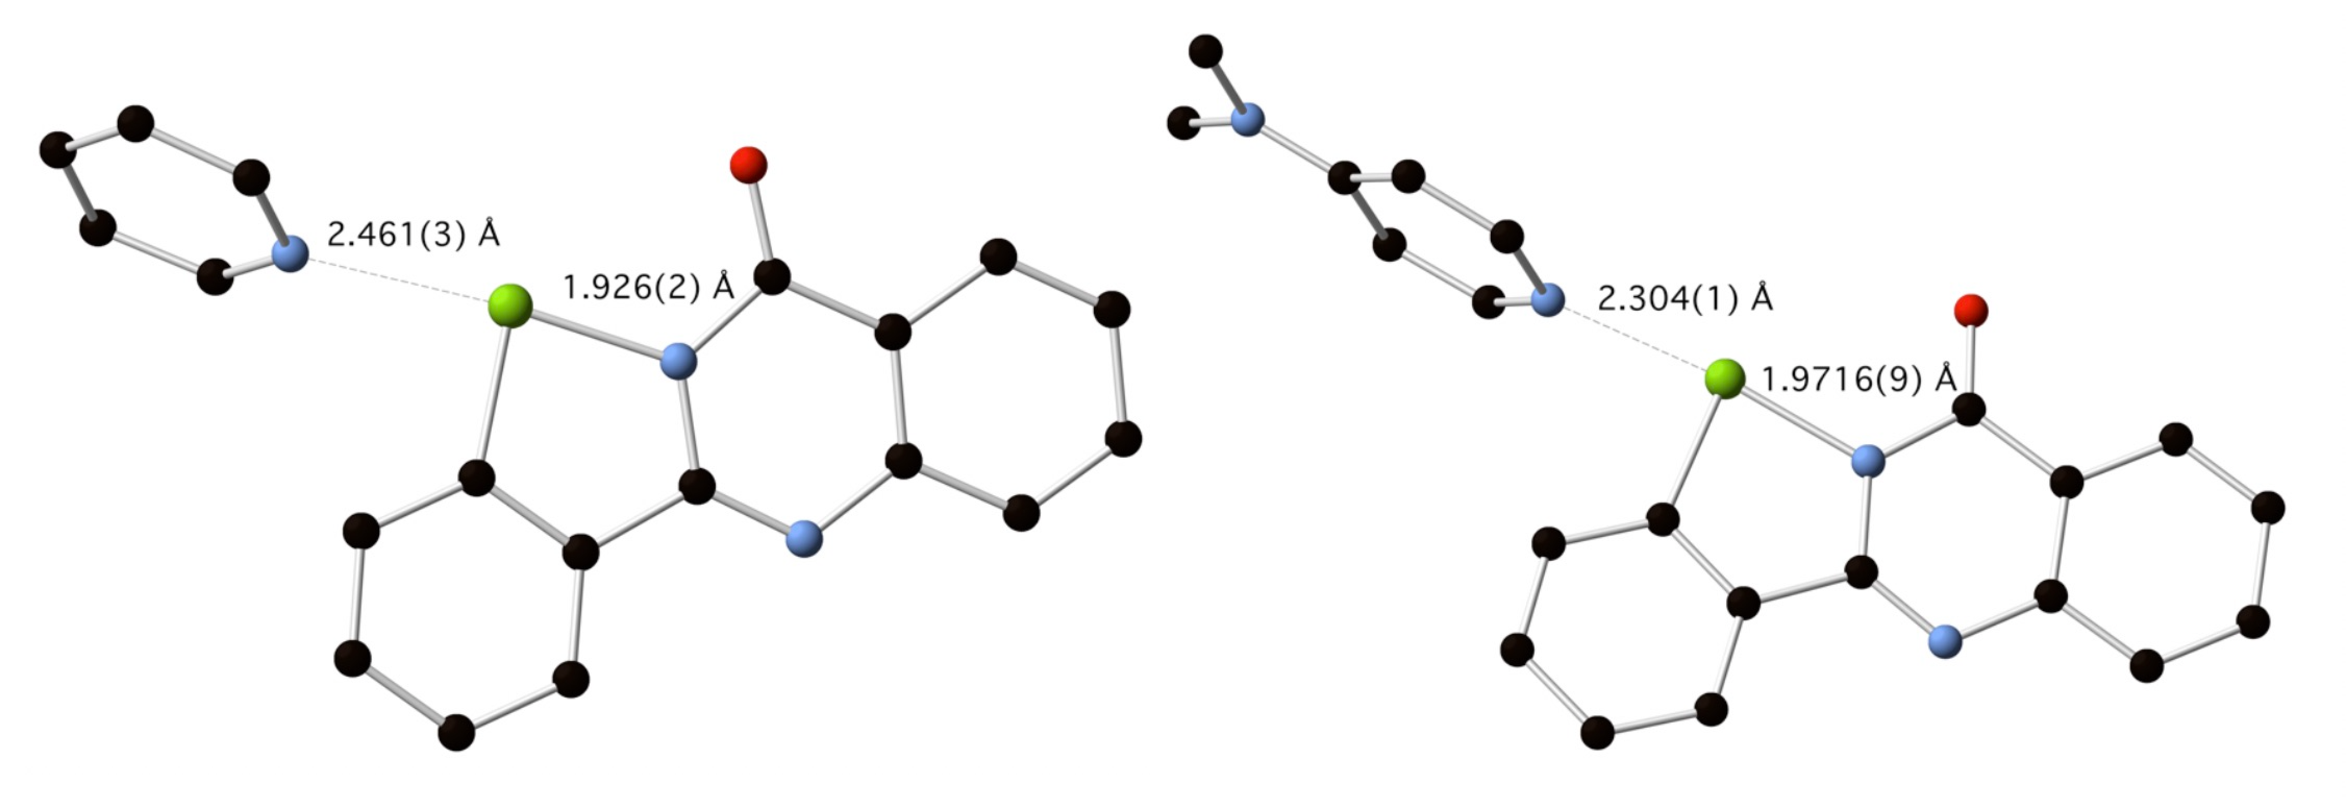
\includegraphics[width=0.8\linewidth]{Figures/dimer-dmap-py-xray.pdf}
  \caption{Pyridine and DMAP adducts of Se-tetracycle \refcmpd{tetracycle}.}
  \label{fig:dimer-adducts}
\end{figure}

Ch-bonded co-crystals of the benzisoselenazolinone derivative \cmpd{ebs.bn} with the tertiary amines; quinuclidine and DABCO were obtained and structurally characterized.
The adducts are presented in \cref{fig:benzyl-adducts}.
The N\textsubscript{QUIN}$\cdots$Se and N\textsubscript{DABCO}$\cdots$Se distances of 2.5874(17)~\AA\ and 2.6166(15)~\AA\ for \cmpd{ebs.bn}$\cdot$quinuclidine and \cmpd{ebs.bn}$\cdot$DABCO respectively are significantly longer than those observed for \cmpd{ebs.bn}$\cdot$DMAP suggesting an order of Ch-bond strengths with \cmpd{ebs.bn} DABCO < Quinuclidine < DMAP which correlates well with the hydrogen bond acceptor ability of these bases, as quantified by the pK\textsubscript{HB} (\cref{tab:pkhb}).

\begin{table}
  \centering
  \caption{Hydrogen bond basicities of bases studied.}
  \begin{tabular}{lllll}
    \toprule
                            & pyridine                      & DABCO                     & quinuclidine              & DMAP \\\midrule
      pK\textsubscript{HB}  & 1.86\autocite{Berthelot1998}  & 2.63\autocite{Graton2002} & 2.71\autocite{Graton2002} & 2.80\autocite{Berthelot1998}\\
      \cmpd{ebs.bn}$\cdot$base r(N$\cdots$Se) / \AA & ---   & 2.6166(15)                & 2.5874(17)                & 2.4276(14)\footnote{Bond distance given is the shorter of the two coordination environments.}\\
      \cmpd{ebs.bn}$\cdot$base $\Delta$H\textsubscript{f} / kcal/mol & -6.35    & -7.82 & ---                       & -7.91\\\bottomrule
  \end{tabular}
  \label{tab:pkhb}
\end{table}

\begin{figure}
  \centering
  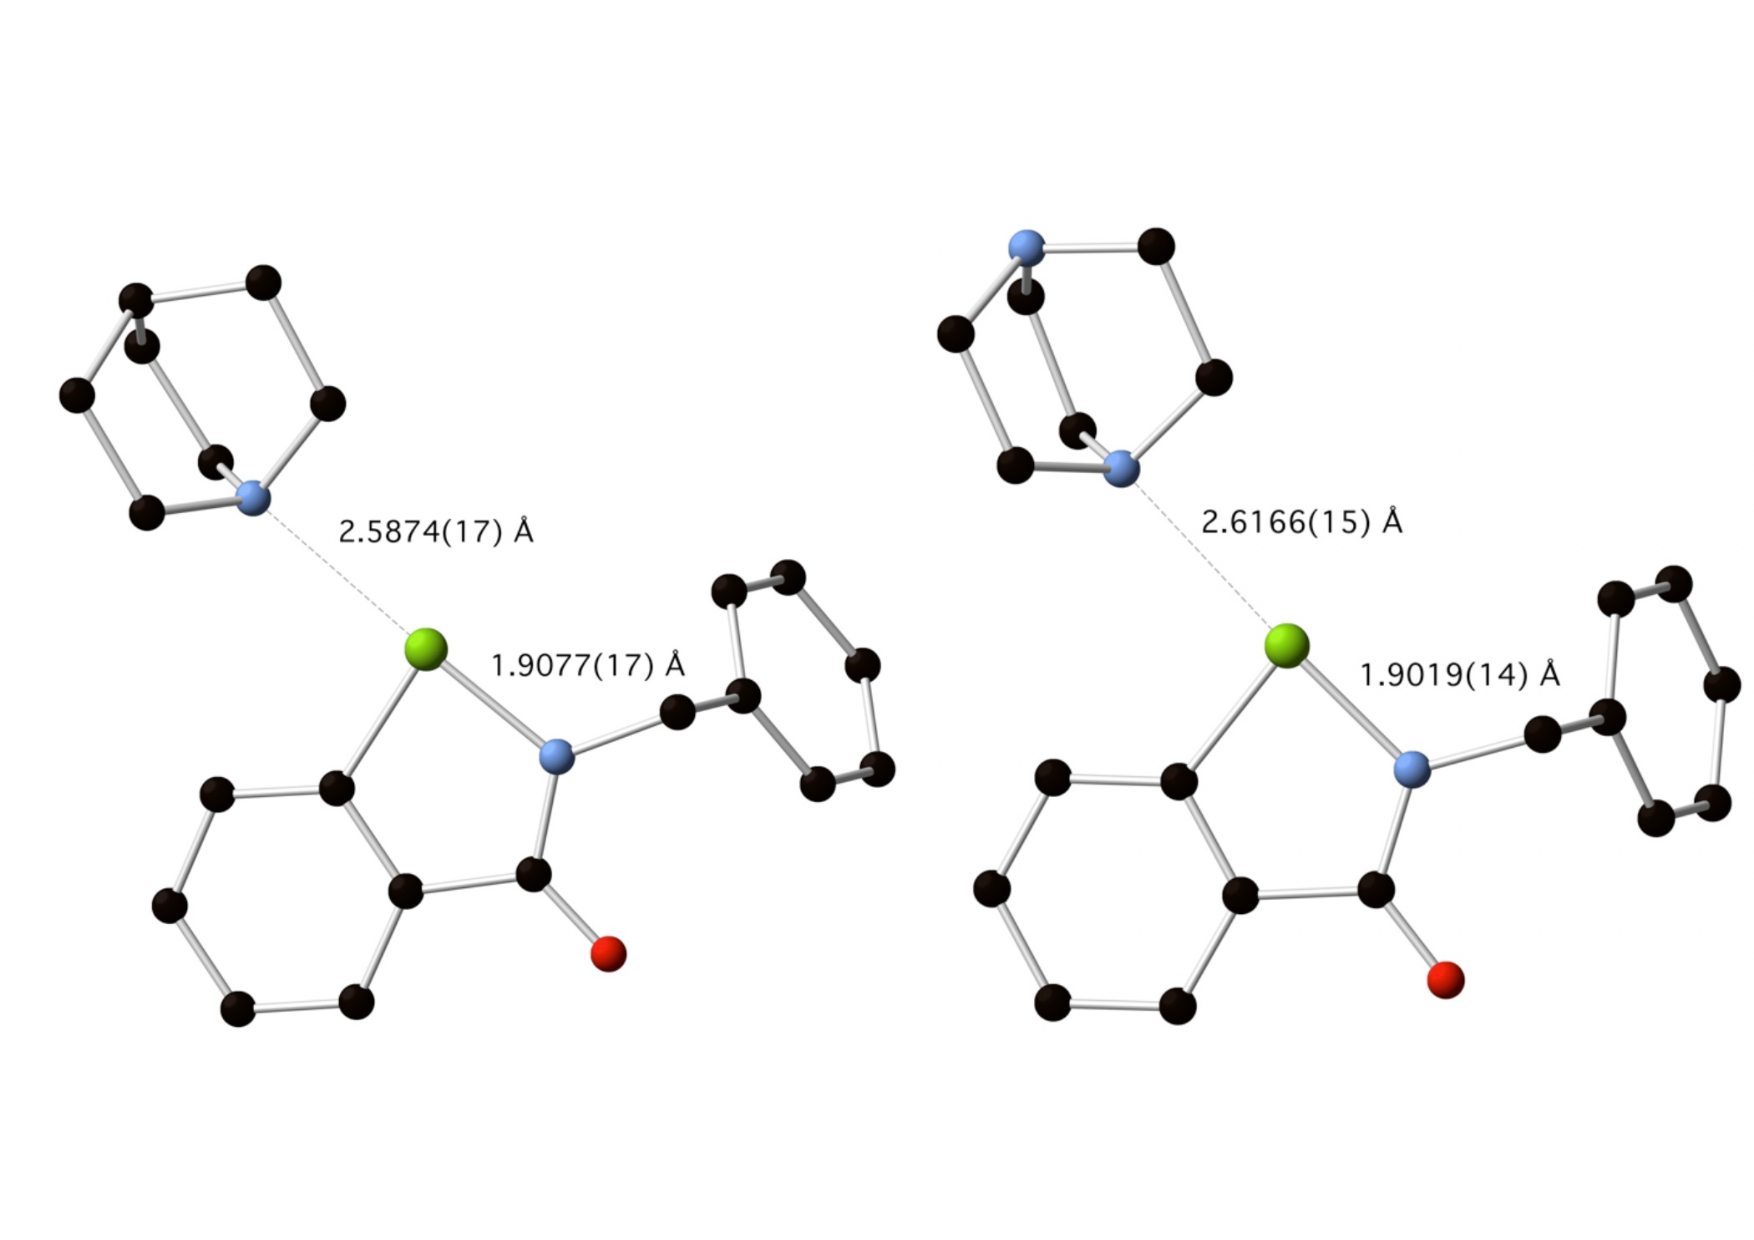
\includegraphics[width=0.8\linewidth]{Figures/benzyl-quin-dabco-xray.pdf}
  \caption{Adducts of benzisoselenazolinone \refcmpd{ebs.bn} with quinuclidine and DABCO.}
  \label{fig:benzyl-adducts}
\end{figure}

\subsection{DFT interaction energies, NBO and NEDA analysis}
Interaction energies for the complexes were calculated using the $\omega$B97X-D dispersion corrected functional, which has been used to study similar systems with good agreement with coupled cluster methods.\autocite{Oliveira2017}
All geometries were therefore optimized at $\omega$B97X-D/def2TZVP, and minima verified by frequency analysis.

\begin{figure}
  \centering
  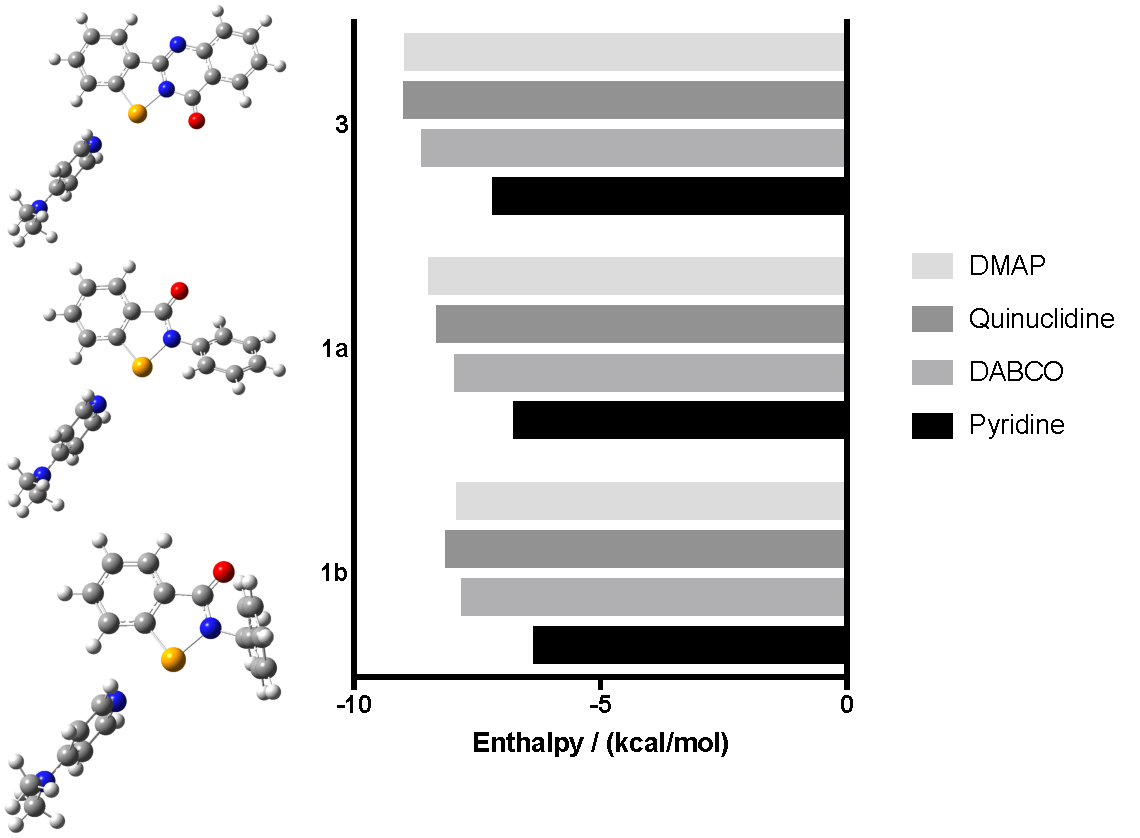
\includegraphics[width=0.8\linewidth]{Figures/dft-energies.pdf}
  \caption[Interaction energies for various complexes.]{Interaction enthalpies calculated at $\omega$B97X-D/def2TZVP. Optimised geometries for the DMAP complexes are shown to the left.}
\end{figure}

NBO analysis was conducted on the optimized geometries, which supports our suggestion that there is a strong orbital component to Ch-bonding in these systems.
Second order perturbation theory revealed that the energy associated with n(N\textsubscript{base})$\rightarrow$ $\sigma^{\star}$(N\textsubscript{1}--Se) delocalization was 12.79, 15.45, and 16.23~kcal/mol for \cmpd{ebs.bn}$\cdot$DMAP, \cmpd{ebs}$\cdot$DMAP, and \cmpd{tetracycle}$\cdot$DMAP respectively.
%In the case of the \cmpd{ebs.bn}$\cdot$DMAP$\cdot$\ce{H2O} complex, the delocalization energy was 13.51~kcal/mol.
%This consistent with our experimental observation of hydrogen-bond enhanced Ch-bonding.

\begin{figure}
  \centering
  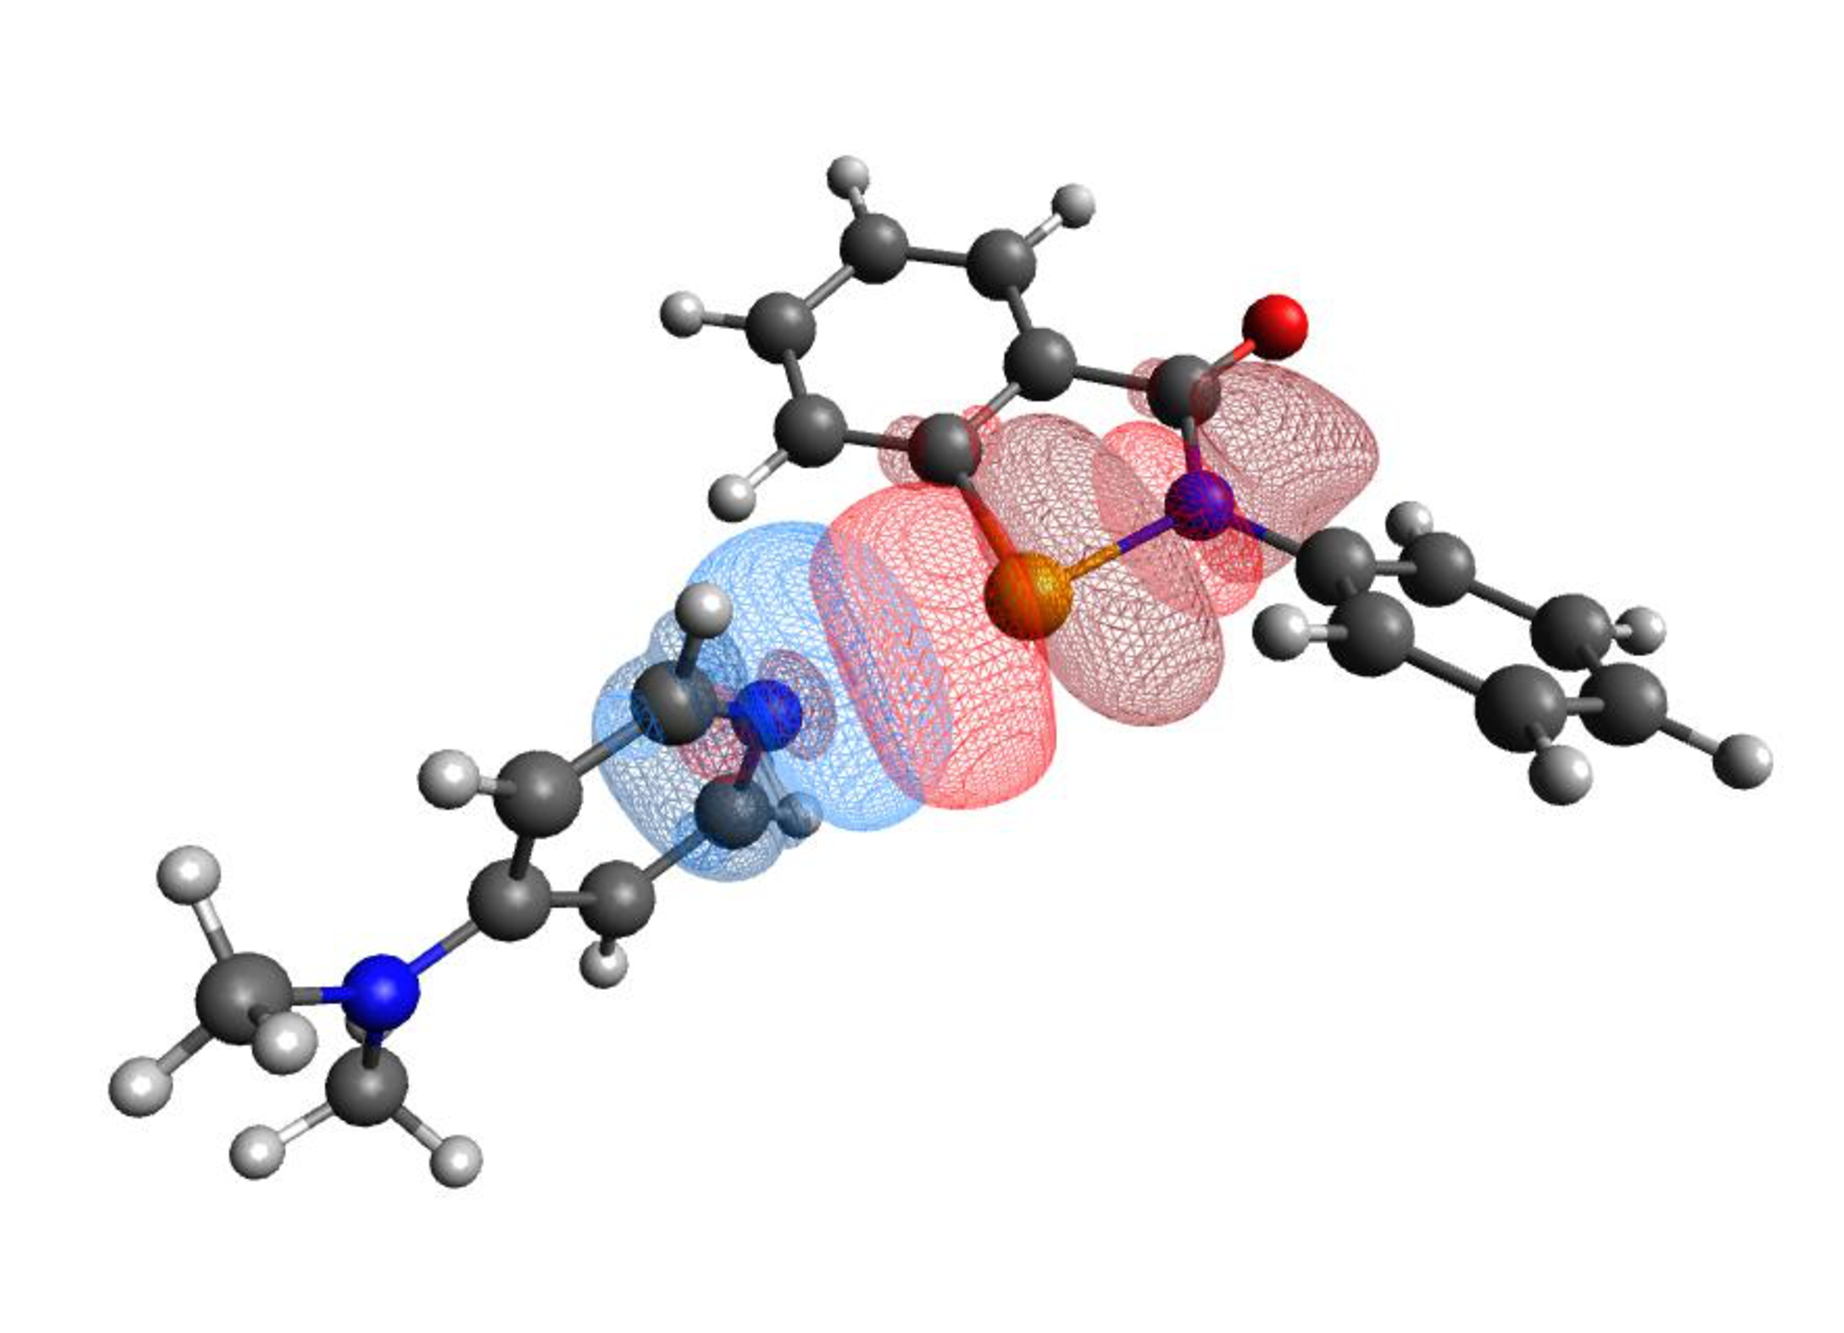
\includegraphics[width=0.6\linewidth]{Figures/phenyl-dmap-overlap.pdf}
  \caption[Orbital overlap for \refcmpd{ebs}$\cdot$DMAP.]{Overlap of nitrogen lone pair with $\sigma^{\star}$(Se - N) in \refcmpd{ebs}$\cdot$DMAP complex.}
  \label{fig:phenyl-dmap-overlap}
\end{figure}

\section{Conclusion}
In summary, we have demonstrated the importance of Ch-bonding between derivatives of ebselen \cmpd{ebs} and a variety of nitrogen bases.
These selenium-containing heterocycles form close contacts with electron pair donors, well within the Van der Waals radii, with predictable geometries consistent with the Ch-bonding model.
These interactions appear to be primarily due to orbital overlap as opposed to electrostatic or dispersion mediated effects, as evidenced by lengthening of the antipodal Se--N bond, and computational analysis, which is consistent with findings in related systems by Cockroft et al.\autocite{Pascoe2017}
We have also found that the strength of a Ch-bond can be enhanced via a hydrogen bond to the carbonyl group of the heterocycle.
We hope to exploit the strength and directionality of Ch-bonds in ebselen to target biomolecules such as nucleic acids and proteins using compounds containing the isoselenazolone moiety.

\section{Supplementary materials}

\subsection{Synthetic procedures}

\subsubsection[Preparation of \refcmpd{ebs}.]{Preparation of 2-phenylbenzo[\emph{d}][1,2]selenazol-3(2\emph{H})-one \refcmpd{ebs}.}

Copper iodide (98.4~mg, 0.517~mmol) and 1,10-phenanthroline (83.1~mg, 0.461~mmol) were stirred in anhydrous DMF (3~mL) for 15 mins at r.t., then 2-iodo-N-phenylbenz\-amide (653.2~mg, 2.021~mmol), selenium (196.9~mg, 2.495~mmol) and potassium carbonate (627.3~mg, 4.539~mmol) were added sequentially under a flow of argon.
The mixture was heated at 110\degree C for 8~h, when TLC showed consumption of starting material.
The mixture was then tipped into brine (30~mL) and stirred to form a brown precipitate, which was extracted into DCM (40~mL) and washed with water (2 $\times$ 20~mL).
The DCM solution was filtered through a silica plug, then evaporated, and the residue applied to a SNAP 25~g silica cartridge, eluting with a petroleum ether/ethyl acetate gradient.
The major peak was evaporated to afford colourless crystals of \cmpd{ebs} (378.8~mg, 69\%, m.p. 179.1--180.3\degree C, lit. mp 180--181\degree C). \textsuperscript{77}Se NMR $\delta$ 959.66.

\subsubsection[Preparation of \refcmpd{ebs.bn}.]{Preparation of 2-benzylbenzo[\emph{d}][1,2]selenazol-3(2\emph{H})-one \refcmpd{ebs.bn}.}

Copper iodide (95.8~mg, 0.503~mmol) and 1,10-phenanthroline (93.8~mg, 0.521~mmol) were stirred in anhydrous DMF (3~mL) for 15 mins at r.t., then N-benzyl-2-iodobenz\-amide (860.9~mg, 2.553~mmol), selenium (256.6~mg, 3.249~mmol) and potassium carbonate (542.2~mg, 3.923~mmol) were added sequentially under a flow of argon.
The mixture was heated at 110\degree C for 5~h, when TLC showed consumption of starting material.
The mixture was then tipped into brine (30~mL) and stirred to form a solid mass, which was dissolved in DCM (40~mL) and washed with water (2 $\times$ 20~mL).
The DCM solution was filtered through a silica plug, then evaporated, and the residue applied to a SNAP 50~g silica cartridge, eluting with a petroleum ether/ethyl acetate gradient.
The major peak was evaporated to afford pale yellow crystals of \cmpd{ebs.bn} (396.4~mg, 53\%, m.p. 137.8--138.8\degree C). \textsuperscript{77}Se NMR $\delta$ 884.02.

\subsubsection[Preparation of \refcmpd{tetracycle}.]{Preparation of 5\emph{H}-benzo[4,5][1,2]selenazolo[2,3-\emph{a}]quinazolin-5-one \refcmpd{tetracycle}.}

Copper iodide (96.4~mg, 0.503~mmol) and 1,10-phenanthroline (85.7~mg, 0.476~mmol) were stirred in anhydrous DMF (4~mL) for 10~mins at r.t., then 2-iodobenzamide (510.6~mg, 2.067~mmol), selenium (209.5~mg, 2.653~mmol) and potassium carbonate (506.3~mg, 3.663~mmol) were added sequentially under a flow of argon.
The mixture was heated at 110\degree C for 12~h, when TLC showed consumption of starting material.
The mixture was then tipped into brine (30~mL) and stirred to form a solid mass, which was extracted into ethyl acetate (20~mL) and washed with water (2 $\times$ 20~mL).
The DCM solution was filtered through a silica plug, then evaporated, and the residue applied to a SNAP 50~g silica cartridge, eluting with a petroleum ether/ethyl acetate gradient.
The major peak was evaporated to afford pale yellow crystals of \cmpd{tetracycle} (45.8~mg, 15\%, m.p. 267--268\degree C). \textsuperscript{77}Se NMR $\delta$ 992.48.

\subsection{Crystallographic data}
\label{sec:ch3-si}
Intensity data was collected on an Oxford Diffraction SuperNova CCD diffractometer using either Cu-K$\alpha$ or Mo-K$\alpha$ radiation at 130.0(1)~K, or on a Rigaku XtalLAB Synergy at 100.0(1)~K. Compound \cmpd{ebs.bn}$\cdot$DMAP$\cdot$\ce{H2O} underwent a destructive phase change when cooling to 130~K, therefore data were collected at 200~K. Data for \cmpd{tetracycle} was collected on the MX1 beamline at the Australian Synchrotron\autocite{Cowieson2015}. The temperature was maintained using an Oxford Cryostream cooling device. The structures were solved by direct methods and difference Fourier synthesis.\autocite{Sheldrick2015} Thermal ellipsoid plot was generated using the program ORTEP-3\autocite{Farrugia1997} integrated within the WINGX\autocite{Farrugia1999} suite of programs.

\subsubsection{Crystal data for \texorpdfstring{\refcmpd{ebs}$\cdot$DMAP}{C20H19N3OSe}}
\ce{C20H19N3OSe}, $M=396.34$, $T=130.0$~K, $\lambda=0.71073$~\AA, Triclinic, space group P$\bar{1}$, $a = 8.3674(3)$, $b = 9.8399(5)$, $c =10.6622(5)$~\AA, $\alpha=93.296(4)$\degree, $\beta=93.021(4)$\degree, $\gamma=101.210(4)$\degree, $V=857.86(7)$~\AA$^{3}$, $Z = 2$.
$D_{c}= 1.534$~mg~M$^{-3}$, $\mu$(Mo-K$\alpha$) = 2.201~mm$^{-1}$, F(000) = 404, crystal size $0.52 \times 0.34 \times 0.23$~mm.
11339 reflections measured, $\theta_{\mathrm{max}}=36.66$\degree, 7889 independent reflections, R\textsubscript{int} = 0.0163, the final R was 0.0293 ($I > 2\theta(I)$, 6882 reflections) and \emph{w}R(F\textsuperscript{2}) was 0.0721 (all data), GOF 0.992.
CCDC 1867205.
From dichloromethane/pentane (70\%) m.p. 111.3--112.1\degree C.

\begin{figure}
  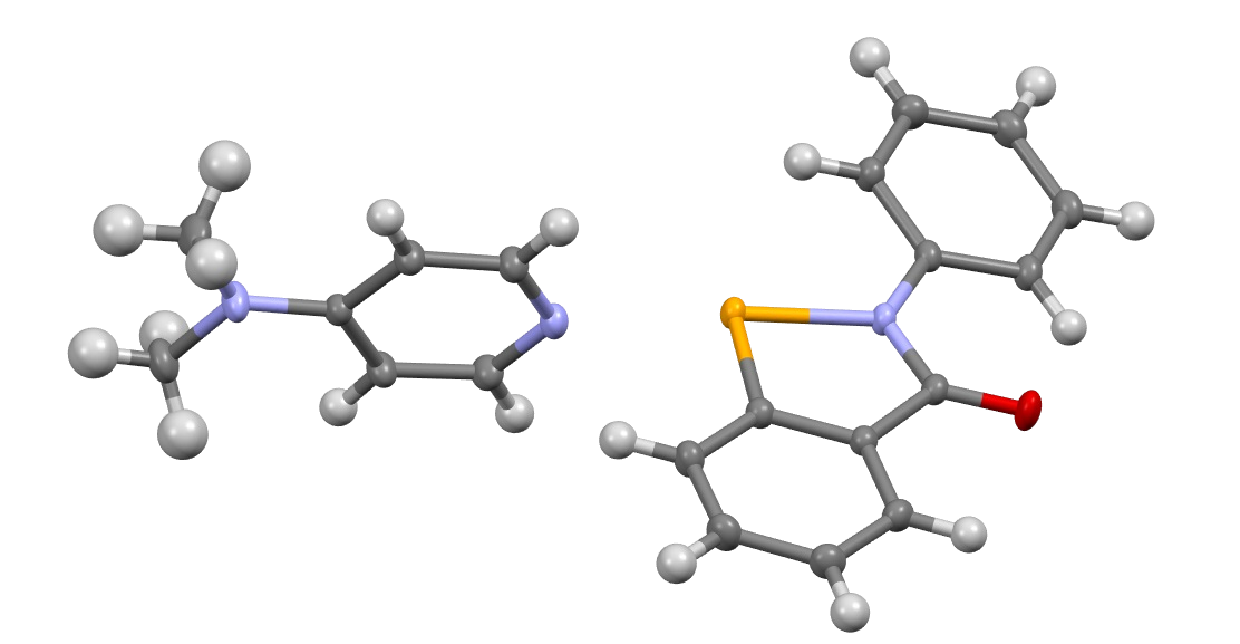
\includegraphics[width=0.6\linewidth]{Figures/ebs-dmap-xtal.pdf}
  \caption{X-ray crystal structure of \texorpdfstring{\refcmpd{ebs}$\cdot$DMAP}{C20H19N3OSe}.}
\end{figure}

\subsubsection{Crystal data for \texorpdfstring{\refcmpd{ebs.bn}}{C14H11NOSe}}
\ce{C14H11NOSe}, $M=288.20$, $T=100.0$~K, $\lambda=0.71073$~\AA, Orthorhombic, space group Pca2\textsubscript{1}, $a = 11.7848(3)$, $b = 4.5869(1)$, $c = 21.3572(5)$~\AA, $V = 1154.48(5)$~\AA$^{3}$, $Z = 4$.
$D_{c}= 1.658$~mg~M$^{-3}$, $\mu$(Mo-K$\alpha$) = 3.233~mm$^{-1}$, F(000) = 576, crystal size $0.63 \times 0.54 \times 0.22$~mm.
44918 reflections measured, $\theta_{\mathrm{max}}=45.38$\degree, 9588 independent reflections, R\textsubscript{int} = 0.0481, the final R was 0.0331 ($I > 2\theta(I)$, 7848 reflections) and \emph{w}R(F\textsuperscript{2}) was 0.0792 (all data), GOF 1.063.
CCDC 1867211.

\begin{figure}
  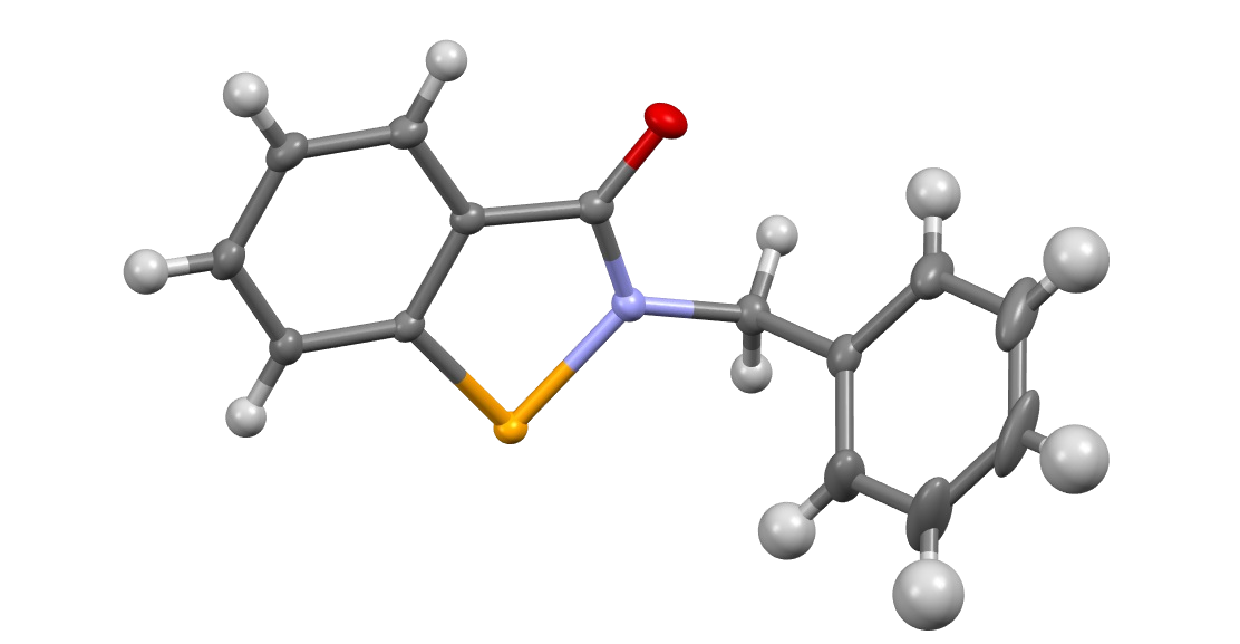
\includegraphics[width=0.6\linewidth]{Figures/ebs-bn-xtal.pdf}
  \caption{X-ray crystal structure of \texorpdfstring{\refcmpd{ebs.bn}}{C14H11NOSe}.}
\end{figure}

\subsubsection{Crystal data for \texorpdfstring{\refcmpd{ebs.bn}$\cdot$DMAP$\cdot$\ce{H2O}}{C21H21N3OSe.(H2O)}}
\ce{C21H21N3OSe.(H2O)}, $M=428.38$, $T=200.0$~K, $\lambda=0.71073$~\AA, Triclinic, space group P$\bar{1}$, $a = 9.6254(2)$, $b = 10.2486(2)$, $c = 10.6505(2)$~\AA, $\alpha = 83.660(2)$\degree, $\beta = 76.398(2)$\degree, $\gamma = 78.423(2)$\degree, $V = 998.19(4)$~\AA$^{3}$, $Z = 2$.
$D_{c}= 125$~mg~M$^{-3}$, $\mu$(Mo-K$\alpha$) = 1.901~mm$^{-1}$, F(000) = 440, crystal size $0.41 \times 0.32 \times 0.23$~mm.
30047 reflections measured, $\theta_{\mathrm{max}} = 41.06$\degree, 12528 independent reflections, R\textsubscript{int} = 0.0267, the final R was 0.0456 ($I > 2\theta(I)$, 6303 reflections) and \emph{w}R(F\textsuperscript{2}) was 0.1219 (all data), GOF 1.000.
CCDC 1867213.
From THF in an open flask (90\%) m.p. 96--97\degree C.

\begin{figure}
  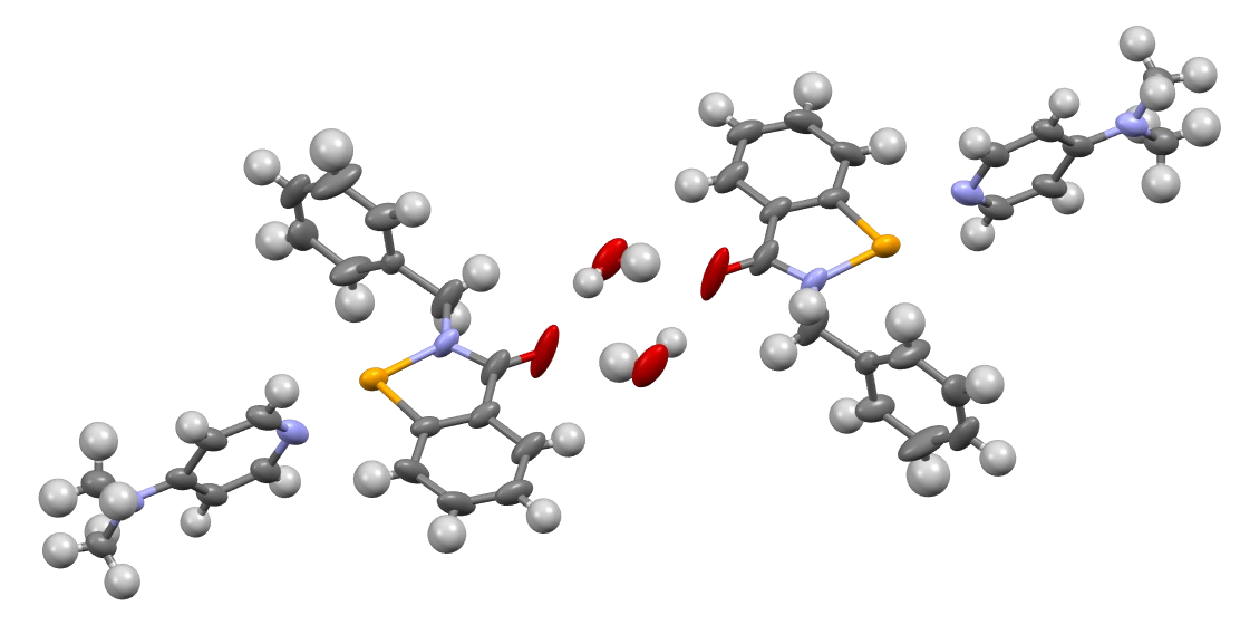
\includegraphics[width=0.6\linewidth]{Figures/ebs-bn-dmap-hydrate-xtal.pdf}
  \caption{X-ray crystal structure of \texorpdfstring{\refcmpd{ebs.bn}$\cdot$DMAP$\cdot$\ce{H2O}}{C21H21N3OSe.(H2O)}.}
\end{figure}

\subsubsection{Crystal data for \texorpdfstring{\refcmpd{ebs.bn}$\cdot$DMAP}{C21H21N3OSe}}
\ce{C21H21N3OSe}, $M=410.37$, $T=130.0$~K, $\lambda=0.71073$~\AA, Triclinic, space group P$\bar{1}$, $a = 9.6002(4)$, $b = 10.2109(4)$, $c = 19.8380(7)$~\AA, $\alpha = 78.710(3)$\degree, $\beta = 84.901(3)$\degree, $\gamma = 77.458(4)$\degree, $V = 1859.33(13)$~\AA$^{3}$, $Z = 4$, $Z\prime = 2$.
$D_{c}= 1.466$~mg~M$^{-3}$, $\mu$(Mo-K$\alpha$) = 2.034~mm$^{-1}$, F(000) = 840, crystal size $0.65 \times 0.24 \times 0.37$~mm.
36541 reflections measured, $\theta_{\mathrm{max}} = 40.95$\degree, 23437 independent reflections, R\textsubscript{int} = 0.0264, the final R was 0.0448 ($I > 2\theta(I)$, 15177 reflections) and \emph{w}R(F\textsuperscript{2}) was 0.1120 (all data), GOF 1.044.
CCDC 1867209.
From dichloromethane/pentane (60\%) m.p. 86.1--92.5\degree C.

\begin{figure}
  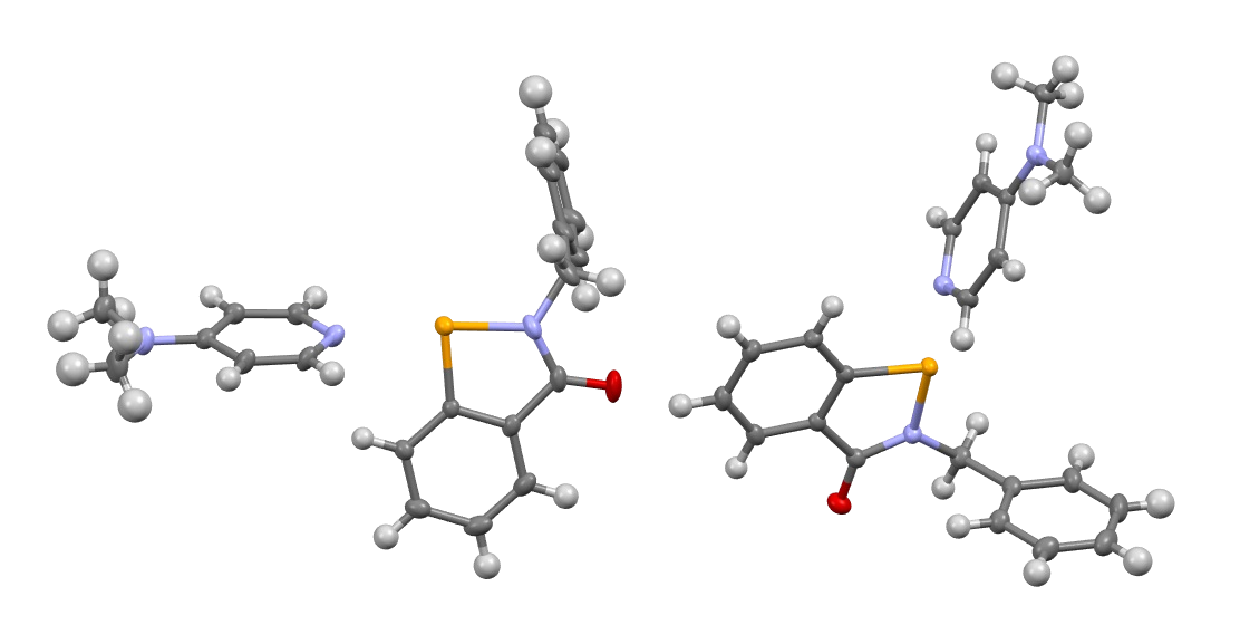
\includegraphics[width=0.6\linewidth]{Figures/ebs-bn-dmap-xtal.pdf}
  \caption{X-ray crystal structure of \texorpdfstring{\refcmpd{ebs.bn}$\cdot$DMAP}{C21H21N3OSe}.}
\end{figure}

\subsubsection{Crystal data for \texorpdfstring{\refcmpd{ebs.bn}$\cdot$quinuclidine}{C21H24N2OSe}}
\ce{C21H24N2OSe}, $M=399.38$, $T=130.0$~K, $\lambda=1.54184$~\AA, Monoclinic, space group P2\textsubscript{1}/c, $a = 10.1610(2)$, $b = 16.0506(3)$, $c = 11.4300(2)$~\AA, $\beta = 104.622(2)$\degree, $V = 1803.75(6)$ \AA$^{3}$, $Z = 4$.
$D_{c}= 1.471$~mg~M$^{-3}$, $\mu$(Cu-K$\alpha$) = 3.895~mm$^{-1}$, F(000) = 824, crystal size $0.29 \times 0.10 \times 0.03$~mm.
12588 reflections measured, $\theta_{\mathrm{max}} = 77.19$\degree, 3771 independent reflections, R\textsubscript{int} = 0.0379, the final R was 0.0329 ($I > 2\theta(I)$, 3397 reflections) and \emph{w}R(F\textsuperscript{2}) was 0.0849 (all data), GOF 1.028.
CCDC 1867207.
From dichloromethane/pentane (50\%) m.p. 135.2--137.4\degree C.

\begin{figure}
  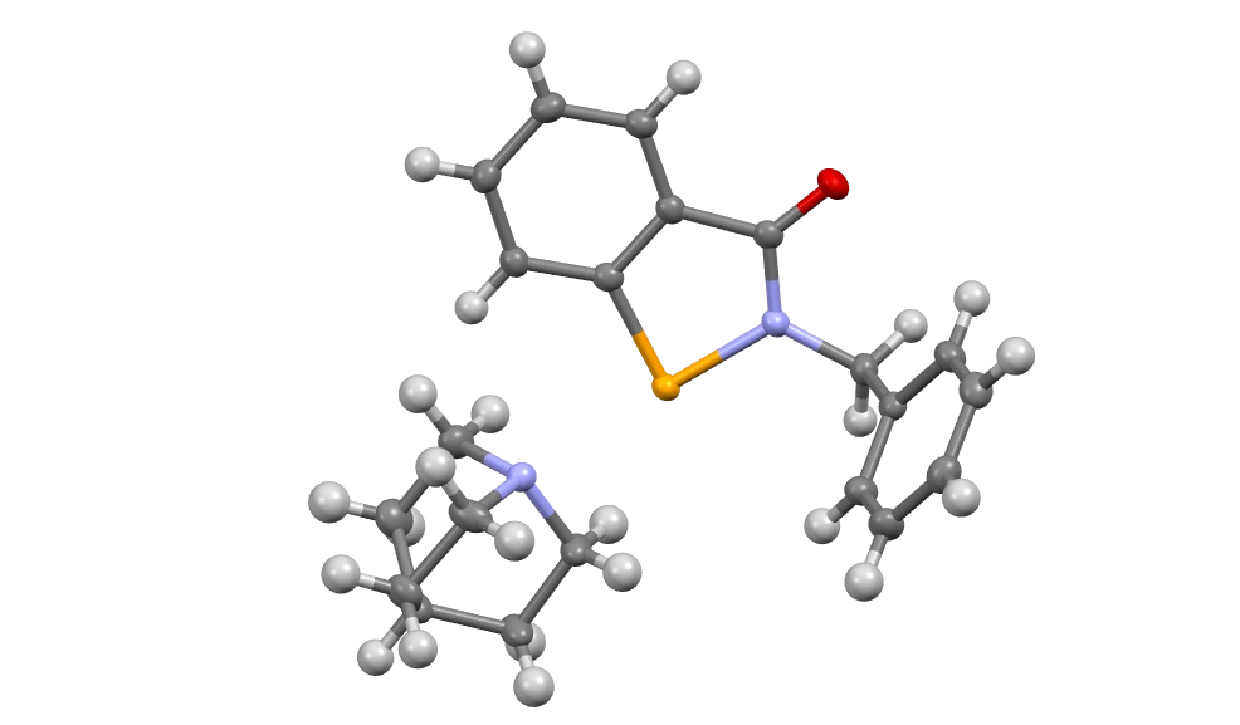
\includegraphics[width=0.6\linewidth]{Figures/ebs-bn-quin-xtal.pdf}
  \caption{X-ray crystal structure of \texorpdfstring{\refcmpd{ebs.bn}$\cdot$quinuclidine}{C21H24N2OSe}.}
\end{figure}

\subsubsection{Crystal data for \texorpdfstring{\refcmpd{ebs.bn}$\cdot$DABCO}{C20H23N3OSe}}
\ce{C20H23N3OSe}, $M=400.37$, $T=130.0$~K, $\lambda=1.54184$~\AA, Monoclinic, space group P2\textsubscript{1}/c, $a = 10.1249(2)$, $b = 15.9246(3)$, $c = 11.4660(2)$~\AA, $\beta = 106.572(2)$\degree, $V = 1771.93(6)$ \AA$^{3}$, $Z = 4$.
$D_{c} = 1.501$~mg~M$^{-3}$, $\mu$(Cu-K$\alpha$) = 2.965~mm$^{-1}$, F(000) = 824, crystal size $0.37 \times 0.17 \times 0.04$~mm.
13121 reflections measured, $\theta_{\mathrm{max}} = 77.12$\degree, 3711 independent reflections, R\textsubscript{int} = 0.0280, the final R was 0.0258 ($I > 2\theta(I)$, 3333 reflections) and \emph{w}R(F\textsuperscript{2}) was 0.0657 (all data), GOF 1.056.
CCDC 1867206.
From dichloromethane/pentane (65\%) m.p. 131.4--133.3\degree C.

\begin{figure}
  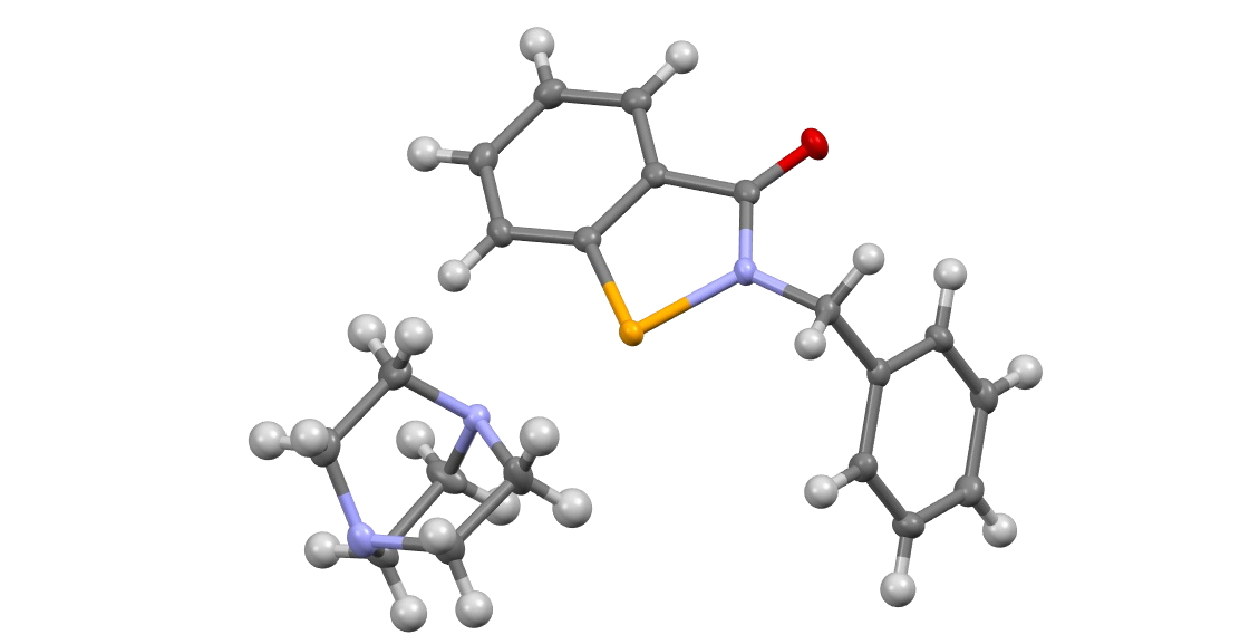
\includegraphics[width=0.6\linewidth]{Figures/ebs-bn-dabco-xtal.pdf}
  \caption{X-ray crystal structure of \texorpdfstring{\refcmpd{ebs.bn}$\cdot$DABCO}{C20H23N3OSe}.}
\end{figure}

\subsubsection{Crystal data for \texorpdfstring{\refcmpd{tetracycle}}{C14H8N2OSe}}
\ce{C14H8N2OSe}, $M=299.18$, $T=100.0$~K, $\lambda=0.71092$~\AA, Orthorhombic, space group Pca2\textsubscript{1}, $a = 17.371(4)$, $b = 5.3080(11)$, $c = 11.633(2)$~\AA, $V = 1072.6(4)$~\AA$^{3}$, $Z = 4$.
$D_{c}= 1.853$~mg~M$^{-3}$, $\mu$(Mo-K$\alpha$) = 3.486~mm$^{-1}$, F(000) = 592, crystal size $0.15 \times 0.10 \times 0.02$~mm.
16031 reflections measured, $\theta_{\mathrm{max}}=31.56$\degree, 2967 independent reflections, R\textsubscript{int} = 0.0363, the final R was 0.0271 ($I > 2\theta(I)$, 2061 reflections) and \emph{w}R(F\textsuperscript{2}) was 0.0751 (all data), GOF 1.129.
CCDC 1867208.

\begin{figure}
  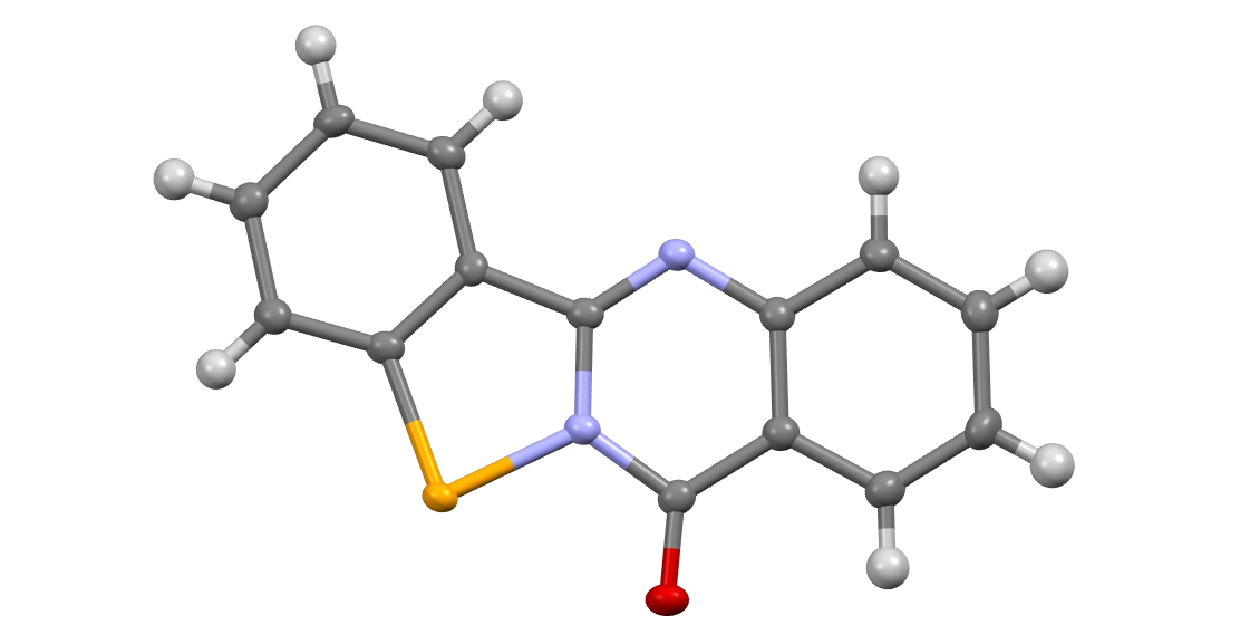
\includegraphics[width=0.6\linewidth]{Figures/tetracycle-xtal.pdf}
  \caption{X-ray crystal structure of \texorpdfstring{\refcmpd{tetracycle}}{C14H8N2OSe}.}
\end{figure}

\subsubsection{Crystal data for \texorpdfstring{\refcmpd{tetracycle}$\cdot$pyridine}{C19H13N3OSe}}
\ce{C19H13N3OSe}, $M=378.28$, $T=130.0$~K, $\lambda=1.54184$~\AA, Monoclinic, space group P2\textsubscript{1}/c, $a = 20.7476(9)$, $b = 4.9407(2)$, $c = 17.6687(7)$~\AA, $\beta = 107.376(4)$\degree, $V = 1156.27(5)$ \AA$^{3}$, $Z = 4$.
$D_{c} = 1.454$~mg~M$^{-3}$, $\mu$(Cu-K$\alpha$) = 3.018~mm$^{-1}$, F(000) = 760, crystal size $0.56 \times 0.05 \times 0.03$~mm.
5766 reflections measured, $\theta_{\mathrm{max}} = 75.76$\degree, 3419 independent reflections, R\textsubscript{int} = 0.0301, the final R was 0.0346 ($I > 2\theta(I)$, 2889 reflections) and \emph{w}R(F\textsuperscript{2}) was 0.0955 (all data), GOF 1.054.
CCDC 1867211.
From dichloromethane/pentane (70\%) m.p. 247.5--248.4\degree C.

\begin{figure}
  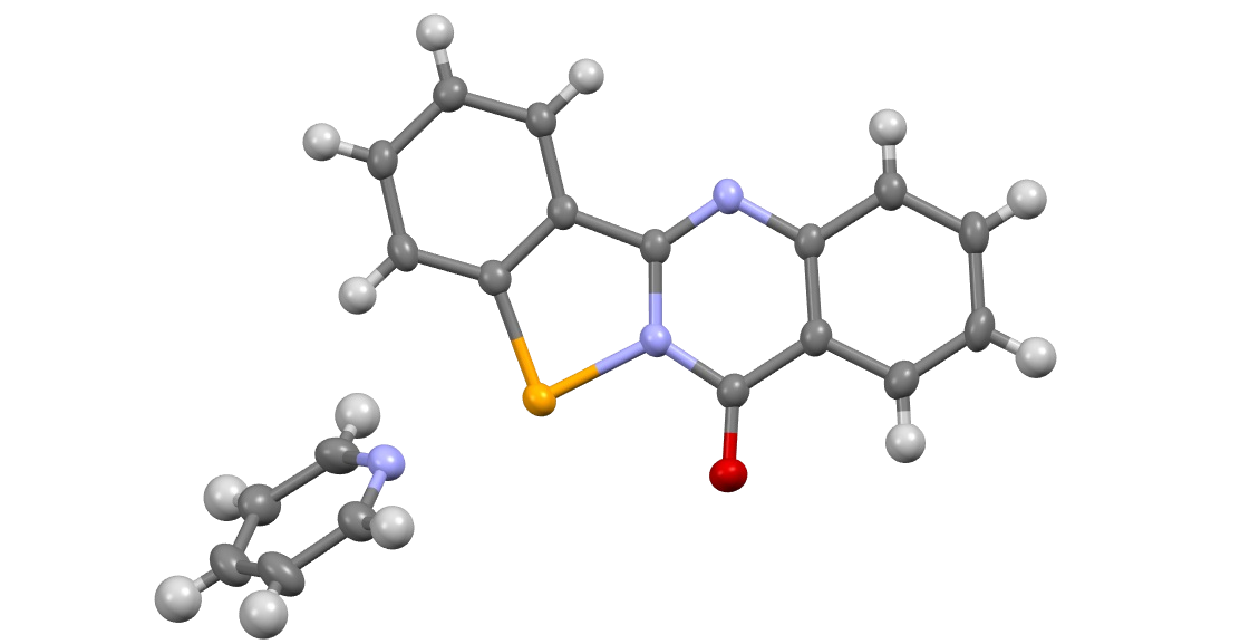
\includegraphics[width=0.6\linewidth]{Figures/tetracycle-py-xtal.pdf}
  \caption{X-ray crystal structure of \texorpdfstring{\refcmpd{tetracycle}$\cdot$pyridine}{C19H13N3OSe}.}
\end{figure}

\subsubsection{Crystal data for \texorpdfstring{\refcmpd{tetracycle}$\cdot$DMAP}{C21H18N4OSe}}
\ce{C21H18N4OSe}, $M = 421.35$, $T=100.0$~K, $\lambda=0.71073$~\AA, Triclinic, space group P$\bar{1}$, $a = 8.8093(2)$, $b = 10.7445(2)$, $c = 10.9812(2)$~\AA, $\alpha = 111.687(2)$\degree, $\beta = 109.283(2)$\degree, $\gamma = 96.631(2)$\degree, $V = 877.57(3)$~\AA$^{3}$, $Z = 2$, $Z\prime = 2$.
$D_{c}= 1.595$~mg~M$^{-3}$, $\mu$(Mo-K$\alpha$) = 2.159~mm$^{-1}$, F(000) = 428, crystal size $0.18 \times 0.11 \times 0.06$~mm.
56053 reflections measured, $\theta_{\mathrm{max}} = 41.07$\degree, 11273 independent reflections, R\textsubscript{int} = 0.0547, the final R was 0.0358 ($I > 2\theta(I)$, 8667 reflections) and \emph{w}R(F\textsuperscript{2}) was 0.0872 (all data), GOF 1.048.
CCDC 1867212.
From dichloromethane/pentane (80\%) m.p. 248.8--249.4\degree C.

\begin{figure}
  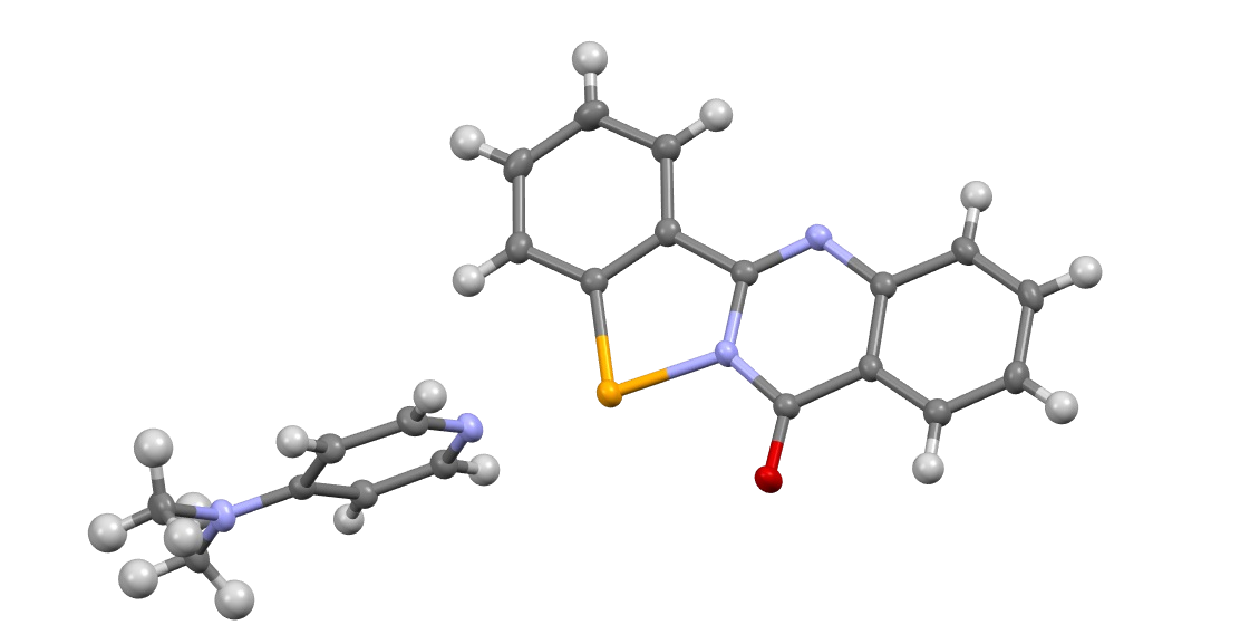
\includegraphics[width=0.6\linewidth]{Figures/tetracycle-dmap-xtal.pdf}
  \caption{X-ray crystal structure of \texorpdfstring{\refcmpd{tetracycle}$\cdot$DMAP}{C21H18N4OSe}.}
\end{figure}

\printbibliography[heading=subbibliography]
\end{refsection}


\begin{refsection}

\chapter{Further investigations into Ch-bonded complexes}

\section{Introduction}
In the previous chapter, we established that Ch-bonding is not only present in ebselen derivatives, but dominates packing in crystals of the pure compound (through \ce{Se\cdots O} interactions) and in co-crystals with a variety of Lewis bases.
In this chapter, we extend our investigation to a wider range of derivatives with systematically varied electronic properties.

Linear free energy relationships (LFERs) relate the rate of a chemical reaction with some electronic property of the substrate molecule(s).
Although the single crystal structures presented here are \emph{static} snapshots of reality, we can think of them as representative of the transition state of the breaking of the endocyclic \ce{Se-N} bond (\cref{fig:bond-breaking}).
The lower the transition state energy, the shorter will be the \ce{Se\dots N} Ch-bond distance, and this is clearly influenced by the electronic properties of both the Ch-bond donor and acceptor.

\begin{figure}
  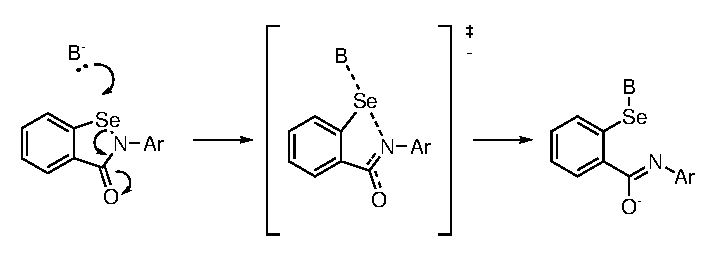
\includegraphics[scale=0.74]{Figures/bond-breaking.eps}
  \caption[Nucleophilic substitution at selenium.]{Depiction of the bond breaking/forming process of which Ch-bonding is a ground state manifestation.}
  \label{fig:bond-breaking}
\end{figure}

\section{Results and discussion}
Our previous work had shown that electron-rich pyridines (specifically DMAP) formed the strongest Ch-bonds out of all the bases trialled (\cref{sec:crystengcomm1}).
This is roughly consistent with the hydrogen bond basicity (pK\textsubscript{HB}) of the bases (\cref{tab:pkhb}).
The planar geometry and aromatic character of DMAP may also facilitate crystallisation, as opposed to the relatively bulky and flexible aliphatic bases which may not pack as efficiently.
For these reasons, we restricted the bases used in this study to other electron-rich pyridines.
Although DMAP is already a very strong base, the basisicity can be increased by incorporating the aniline nitrogen in another ring.
This reduces the energetic penalty associated with the delocalisation of the lone pair into the pyridine ring, by forcing a more planar geometry upon the nitrogen.\autocite{Berthelot1998,Heinrich2003EnhancingFixation}
Compounds \cmpd{py.pyrrol,py.morph} were therefore synthesised by treating 4-chloropyridine hydrochloride with 2 equivalents of the appropriate base (\cref{sch:base-synthesis}).

\begin{scheme}
\centering
\replacecmpd[sub-only]{py.pyrrol}
\replacecmpd[sub-only]{py.morph}
\replacecmpd{py.pyrrol,py.morph}
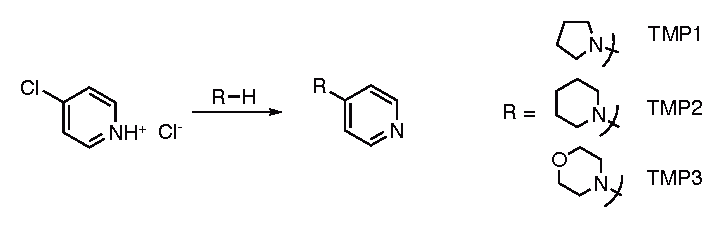
\includegraphics[scale=0.74]{Figures/base-synthesis.eps}
\caption{Synthesis of Lewis bases \refcmpd{py.pyrrol,py.morph}.}
\label{sch:base-synthesis}
\end{scheme}

The benzisoselenazolone derivatives \cmpd[merge=false,compress=false]{ebs,ebs.{4no2,4cn,4cf3,4br,4co2et,4me,4ome,4oet}} were prepared by the reaction of substituted anilines with a selenenyl chloride intermediate \cmpd{diselenide}, ultimately derived from anthranilic acid (\cref{sch:ebs-synthesis}).
The one-pot selenocyclisation reaction used in \cref{sec:crystengcomm1} often did not tolerate the various functional groups on the aryl ring, affording reduction, cross-coupling, or protodehalogenation byproducts.
All derivatives except \cmpd{ebs.4no2} were isolated in acceptable yield at room temperature using acetonitrile as a solvent, and in the presence of a weak base (triethylamine).
Due to the strongly electron-withdrawing nature of the nitro substituent, the parent aniline of \cmpd{ebs.4no2} was not sufficiently nucleophilic to react under the same conditions.
We therefore first deprotonated the aniline using \ce{NaH} (60\% suspension in mineral oil) in anhydrous THF before adding the selenyl chloride, which afforded the benzisoselenazolone in excellent yield.

We also note the solubility trends of the products as the electron demand of the substituent increases.
The electron rich derivatives \cmpd[merge=false,compress=false]{ebs.4ome,ebs.4oet,ebs.4me} were highly soluble even in relatively poor solvents (\ce{Et2O}, \ce{EtOAc}), while the electron poor derivatives \cmpd{ebs.4no2,ebs.4cn} were insoluble in all but the strongest solvents (DMSO).
This likely reflects the varying strength of the crystal packing due to the \ce{Se\cdots O=C} Ch-bond.

\begin{scheme}
\centering
\replacecmpd{diselenide}
\replacecmpd[merge=false,compress=false]{ebs}
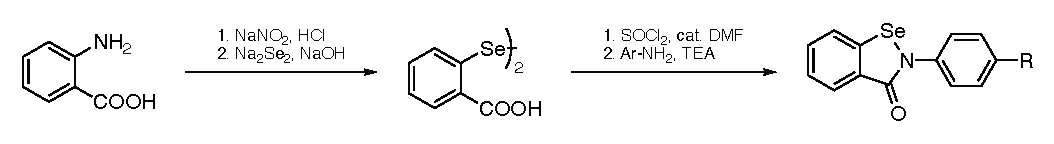
\includegraphics[scale=0.74]{Figures/ebs-synthesis.eps}

\begin{comment}
\vspace{0.6cm}

\footnotesize{
\begin{tabular}{cccccc}\toprule
    Compound & R = & Compound & R = & Compound & R = \\\midrule
    \cmpd{ebs} & \ce{-H} & \cmpd{ebs.4cf3} & \ce{-CF3} & \cmpd{ebs.4me} & \ce{-CH3}\\
    \cmpd{ebs.4no2} & \ce{-NO2} & \cmpd{ebs.4br} & \ce{-Br} & \cmpd{ebs.4ome} & \ce{-OMe}\\
    \cmpd{ebs.4cn} & \ce{-CN} & \cmpd{ebs.4co2et} & \ce{-CO2Et} & \cmpd{ebs.4oet} & \ce{-OEt} \\\bottomrule
\end{tabular}}
\end{comment}

\caption{Synthesis of benzisoselenazolone derivatives.}

\label{sch:ebs-synthesis}
\end{scheme}

Co-crystals of the benzisoselenazolones and pyridines were grown by vapour diffusion from an equimolar solution in dichloromethane/pentane.
Relevant structural parameters are given in \cref{tab:bondlengths2}.
In addition to the structural parameters, we characterised the various Ch-bonds using Bader's QTAIM framework.
Depending on the quality of the data we were able to obtain for each crystal, we used:

\begin{itemize}
    \item experimental electron density from a multipole refinement with atomic coordinates determined from high angle refinement ($d < 0.8$\AA),
    \item experimental electron density from a multipole refinement with atomic coordinates determined by refinement using aspherical scattering factors derived from the DFT electron density,
    \item density derived from a DFT calculation on the crystal geometry.
\end{itemize}

The second ``hybrid'' strategy has the advantage of being able to capture electron density effects not fully described by DFT, while not requiring a large amount of weak high-angle (or neutron) data for the reliable determination of atomic coordinates.
The low-angle data, however, does need to be free from faults, so this strategy may still not be appropriate for all data sets.

For the second and third strategies, the densities and scattering factors were calculated using NoSphereA2 incorporated in Olex2.\autocite{Kleemiss2021}

\begin{table}
  \centering
  \caption{Selected structural and electron density parameters of Ch-bonded complexes.}
  \small
  \tablefit{\begin{tabular}{lllllllll}
    \toprule
    Complex & r(N$\cdots$Se) & r(Se--N\textsubscript{1}) & r(Se--C\textsubscript{1}) & r(N\textsubscript{1}--C(O)) & $\angle$(N$\cdots$Se--N\textsubscript{1}) & $\angle$(C\textsubscript{para}$\cdots$N$\cdots$Se) & $\rho_{\mathrm{BCP}}$(\ce{Se\cdots N}) & $\nabla^{2}(\rho_{\mathrm{BCP})}$(\ce{Se\cdots N}) \\
      & \AA\ & \AA\ & \AA\ & \AA\ & $^\circ$ & $^\circ$ & e/\AA$^3$ & e/\AA$^5$ \\ \midrule
    \cmpd{ebs}                       & --- & 1.896(3) & 1.892(4) & 1.359(5) & --- & --- & --- & --- \\
    \cmpd{ebs.4no2}                     & --- \\
    \cmpd{ebs.4cn}                      & --- & 1.894(2) & 1.877(2) & 1.372(2) & --- & --- & --- & --- \\
    \cmpd{ebs.4cf3}\footnote{\label{fn:enva}Environment \textit{a}} & --- & 1.880(9) & 1.889(9) & 1.38(1) & --- & --- & --- & --- \\
    \cmpd{ebs.4cf3}\footnote{\label{fn:envb}Environment \textit{b}} & --- & 1.898(8) & 1.901(9) & 1.37(1) & --- & --- & --- & --- \\
    \cmpd{ebs.4br}                      & --- & 1.898(2) & 1.889(2) & 1.371(3) & --- & --- & --- & --- \\
    \cmpd{ebs.4co2et}                   & --- & 1.902(2) & 1.879(2) & 1.371(3) & --- & --- & --- & --- \\
    \cmpd{ebs.4me}                      & --- & 1.904(3) & 1.890(3) & 1.365(4) & --- & --- & --- & --- \\
    \cmpd{ebs.4ome}                     & --- & 1.8741(9) & 1.887(1) & 1.356(1) & --- & --- & --- & --- \\
    \cmpd{ebs.4oet}                     & --- & 1.901(3) & 1.885(4) & 1.357(4) & --- & --- & --- & --- \\\\

    \cmpd{ebs}$\cdot$DMAP     & 2.371(1) & 1.968(1) & 1.896(1) & 1.358(2) & 174.18(4) & 173.51(6) & 0.3511 & 2.6960 \footnote{\label{fn:fullmultipole}Fully experimental density used} \\
    \cmpd{ebs.4no2}$\cdot$DMAP   & 2.2424(5) & 2.0200(4) & 1.9086(4) & 1.3592(4) & 173.57(2) & 175.47(2) & 0.5372 & 3.8680 \textsuperscript{\ref{fn:fullmultipole}} \\
    \cmpd{ebs.4cn}$\cdot$DMAP    & 2.301(1) & 1.997(1) & 1.899(2) & 1.368(2) & 174.79(5) & 167.57(6) & 0.4130 & 2.5210 \textsuperscript{\ref{fn:fullmultipole}} \\
    \cmpd{ebs.4cn}$\cdot$DMAP\footnote{\label{fn:solvate}DCM solvate}\textsuperscript{,\ref{fn:enva}}  & 2.254(2) & 2.019(2) & 1.902(1) & 1.366(2) & 174.46(6) & 176.33(7) & 0.4780 & 2.4816 \footnote{\label{fn:dftdens}DFT density used} \\
    \cmpd{ebs.4cn}$\cdot$DMAP\textsuperscript{\ref{fn:solvate},\ref{fn:envb}}  & 2.308(2) & 1.993(1) & 1.901(1) & 1.372(2) & 174.93(5) & 167.85(7) & 0.4284 & 2.4558 \textsuperscript{\ref{fn:dftdens}} \\
    \cmpd{ebs.4cf3}$\cdot$DMAP   & 2.3347(9) & 1.9855(9) & 1.899(1) & 1.372(1) & 175.24(4) & 162.65(5) & 0.4048 & 2.4112 \textsuperscript{\ref{fn:dftdens}}\\
    \cmpd{ebs.4br}$\cdot$DMAP    & 2.3215(7) & 1.9840(7) & 1.9021(8) & 1.362(1) & 173.85(3) & 173.56(4) & 0.4058 & 3.1160 \textsuperscript{\ref{fn:fullmultipole}}\\
    \cmpd{ebs.4co2et}$\cdot$DMAP\textsuperscript{\ref{fn:solvate}} & 2.322(1) & 1.982(1) & 1.902(1) & 1.367(2) & 174.96(4) & 172.86(6) & 0.4143 & 2.4585 \textsuperscript{\ref{fn:dftdens}} \\
    \cmpd{ebs.4me}$\cdot$DMAP    & 2.4301(4) & 1.9341(4) & 1.8918(4) & 1.3650(6) & 175.33(1) & 158.64(2) & 0.2843 & 3.2570 \textsuperscript{\ref{fn:fullmultipole}}\\
    \cmpd{ebs.4ome}$\cdot$DMAP\footnote{\label{fn:p1}Polymorph 1}\textsuperscript{,\ref{fn:enva}} & 2.270(1) & 1.9689(9) & 1.899(1) & 1.350(1) & 174.17(3) & 159.44(4) & 0.4545 & 2.5544 \textsuperscript{\ref{fn:dftdens}}\\
    \cmpd{ebs.4ome}$\cdot$DMAP\textsuperscript{\ref{fn:p1},\ref{fn:envb}}  & 2.4496(9) & 1.9267(9) & 1.895(1) & 1.357(1) & 174.57(3) & 160.53(4) & 0.3207 & 2.1731 \textsuperscript{\ref{fn:dftdens}}\\
    \cmpd{ebs.4ome}$\cdot$DMAP\footnote{\label{fn:p2}Polymorph 2}\textsuperscript{,\ref{fn:enva}}  & 2.334(1) & 1.965(1) & 1.894(1) & 1.363(1) & 175.95(5) & 155.71(6) & 0.4421 & 3.1590 \textsuperscript{\ref{fn:fullmultipole}}\\
    \cmpd{ebs.4ome}$\cdot$DMAP\textsuperscript{\ref{fn:p2},\ref{fn:envb}}  & 2.407(1) & 1.941(1) & 1.894(1) & 1.358(2) & 176.12(5) & 156.60(6) & 0.3806 & 2.9170 \textsuperscript{\ref{fn:fullmultipole}}\\
    \cmpd{ebs.4oet}$\cdot$DMAP\textsuperscript{\ref{fn:enva}}   & 2.517(2) & 1.921(1) & 1.895(2) & 1.356(3) & 172.30(6) & 158.37(8) & 0.3641 & 2.9344 \textsuperscript{\ref{fn:fullmultipole}}\\
    \cmpd{ebs.4oet}$\cdot$DMAP\textsuperscript{\ref{fn:envb}}   & 2.327(5) & 1.931(2) & 1.894(2) & 1.353(3) & 171.4(1) & 151.2(3) & 0.2565 & 2.3493 \textsuperscript{\ref{fn:fullmultipole}}\\\\

    \cmpd{ebs}$\cdot$\cmpd{py.pyrrol}     & 2.350(1) & 1.9830(9) & 1.8985(7) & 1.3616(8) & 174.20(3) & 176.46(4) & 0.2419 & 5.4650 \textsuperscript{\ref{fn:fullmultipole}}\\
    \cmpd{ebs.4no2}$\cdot$\cmpd{py.pyrrol}   & --- \\
    \cmpd{ebs.4cn}$\cdot$\cmpd{py.pyrrol}    & 2.289(1) & 2.000(1) & 1.902(1) & 1.363(2) & 174.77(5) & 175.06(7) & 0.4914 & 3.4270 \footnote{\label{fn:hybrid}Hybrid density used} \\
    \cmpd{ebs.4cf3}$\cdot$\cmpd{py.pyrrol}   & --- \\
    \cmpd{ebs.4br}$\cdot$\cmpd{py.pyrrol}    & 2.319(2) & 1.981(2) & 1.895(1) & 1.362(2) & 174.57(6) & 174.60(8) & 0.3617 & 3.7020 \textsuperscript{\ref{fn:fullmultipole}}\\
    \cmpd{ebs.4co2et}$\cdot$\cmpd{py.pyrrol} & 2.337(3) & 1.982(3) & 1.906(4) & 1.374(5) & 173.5(1) & 170.1(2) & 0.4014 & 2.4107 \textsuperscript{\ref{fn:dftdens}}\\
    \cmpd{ebs.4me}$\cdot$\cmpd{py.pyrrol}    & 2.272(1) & 1.986(1) & 1.905(1) & 1.351(2) & 172.66(5) & 173.51(6) & 0.4545 & 2.5279 \textsuperscript{\ref{fn:dftdens}}\\
    \cmpd{ebs.4ome}$\cdot$\cmpd{py.pyrrol}   & --- \\
    \cmpd{ebs.4oet}$\cdot$\cmpd{py.pyrrol}\textsuperscript{\ref{fn:enva}}   & 2.356(3) & 1.972(3) & 1.898(3) & 1.355(4) & 174.5(1) & 170.2(1) & 0.3878 & 2.4124 \textsuperscript{\ref{fn:dftdens}}\\
    \cmpd{ebs.4oet}$\cdot$\cmpd{py.pyrrol}\textsuperscript{\ref{fn:envb}}   & 2.371(3) & 1.964(3) & 1.898(3) & 1.360(4) & 174.9(1) & 170.9(1) & 0.3774 & 2.3640 \textsuperscript{\ref{fn:dftdens}}\\\\

    \cmpd{ebs}$\cdot$\cmpd{py.morph}\textsuperscript{\ref{fn:p1}}      & 2.414(2) & 1.960(2) & 1.902(2) & 1.366(2) & 175.46(6) & 166.23(8) & 0.2584 & 3.4620 \textsuperscript{\ref{fn:fullmultipole}}\\
    \cmpd{ebs}$\cdot$\cmpd{py.morph}\textsuperscript{\ref{fn:p2}}      & 2.420(2) & 1.967(2) & 1.903(2) & 1.363(2) & 176.7(1) & 174.23(8) & 0.3416 & 2.2739 \textsuperscript{\ref{fn:dftdens}}\\
    \cmpd{ebs.4no2}$\cdot$\cmpd{py.morph}   & --- \\
    \cmpd{ebs.4cn}$\cdot$\cmpd{py.morph}\textsuperscript{\ref{fn:solvate}}    & 2.301(1) & 1.993(1) & 1.907(1) & 1.368(2) & 173.08(5) & 164.75(6) & 0.4306 & 2.4546 \\
    \cmpd{ebs.4cf3}$\cdot$\cmpd{py.morph}   & --- \\
    \cmpd{ebs.4br}$\cdot$\cmpd{py.morph}    & 2.381(2) & 1.975(2) & 1.905(2) & 1.367(2) & 173.84(6) & 174.97(8) & 0.3536 & 3.4890 \textsuperscript{\ref{fn:fullmultipole}}\\
    \cmpd{ebs.4co2et}$\cdot$\cmpd{py.morph} & 2.337(3) & 1.982(3) & 1.906(4) & 1.374(5) & 173.5(1) & 170.1(2) & 0.4286 & 2.4674 \textsuperscript{\ref{fn:dftdens}}\\
    \cmpd{ebs.4me}$\cdot$\cmpd{py.morph}    & 2.412(5) & 1.977(5) & 1.908(5) & 1.360(7) & 174.4(2) & 178.9(2) & 0.3456 & 2.2774 \textsuperscript{\ref{fn:dftdens}}\\
    \cmpd{ebs.4ome}$\cdot$\cmpd{py.morph}   & --- \\
    \cmpd{ebs.4oet}$\cdot$\cmpd{py.morph}\textsuperscript{\ref{fn:enva}}    & 2.398(4) & 1.958(4) & 1.894(6) & 1.367(6) & 174.6(2) & 174.1(2) & 0.3553 & 2.3309 \textsuperscript{\ref{fn:dftdens}}\\
    \cmpd{ebs.4oet}$\cdot$\cmpd{py.morph}\textsuperscript{\ref{fn:envb}}    & 2.448(6) & 1.951(4) & 1.901(5) & 1.367(5) & 175.5(2) & 170.5(3) & 0.3239 & 2.2095 \textsuperscript{\ref{fn:dftdens}}\\
    \bottomrule
    \end{tabular}}
  \label{tab:bondlengths2}
\end{table}

\subsection{Hammett plots of crystallographic data.}
Evident in this data is a trend of increasing Ch-bond length with increasing electron donating character of the substituent.
There are a number of methods to quantify this property of the substituent, and we will explore a couple of the most common.
The Hammett substituent parameter $\sigma$ for a given substituent is determined from the ionization equilibrium of the parent carboxylic acid.
Although originally used to explain reaction kinetics with an associated reaction constant $\rho$, the substituent constant provides a convenient measure of electron donating character for ground state phenomena as well.
Within the context of Ch-bonding, this can be rationalised by considering the approach of the Lewis base to form the Ch-bond as an incipient nucleophilic substitution at the selenium, and invoking the Hammond postulate to relate the transition state geometry to the ground state (\cref{fig:bond-breaking}).

Closely linked to the substituent constant $\sigma$ are the values of $\sigma^{+}$ and $\sigma^{-}$, which can be used when mesomeric effects have a strong influence on the property being studied.
Hammett substituent parameters are particularly convenient as they have been determined for a wide variety of substituents.

\begin{figure}
    \centering
    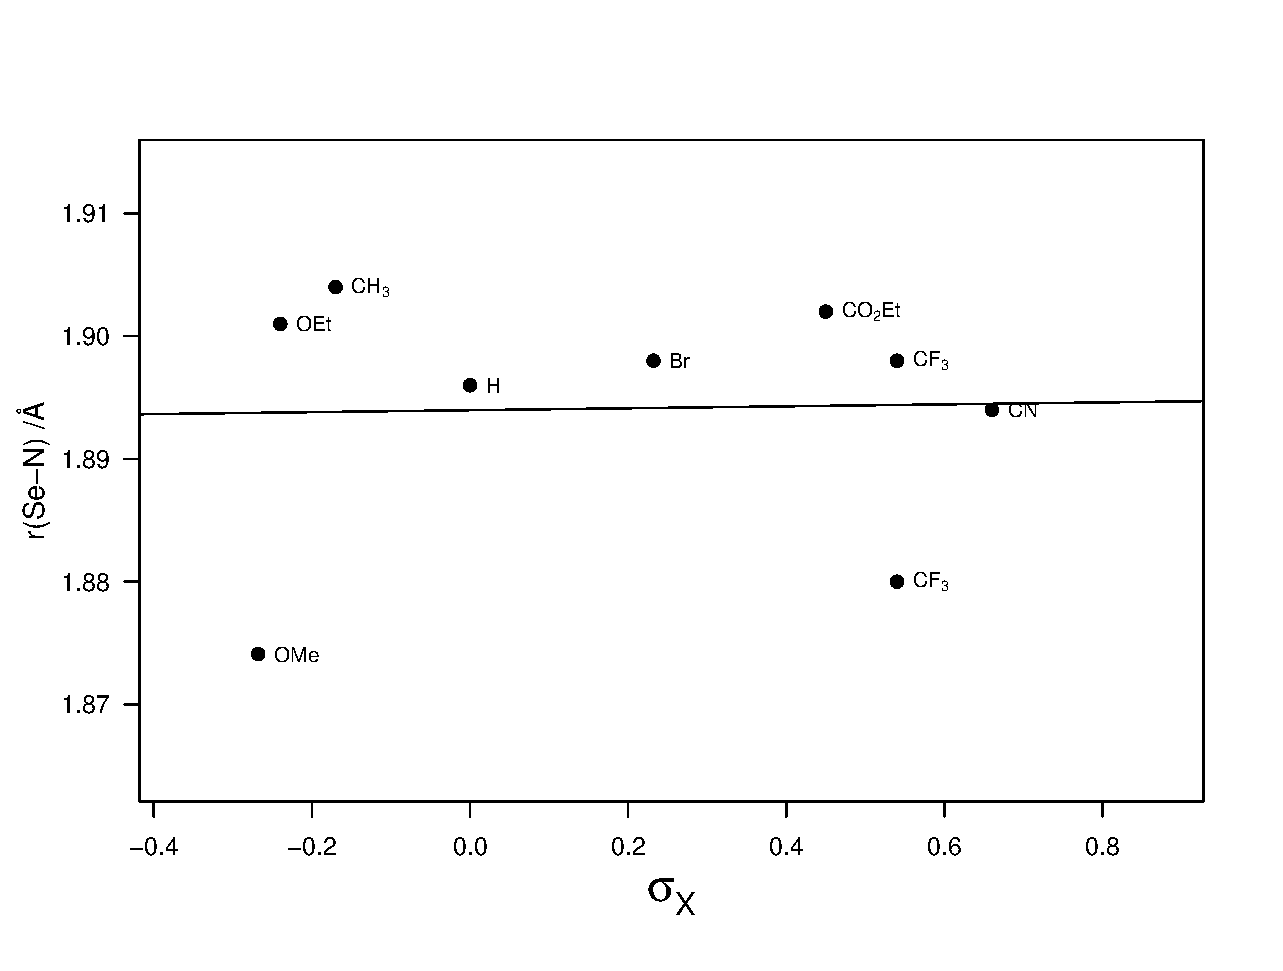
\includegraphics[width=0.9\linewidth]{Figures/hammett-endo-free.eps}
    \caption{Hammett plot of endocyclic \ce{Se-N} bond length of uncomplexed ebselen derivatives.}
    \label{fig:hammett-endo-free}
\end{figure}

The structural effects most relevant to Ch-bonding will manifest themselves in the vicinity of the selenium atom.
Of particular interest is the endocyclic \ce{Se-N} bond length, which serves as a measure of $\sigma^\star$(\ce{Se-N}) orbital occupancy, thus the degree of hyperconjugation and strength of the Ch-bond.

As can be seen in \cref{fig:hammett-endo-free}, there is practically no correlation between the electronic properties of the aryl ring and the endocyclic \ce{Se-N} bond length in crystals of the unbound ebselen derivatives.
This is not unexpected, as in all cases the crystals consist of one dimensional chains of ebselen molecules Ch-bonded to the carbonyl oxygen of the next (\cref{fig:ebs-me-packing}).
As the magnitude of the $\sigma$-hole (Ch-bond donor ability) is \emph{increased} by an electron withdrawing substituent, the Ch-bond acceptor ability of the carbonyl is \emph{decreased}.
These opposing effects appear to be approximately equal in magnitude, so cancel each other out and give a very flat and featureless Hammett plot.

\begin{figure}
  \centering
  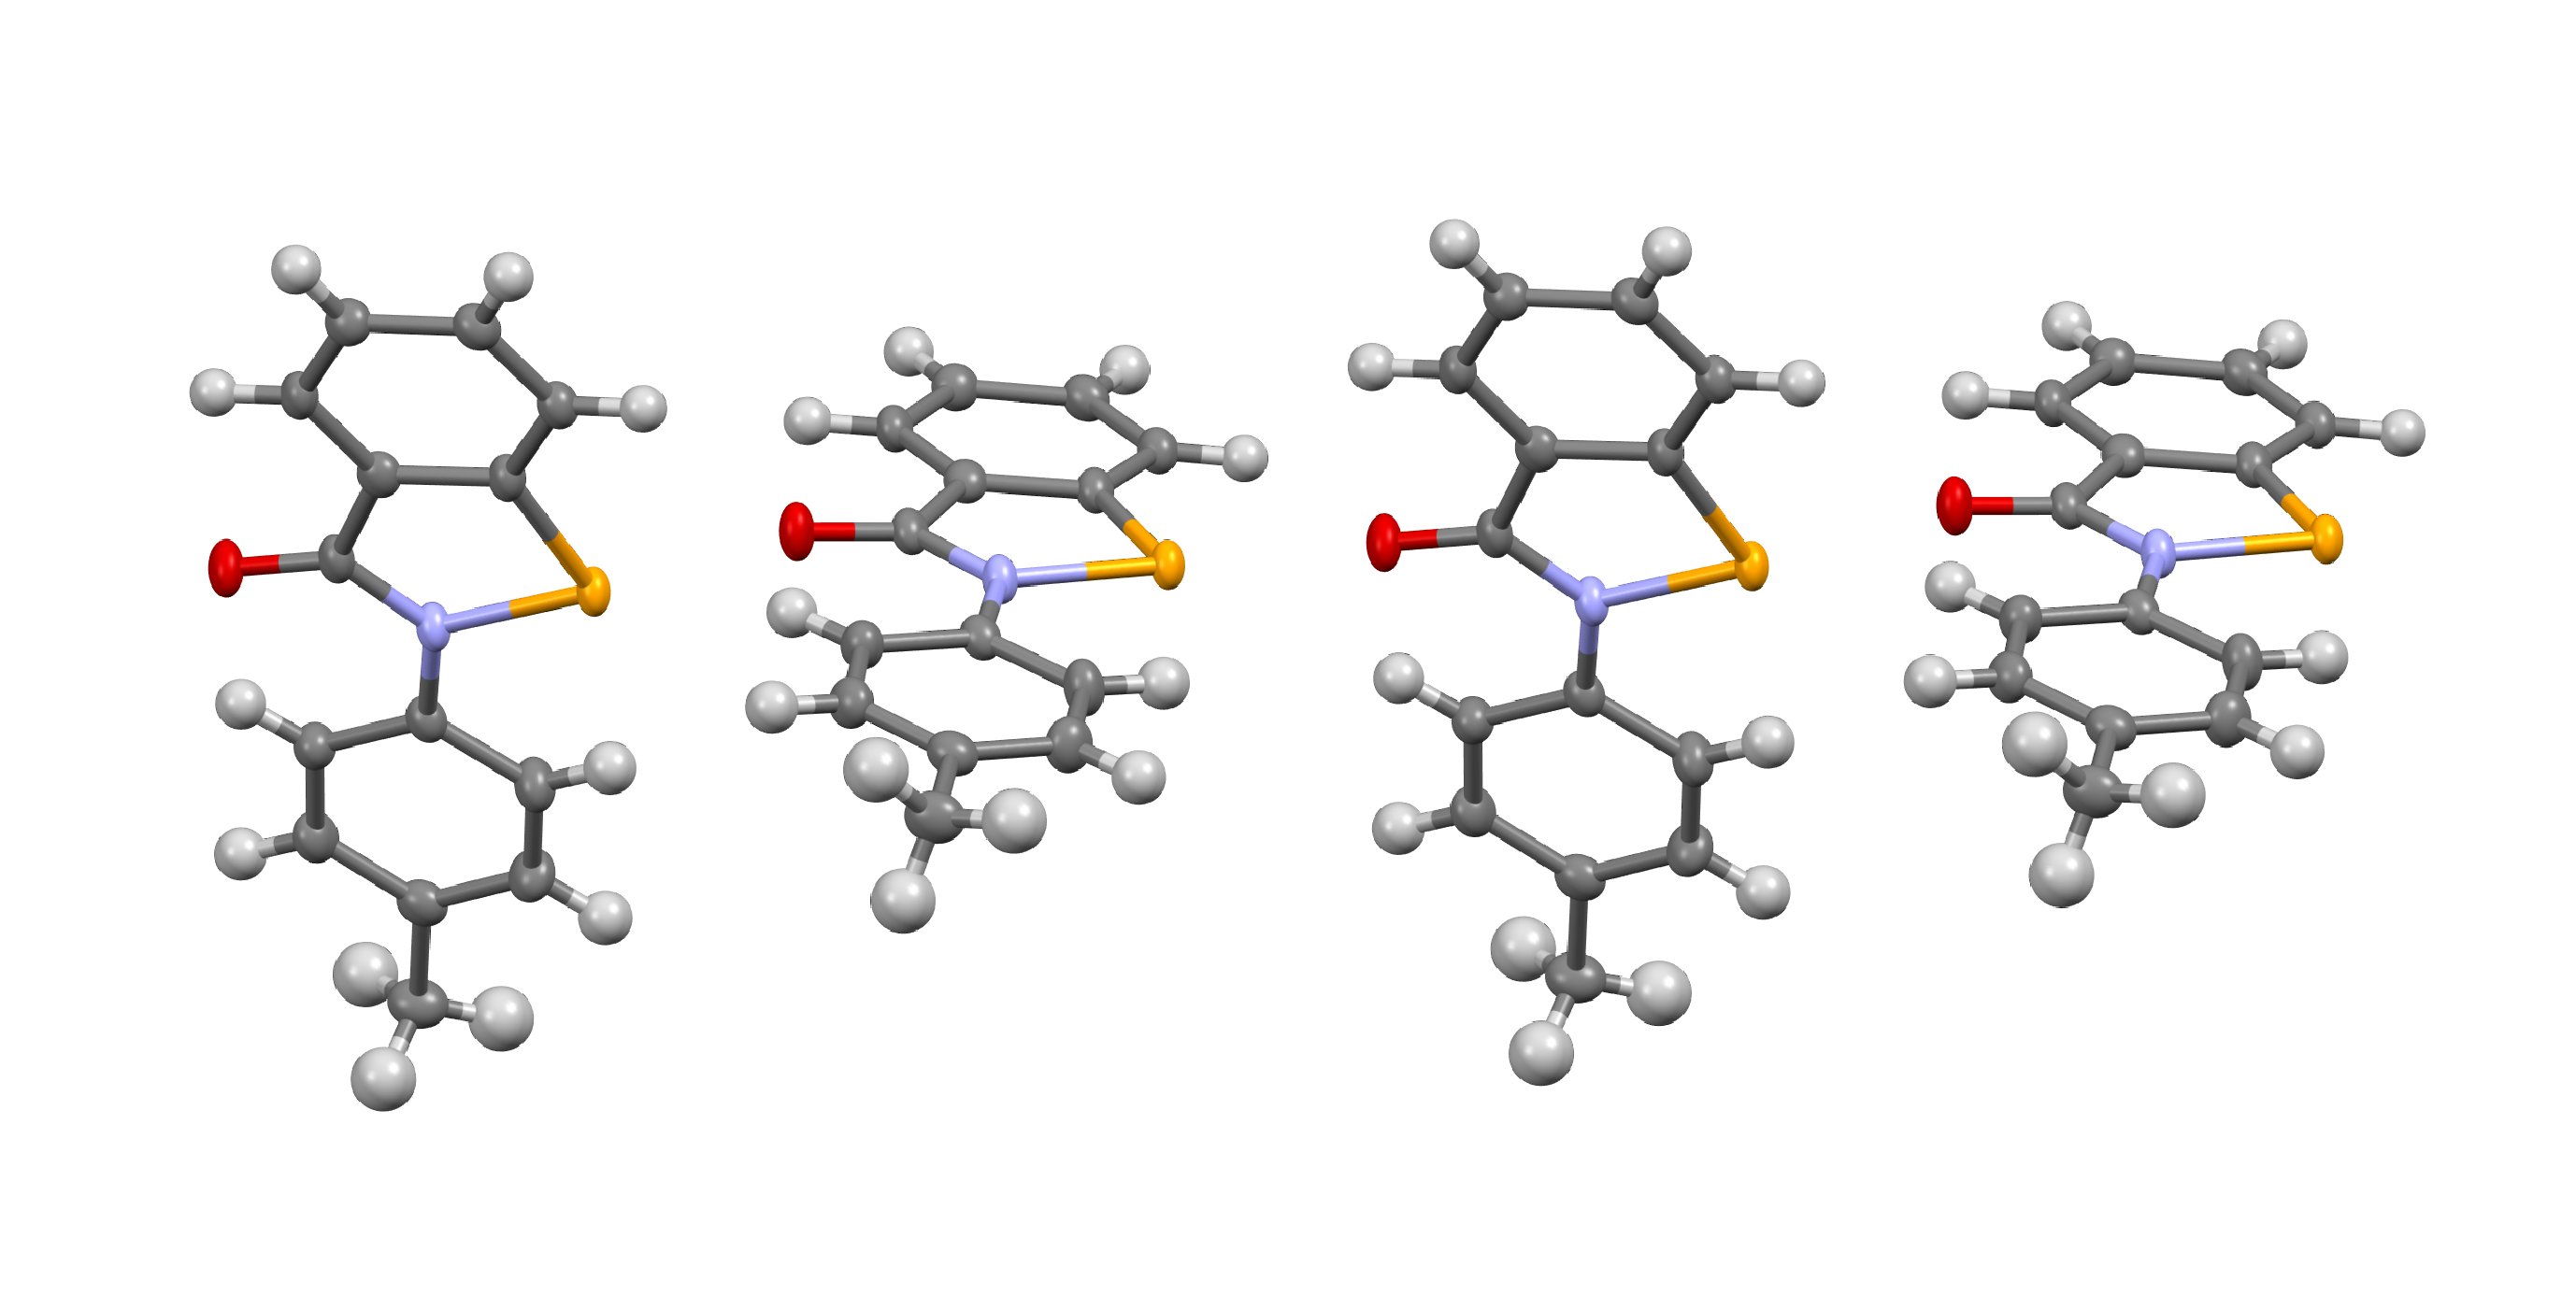
\includegraphics[width=0.6\linewidth]{Figures/ebs.me-packing.pdf}
  \caption[One dimensional chains formed by Ch-bonding between the selenium and carbonyl oxygen in \refcmpd{ebs.4me}.]{One dimensional chains formed by Ch-bonding between the selenium and carbonyl oxygen in \refcmpd{ebs.4me}. All other ebselen derivatives display a similar packing motif.}
  \label{fig:ebs-me-packing}
\end{figure}

Fortunately, inspecting the same bond length in co-crystals of ebselen derivatives and a Lewis base gives us a much clearer dependence, as can be seen in \cref{fig:hammett-dmap}, \cref{fig:hammett-pyrrol}, and \cref{fig:hammett-morph}.
This is because the Ch-bond acceptor ability is now independent of the electronic properties of the Ch-bond donor, so the \ce{Se-N} bond length is determined solely by the latter.
Linear regression analysis affords the relationship $\mathrm{r}(\ce{Se-N}) = (1.957(5) + 0.054(12) \times \sigma_{\mathrm{X}})$~\AA~with a correlation coefficient of 0.6297 for co-crystals with DMAP.

An inverse correlation can be seen in the \ce{Se\cdots N} Ch-bond length in \cref{fig:hammett-dmap}.
The gradient of the line is now negative and somewhat steeper, at $-0.15(4)$~\AA.
However the correlation coefficient is decreased to 0.5056.
The reason for this is apparent in the left hand side of the plot.
While the more strongly Ch-bonded systems (with electron withdrawing substituents) are generally very well described by the regression model, the electron rich derivatives \cmpd{ebs.4ome,ebs.4oet} vary significantly in their bond lengths.\footnote{This is also visible, though less apparent, in the plot of endocyclic bond lengths (\cref{fig:hammett-dmap}).}
Indeed, omitting these data points improves the correlation coefficient to 0.8148 while the gradient and intercept are almost unchanged at $-0.156(28)$~\AA~and $2.386(15)$~\AA~respectively, suggesting that the model is appropriate, and that there is some other effect occurring in electron rich systems.
For a further discussion of this phenomenon, see \cref{sec:z2}.

\begin{figure}
    \centering
    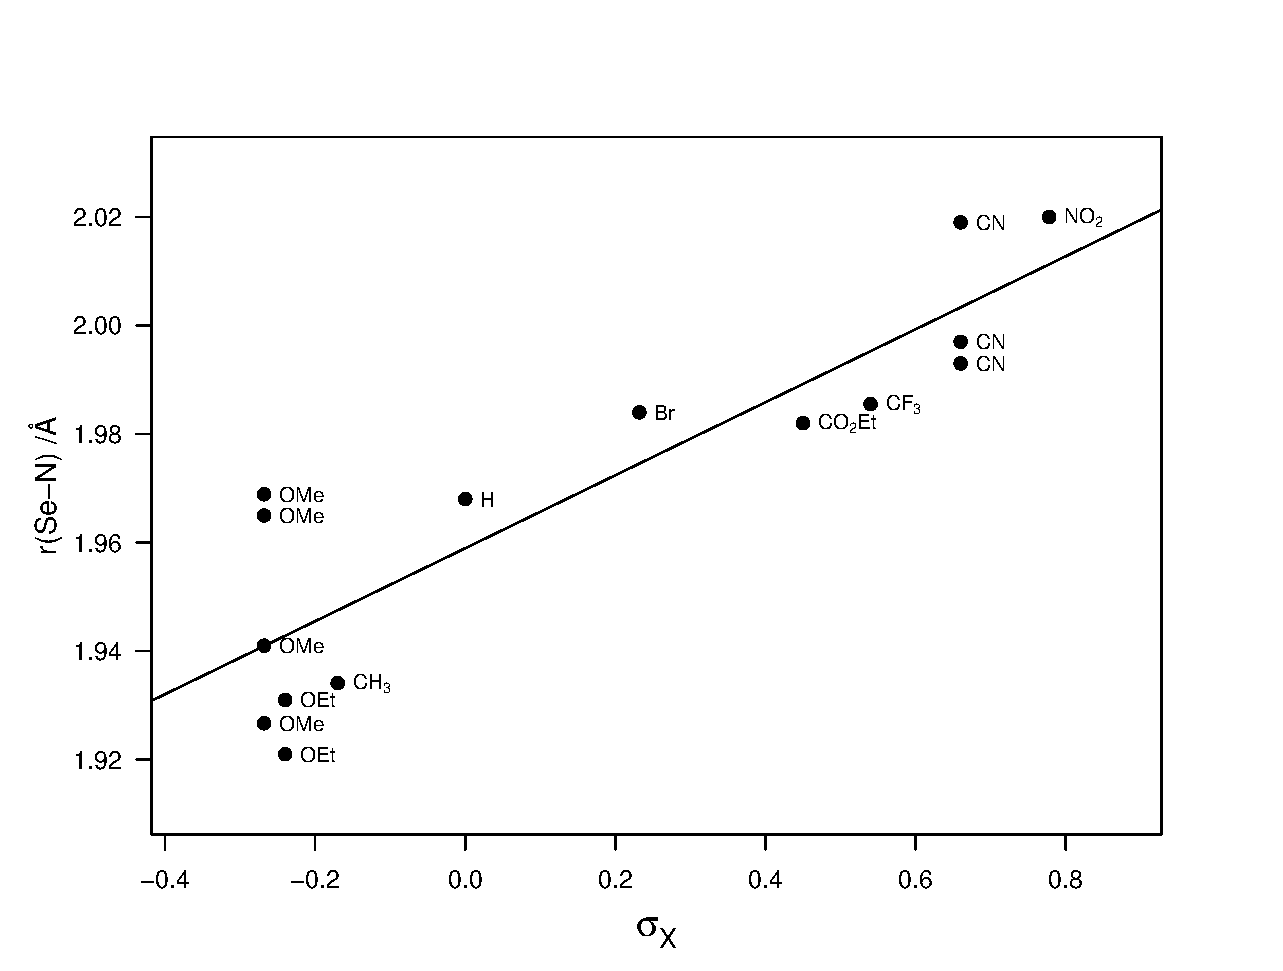
\includegraphics[width=0.9\linewidth]{Figures/hammett-endo-dmap.eps}
    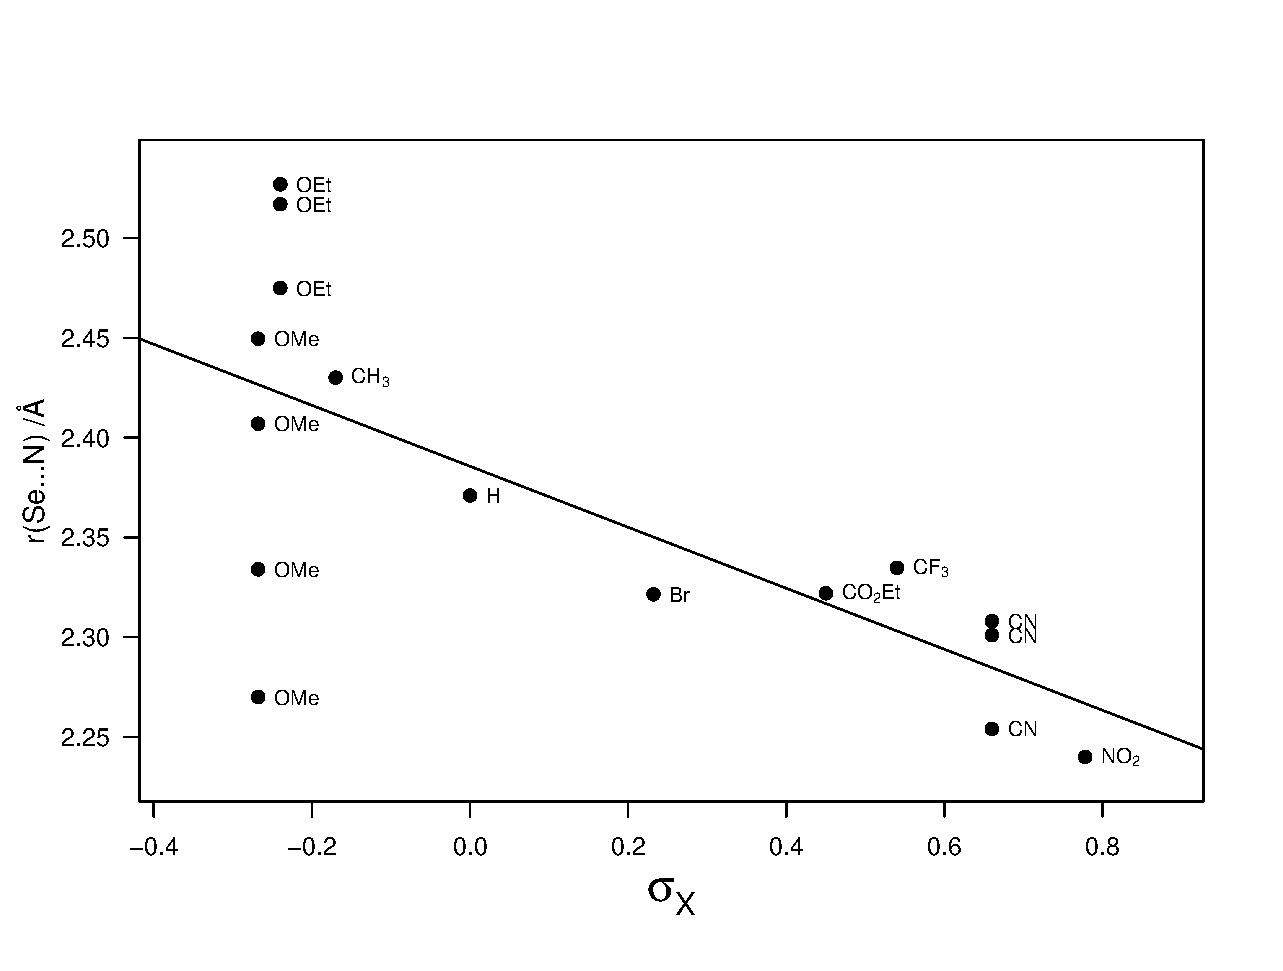
\includegraphics[width=0.9\linewidth]{Figures/hammett-dmap.eps}
    \caption[Hammett plots of endocyclic \ce{Se-N} bond length and \ce{Se\cdots N} Ch-bond length of ebselen derivatives complexed with DMAP.]{Hammett plots of endocyclic \ce{Se-N} bond length and \ce{Se\cdots N} Ch-bond length of ebselen derivatives complexed with DMAP. The lines are described by the equations $\mathrm{r}(\ce{Se-N}) = (1.959(5) + 0.067(10) \times \sigma_{\mathrm{X}})$~\AA~($R^2=0.7857$) and $\mathrm{r}(\ce{Se\cdots N}) = (2.363(17) - 0.12(4) \times \sigma_{\mathrm{X}})$~\AA~($R^2=0.4104$).}
    \label{fig:hammett-dmap}
\end{figure}

\begin{figure}
  \centering
  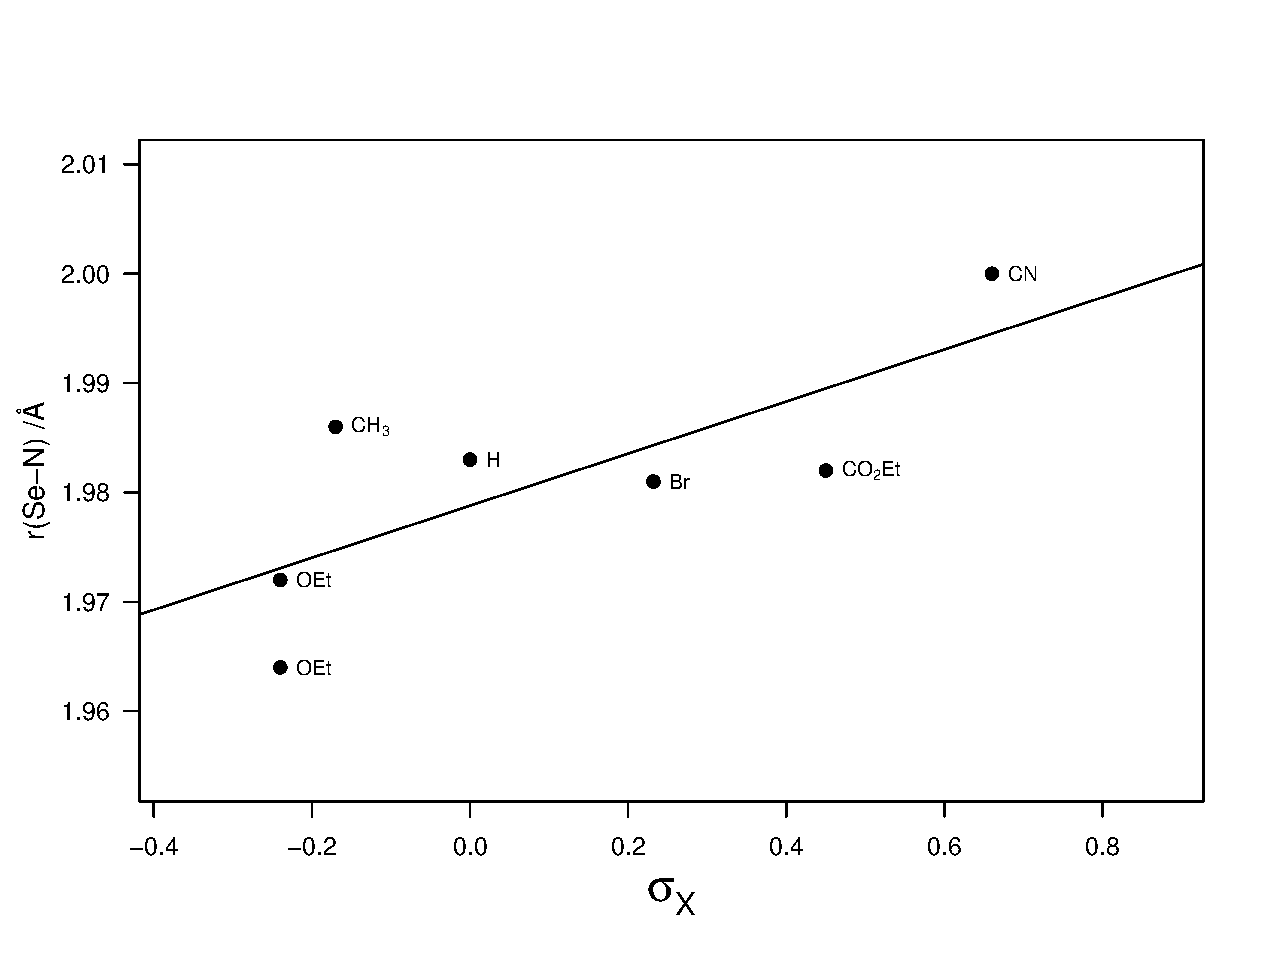
\includegraphics[width=0.9\linewidth]{Figures/hammett-endo-pyrrol.eps}
  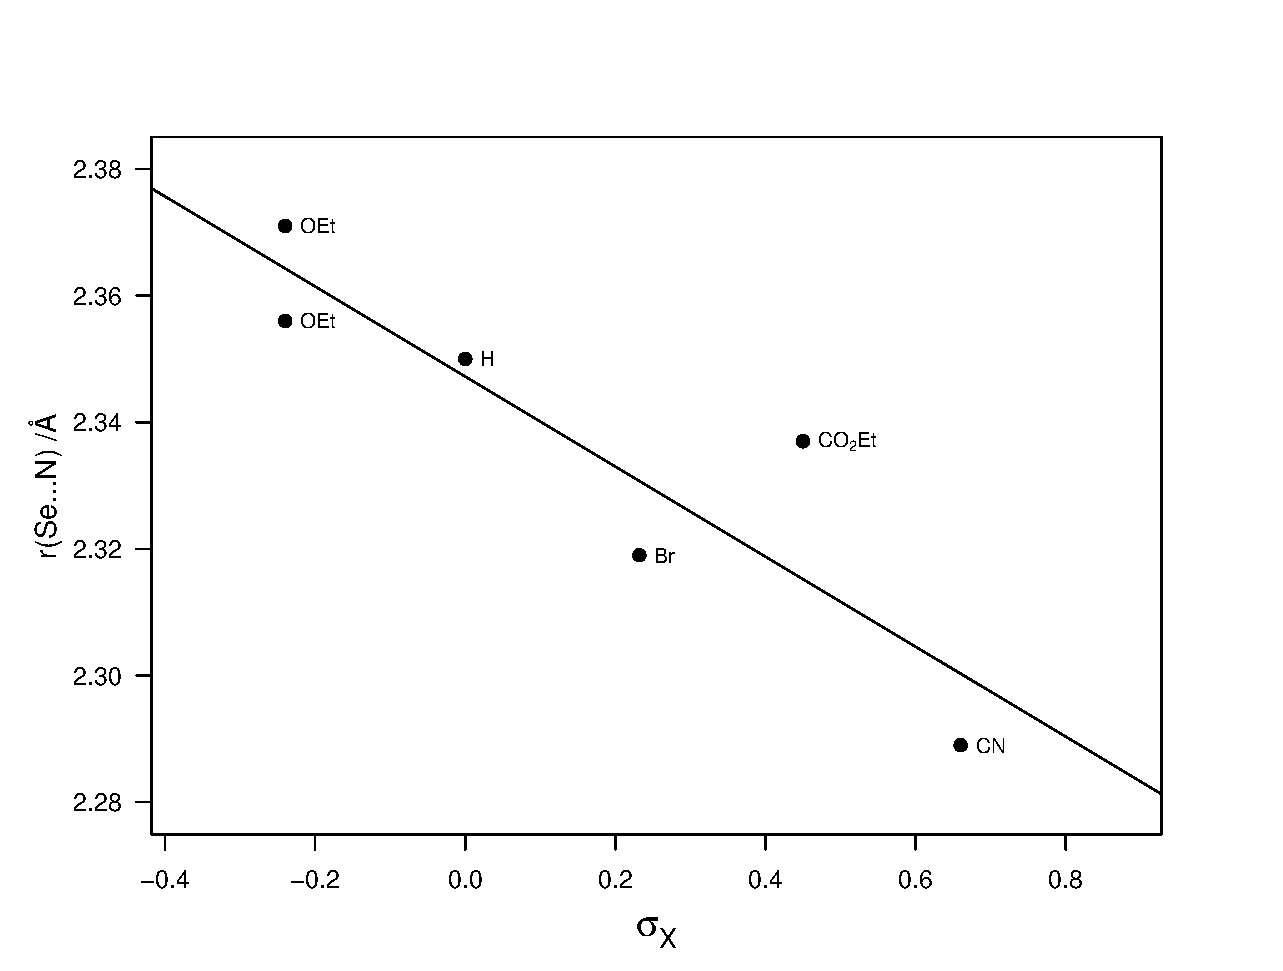
\includegraphics[width=0.9\linewidth]{Figures/hammett-pyrrol.eps}
  \caption[Hammett plots of endocyclic \ce{Se-N} bond length and \ce{Se\cdots N} Ch-bond length of ebselen derivatives complexed with \refcmpd{py.pyrrol}.]{Hammett plots of endocyclic \ce{Se-N} bond length and \ce{Se\cdots N} Ch-bond length of ebselen derivatives complexed with \refcmpd{py.pyrrol}. The lines are described by the equations $\mathrm{r}(\ce{Se-N}) = (1.9761(28) + 0.029(8) \times \sigma_{\mathrm{X}})$~\AA~($R^2=0.7828$) and $\mathrm{r}(\ce{Se\cdots N}) = (2.347(7) - 0.071(17) \times \sigma_{\mathrm{X}})$~\AA~($R^2=0.8005$)}
  \label{fig:hammett-pyrrol}
\end{figure}

\begin{figure}
  \centering
  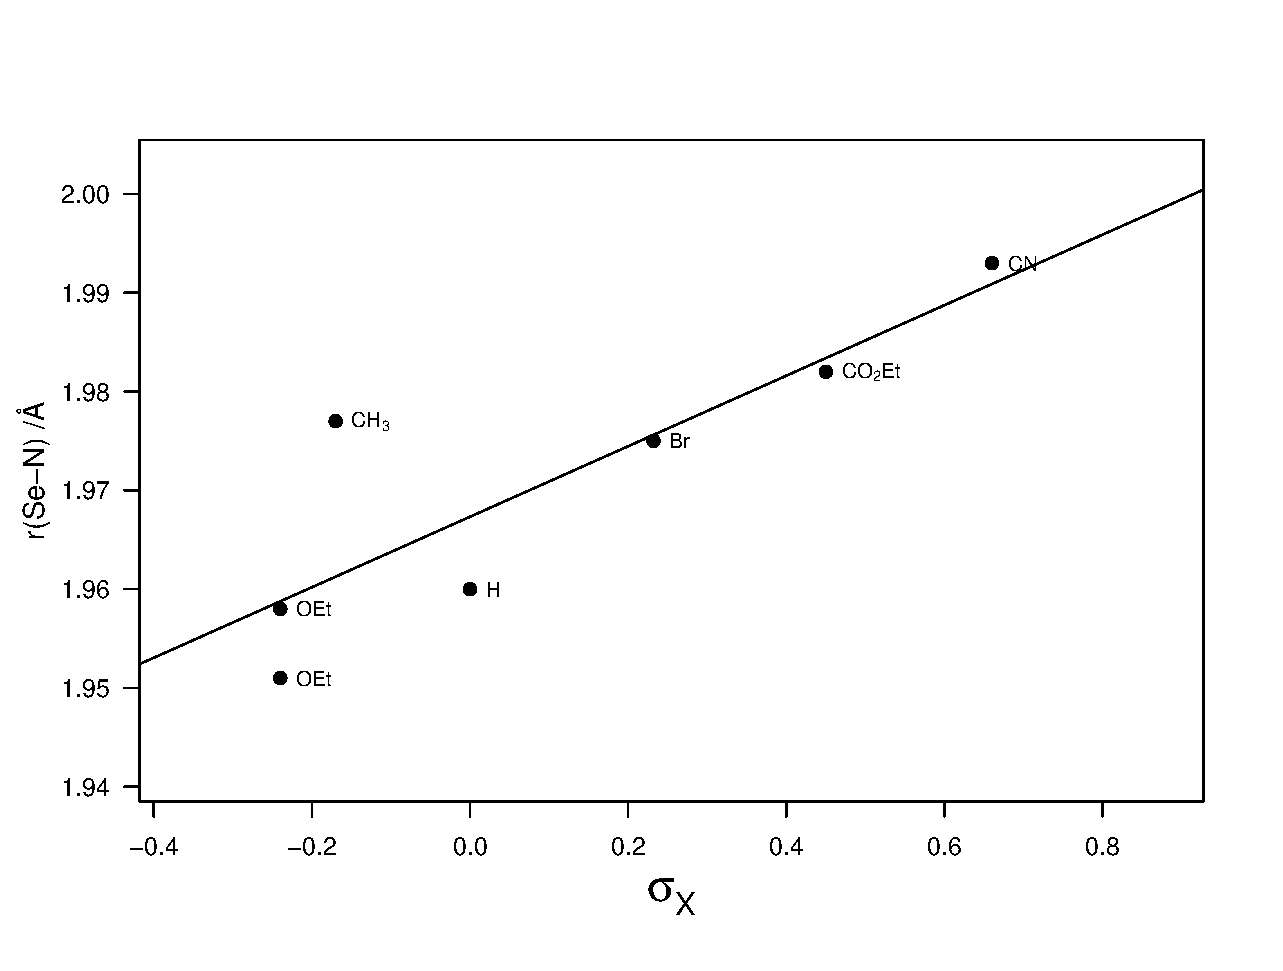
\includegraphics[width=0.9\linewidth]{Figures/hammett-endo-morph.eps}
  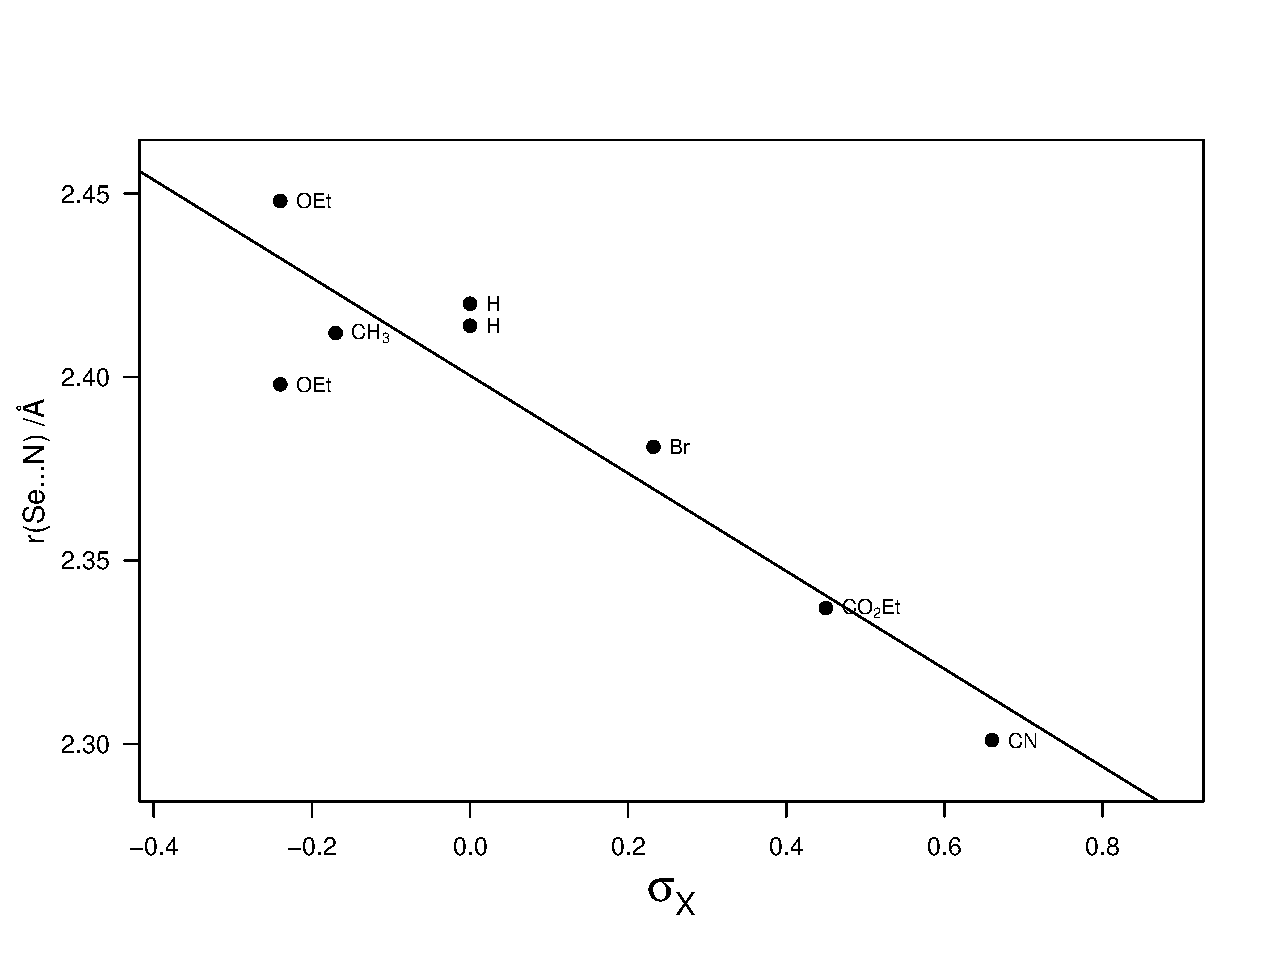
\includegraphics[width=0.9\linewidth]{Figures/hammett-morph.eps}
  \caption[Hammett plots of endocyclic \ce{Se-N} bond length and \ce{Se\cdots N} Ch-bond length of ebselen derivatives complexed with \refcmpd{py.morph}.]{Hammett plots of endocyclic \ce{Se-N} bond length and \ce{Se\cdots N} Ch-bond length of ebselen derivatives complexed with \refcmpd{py.morph}. The line is described by the equation $\mathrm{r}(\ce{Se-N}) = (1.9673(34) + 0.035(10) \times \sigma_{\mathrm{X}})$~\AA~($R^2=0.7260$) and $\mathrm{r}(\ce{Se\cdots N}) = (2.397(77) - 0.13(2) \times \sigma_{\mathrm{X}})$~\AA~($R^2=0.8708$).}
  \label{fig:hammett-morph}
\end{figure}

\begin{table}
  \caption{Linear regression results for Hammett plots in \cref{fig:hammett-dmap,fig:hammett-pyrrol,fig:hammett-morph}.}
  \begin{tabular}{lllllll}\toprule
         & \multicolumn{3}{c}{$\mathrm{r}(\ce{Se\cdots N})$} & \multicolumn{3}{c}{$\mathrm{r}(\ce{Se-N})$} \\
         \cmidrule(lr){2-4}\cmidrule(lr){5-7}
    Base            & gradient  & intercept & $R^2$ & gradient & intercept & $R^2$ \\\midrule
    DMAP            & -0.12(4)  & 2.363(17) & 0.4104& 0.067(10)& 1.959(5)  & 0.7857 \\
    \cmpd{py.pyrrol}& -0.071(17)& 2.347(7)  & 0.8005& 0.029(8) & 1.9761(28)& 0.7828 \\
    \cmpd{py.morph} & -0.13(2)  & 2.397(8)  & 0.8708& 0.035(10)& 1.9673(34)& 0.7260 \\\bottomrule 
  \end{tabular}
  \label{tab:hammett-results}
\end{table}

Hammett plots can also be constructed using the electron density parameters at the bond critical point ($\rho_\text{BCP}$ and $\nabla^2\rho_{\text{BCP}}$) of the Ch bond.
The electron density $\rho_\text{BCP}$ shows a similar trend to the bond distance ($\rho_{\text{BCP}} = (0.379(16) + 0.105(37) \times \sigma_{\mathrm{X}})$~e/\AA\textsuperscript{3}~($R^2=0.3783$)), while the Laplacian $\nabla^2\rho_{\text{BCP}}$ is more or less independent of the Hammett constant ($\nabla^2\rho_{\text{BCP}} = (2.74(13) + 0.05(29) \times \sigma_{\mathrm{X}})$~e/\AA\textsuperscript{5}~($R^2=0.002$)).
This reinforces the significance of the Laplacian not as an indicator of the strength of an interaction, but as a measure of its ionic or covalent character, which does not appear to change significantly across the range of electron demand.

\begin{figure}
  \centering
  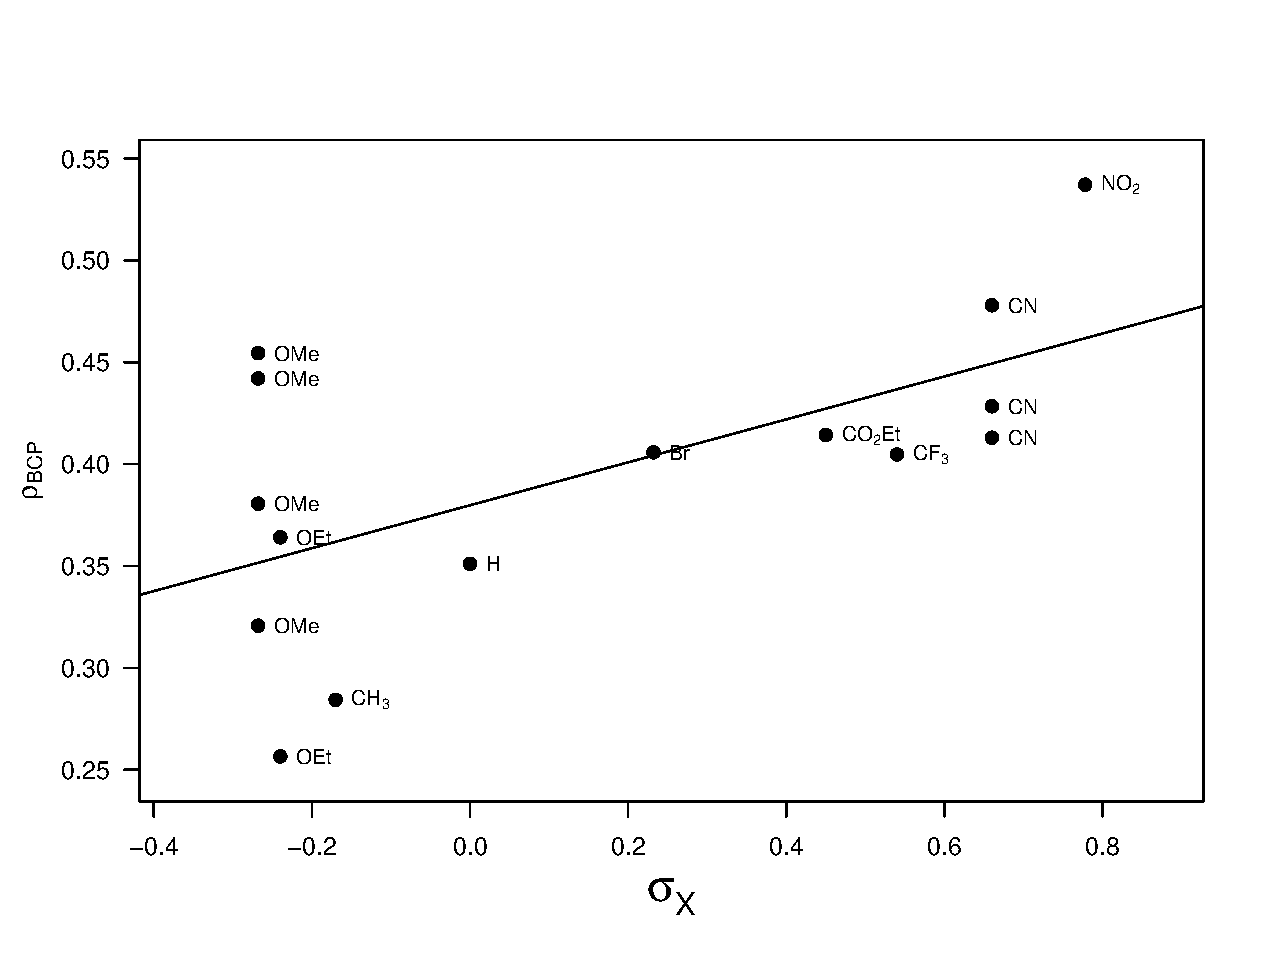
\includegraphics[width=0.9\linewidth]{Figures/hammett-rho-dmap.eps}
  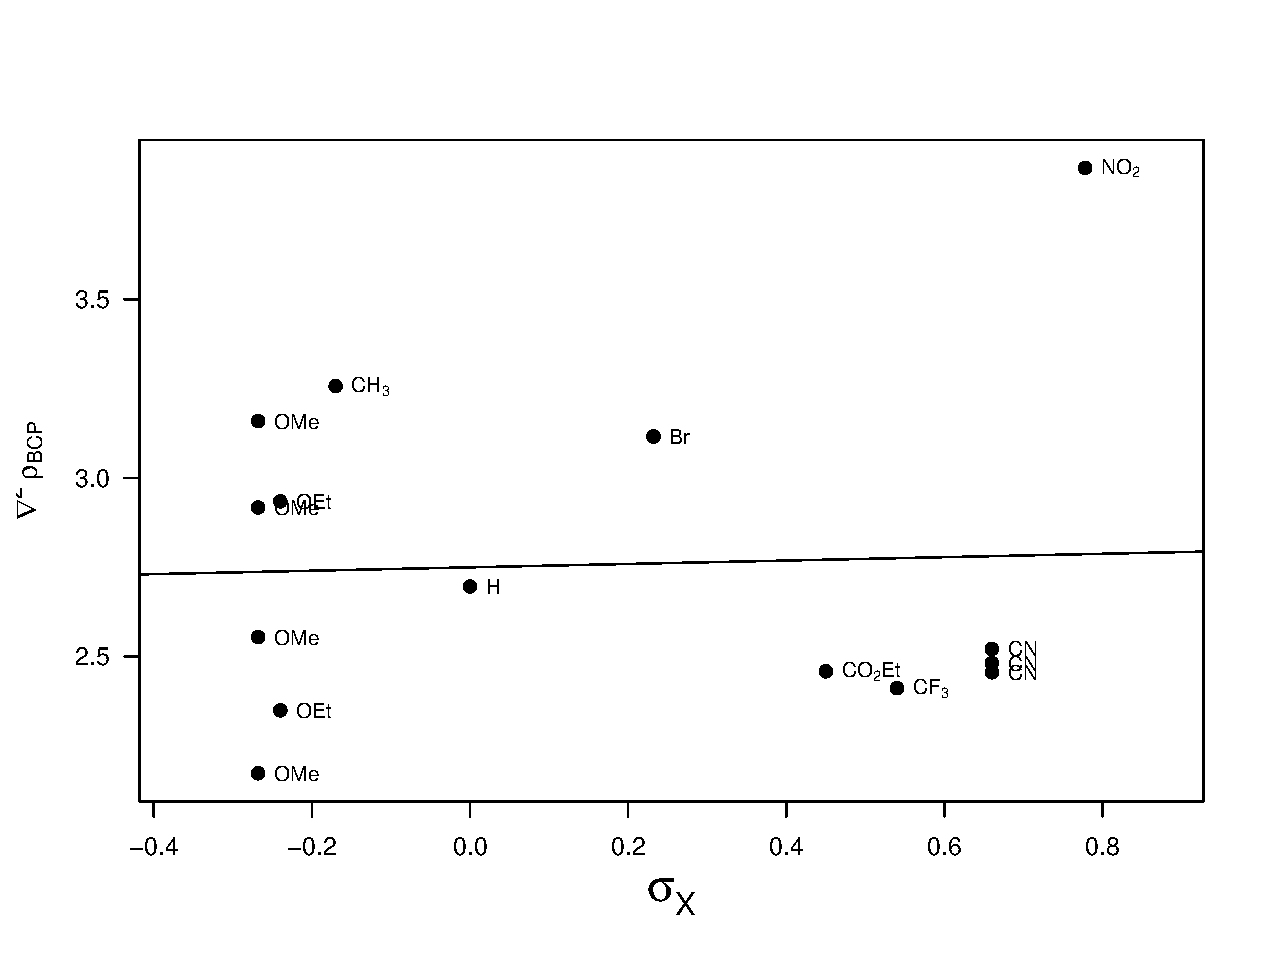
\includegraphics[width=0.9\linewidth]{Figures/hammett-lapl-dmap.eps}
  \caption[Hammett plots of QTAIM parameters $\rho_\text{BCP}$ and $\nabla^2\rho_{\text{BCP}}$ of ebselen derivatives complexed with DMAP.]{Hammett plots of QTAIM parameters $\rho_\text{BCP}$ and $\nabla^2\rho_{\text{BCP}}$ of ebselen derivatives complexed with DMAP. The line is described by the equation $\rho_{\text{BCP}} = (0.379(16) + 0.105(37) \times \sigma_{\mathrm{X}})$~e/\AA\textsuperscript{3}~($R^2=0.3783$) and $\nabla^2\rho_{\text{BCP}} = (2.74(13) + 0.05(29) \times \sigma_{\mathrm{X}})$~e/\AA\textsuperscript{5}~($R^2=0.002$)}
  \label{fig:hammett-qtaim-dmap}
\end{figure}

\begin{figure}
  \centering
  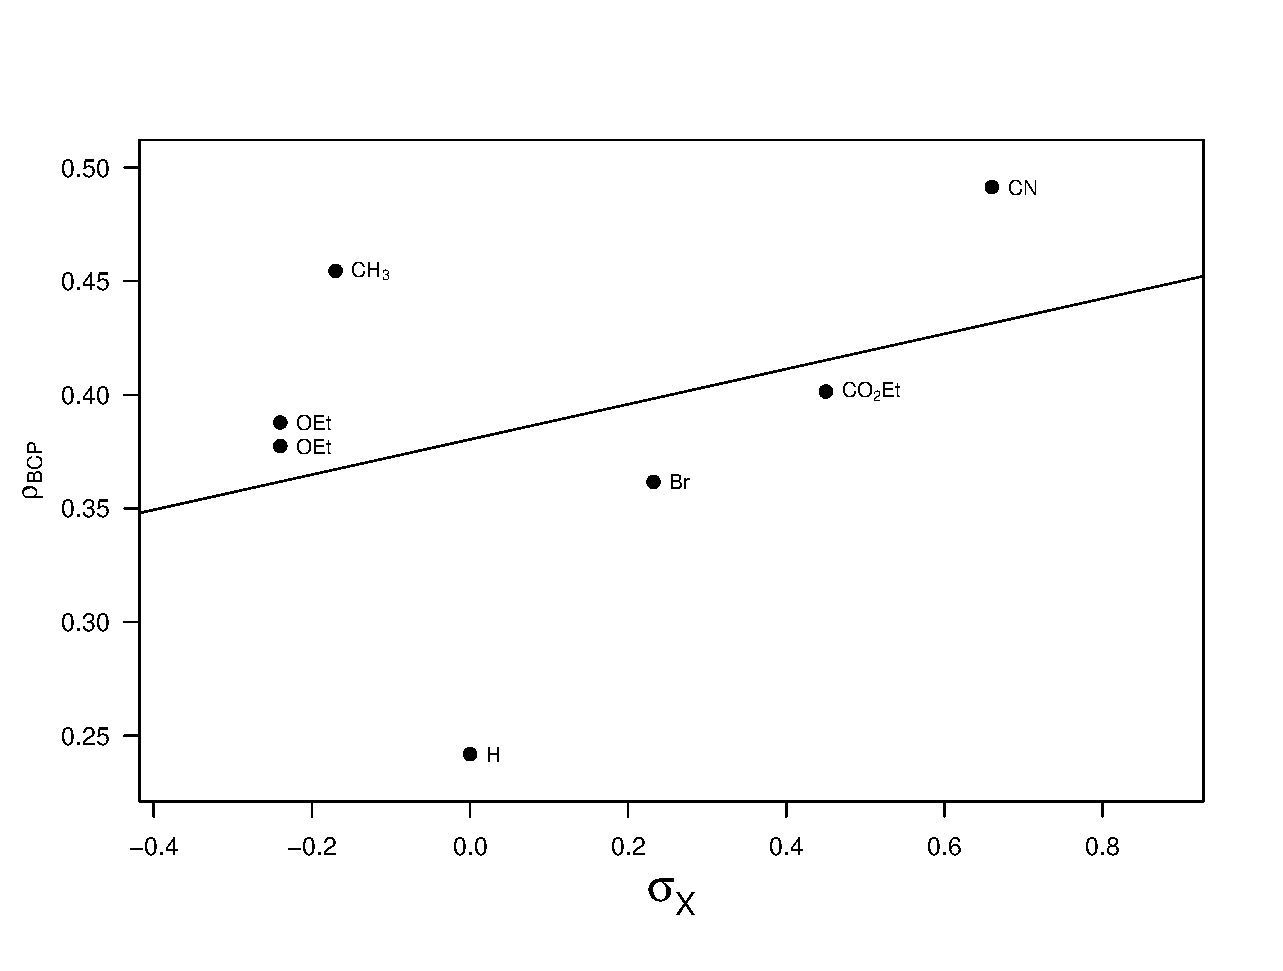
\includegraphics[width=0.9\linewidth]{Figures/hammett-rho-pyrrol.eps}
  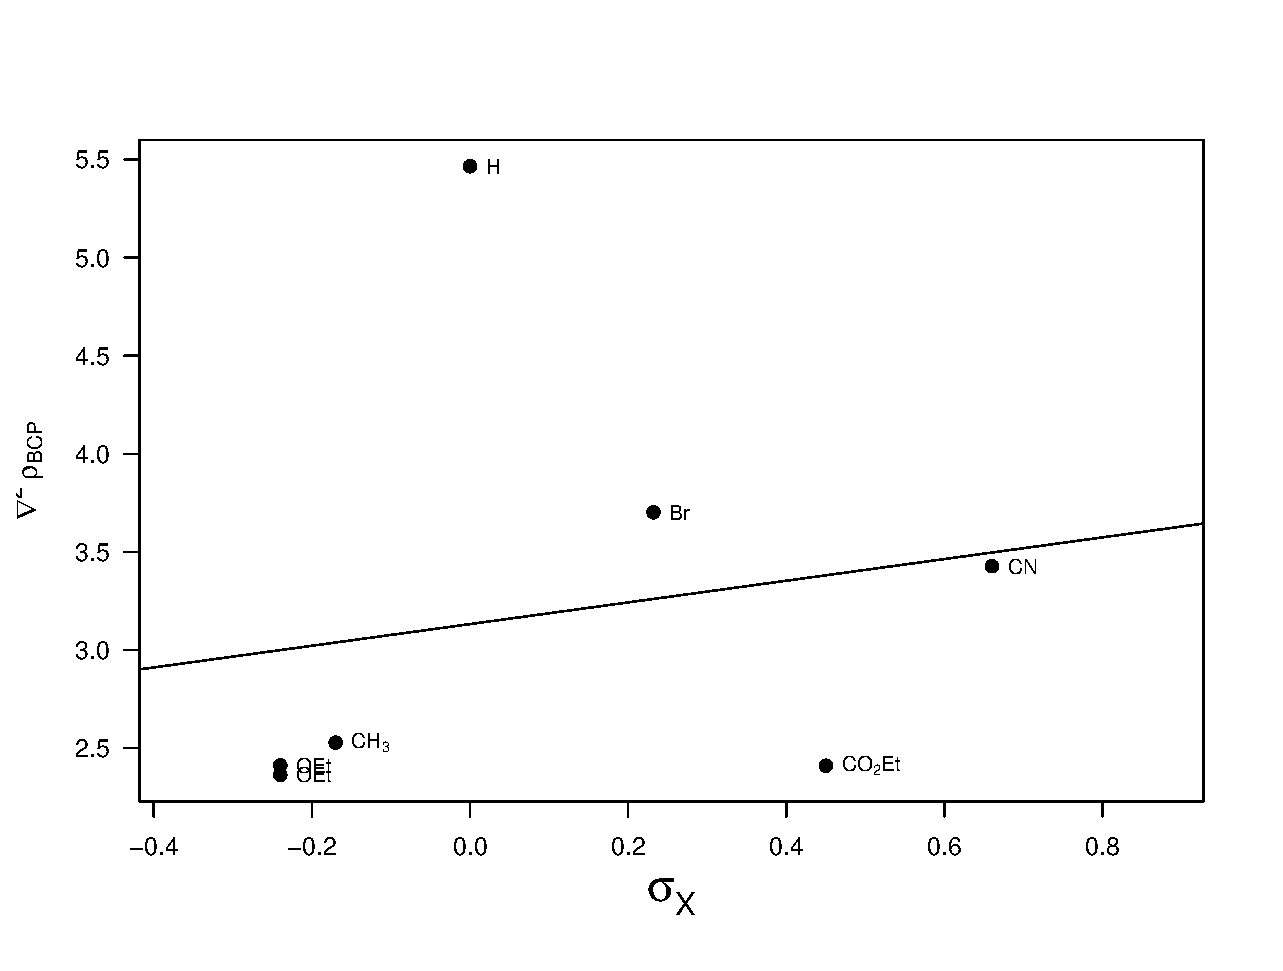
\includegraphics[width=0.9\linewidth]{Figures/hammett-lapl-pyrrol.eps}
  \caption[Hammett plots of QTAIM parameters $\rho_\text{BCP}$ and $\nabla^2\rho_{\text{BCP}}$ of ebselen derivatives complexed with \refcmpd{py.pyrrol}.]{Hammett plots of QTAIM parameters $\rho_\text{BCP}$ and $\nabla^2\rho_{\text{BCP}}$ of ebselen derivatives complexed with \refcmpd{py.pyrrol}. The line is described by the equation $\rho_{\text{BCP}} = (0.380(32) + 0.08(9) \times \sigma_{\mathrm{X}})$~e/\AA\textsuperscript{3}~($R^2=0.123$) and $\nabla^2\rho_{\text{BCP}} = (3.13(49) + 0.6(1.4) \times \sigma_{\mathrm{X}})$~e/\AA\textsuperscript{5}~($R^2=0.0299$)}
  \label{fig:hammett-qtaim-pyrrol}
\end{figure}

\begin{figure}
  \centering
  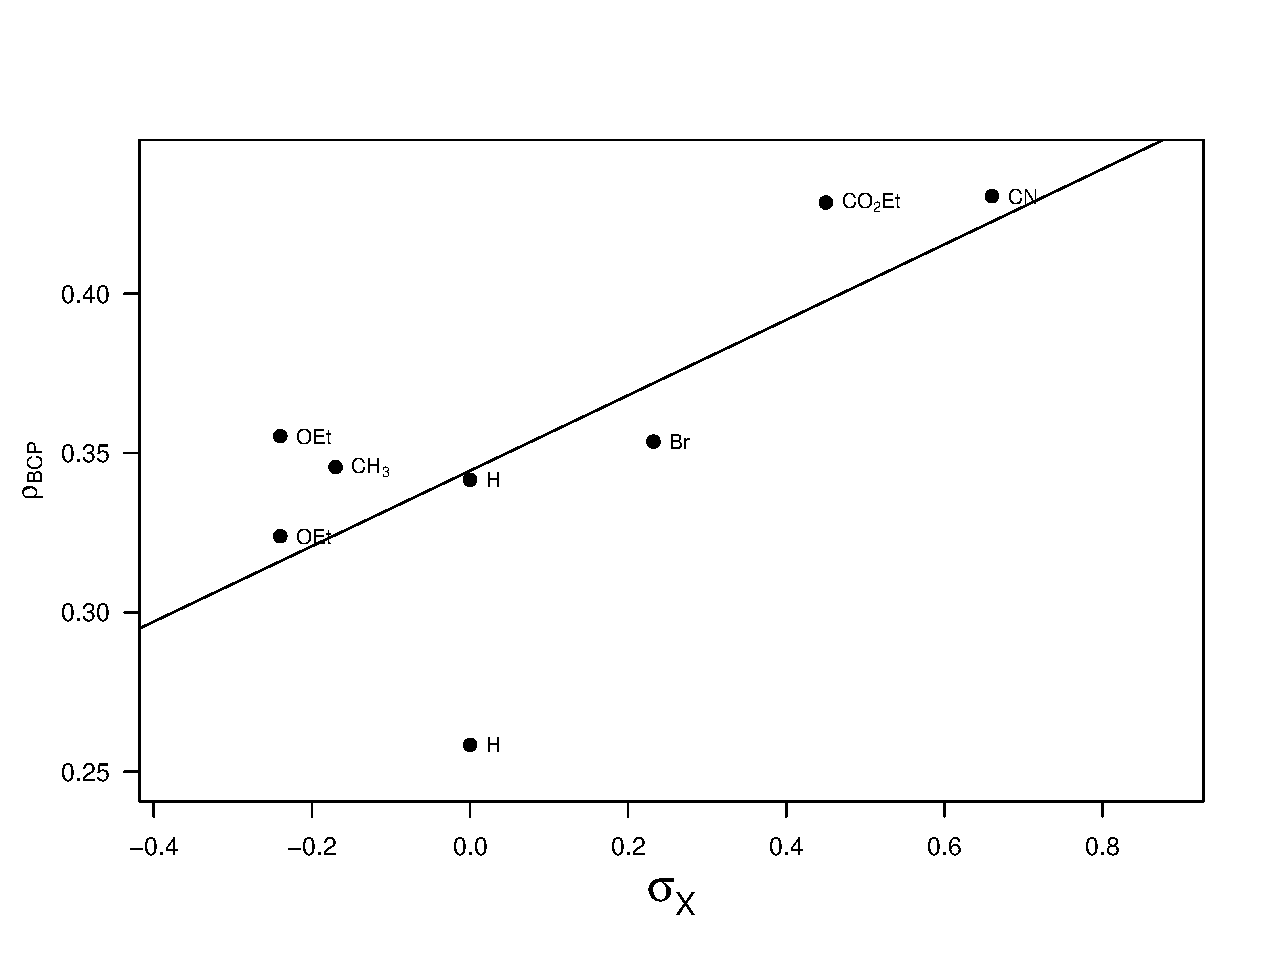
\includegraphics[width=0.9\linewidth]{Figures/hammett-rho-morph.eps}
  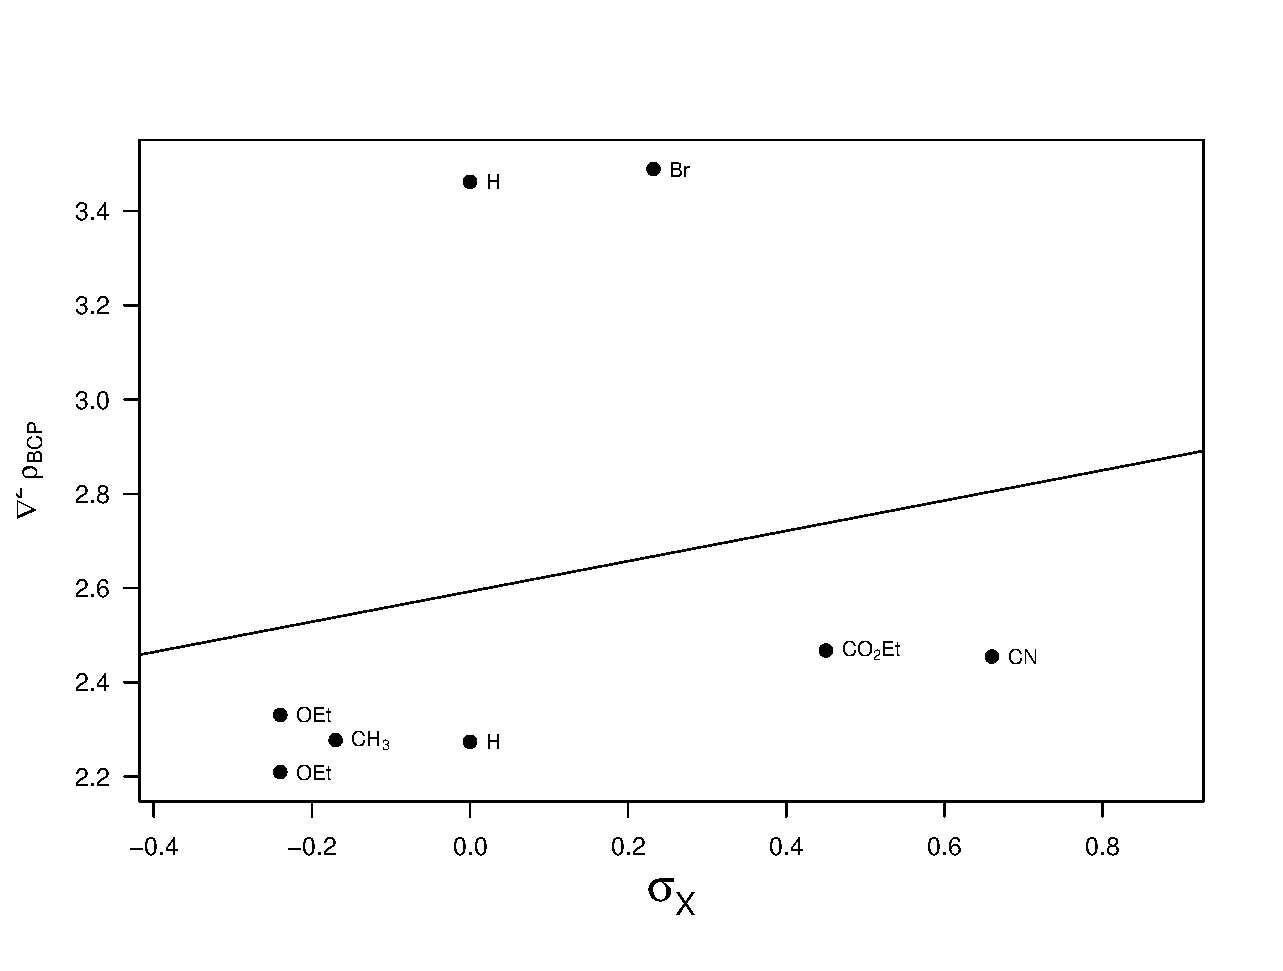
\includegraphics[width=0.9\linewidth]{Figures/hammett-lapl-morph.eps}
  \caption[Hammett plots of QTAIM parameters $\rho_\text{BCP}$ and $\nabla^2\rho_{\text{BCP}}$ of ebselen derivatives complexed with \refcmpd{py.morph}.]{Hammett plots of QTAIM parameters $\rho_\text{BCP}$ and $\nabla^2\rho_{\text{BCP}}$ of ebselen derivatives complexed with \refcmpd{py.morph}. The line is described by the equation $\rho_{\text{BCP}} = (0.344(16) + 0.12(5) \times \sigma_{\mathrm{X}})$~e/\AA\textsuperscript{3}~($R^2=0.5013$) and $\nabla^2\rho_{\text{BCP}} = (2.59(21) + 0.3(6) \times \sigma_{\mathrm{X}})$~e/\AA\textsuperscript{5}~($R^2=0.0400$)}
  \label{fig:hammett-qtaim-morph}
\end{figure}

\subsubsection{Co-crystals where \texorpdfstring{$Z^\prime=2$}{Z'=2}}
\label{sec:z2}
DFT calculations show that the vibrational mode associated with Ch-bond stretching is found at very low energy.
The force constant is 5--10~$\mu$dyne$\cdot$\AA$^{-1}$, which means that the energetic penalty associated with a 0.18~\AA~ deformation (the difference between the shortest and longest Ch-bond length) is only 0.02--0.03~kcal$\cdot$mol$^{-1}$.
Crystal packing forces (the sum of weak interactions such as C-H/$\pi$, $\pi /\pi$ and C-H/O interactions) are commonly accepted to be in the range of 1--2~kcal$\cdot$mol$^{-1}$, so it is perhaps not surprising that the Ch-bond is deformed by the crystal environment.\autocite{Dunitz1988}

That said, there are no obvious differences between the two Ch-bond environments in any of the crystals that display this effect.
We performed a solid state IR experiment to probe the crystalline environment surrounding the carbonyl, which is dependent on the Ch-bond environment due to conjugation through the amidic nitrogen (\cref{fig:ebs-4oet-dmap-ir}).

\begin{figure}
    \centering
    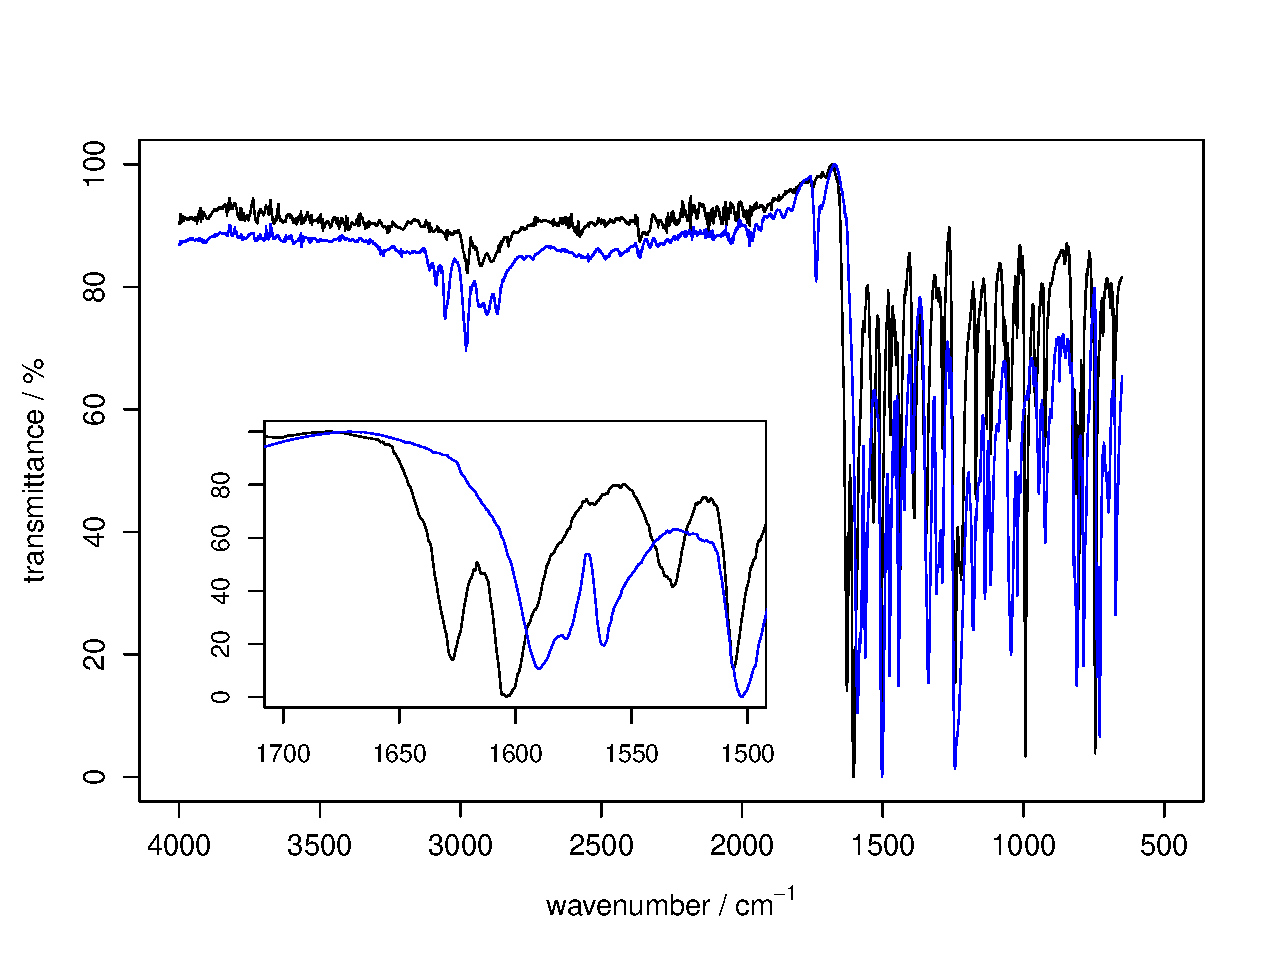
\includegraphics[width=0.9\linewidth]{Figures/ebs-4oet-dmap-ir.eps}
    \caption[Solid state IR spectrum of \refcmpd{ebs.4oet}$\cdot$DMAP.]{Solid state IR spectrum of \refcmpd{ebs.4oet}$\cdot$DMAP. The spectrum of the pure \refcmpd{ebs.4oet} is shown in gray.}
    \label{fig:ebs-4oet-dmap-ir}
\end{figure}

In the pure compound the carbonyl peak is found at approximately 1590~cm$^{-1}$ and is relatively sharp and well defined.
In the co-crystal, we observe the carbonyl peak at higher wavenumber (1610~cm$^{-1}$), due to the increased double bond character, as the $\pi$ system and oxygen lone pair are no longer involved in the Ch-bond.
This effect ostensibly outweighs the \emph{decreased} double bond character caused by the shortened Ch-bond formed between the pyridyl nitrogen and selenium (\cref{fig:ch-bond-deloc}).

\begin{figure}
    \centering
    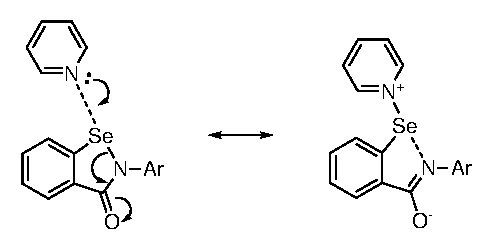
\includegraphics[scale=0.74]{Figures/ch-bond-deloc.eps}
    \caption[Resonance forms of a Ch-bonded complex with strong Lewis bases.]{Contributing resonance form of a Ch-bonded complex with strong Lewis bases. The double bond character of the carbonyl is decreased.}
    \label{fig:ch-bond-deloc}
\end{figure}

If there are truly two Ch-bonded environments, we would expect to see splitting or at least broadening of the carbonyl signal in the IR spectrum of the co-crystal.
This is not the case, meaning that either the difference is too small to be seen in the spectrum, or the two environments are actually the same, and the measured differences are a crystallographic artefact, either a manifestation of missed symmetry, disorder, or a doubled cell.

However, we do not believe this is likely, for two reasons.
Firstly, the data was of extremely high quality, and no alerts were raised in the ADDSYM routine of PLATON.
Secondly, a refinement was conducted with a tight SADI restraint on the Ch-bonds ($\sigma=0.0001$), which forced them to adopt the same length of approximately 1.949~\AA.
This increased the R-factor by 1.2\%, and significant residual density was visible where the pyridyl nitrogen had been displaced.
Furthermore, removal of the restraint recovered the original model, ruling out the possibility of a false minimum.

Solid state NMR of the co-crystal was also used to investigate the crystalline environment.
A sample of \cmpd{ebs.4ome}$\cdot$DMAP was first characterised by single crystal x-ray diffraction, which confirmed the polymorph and structural parameters (\cref{fig:ebs-4ome-dmap-xray}).

\begin{figure}
  \centering
  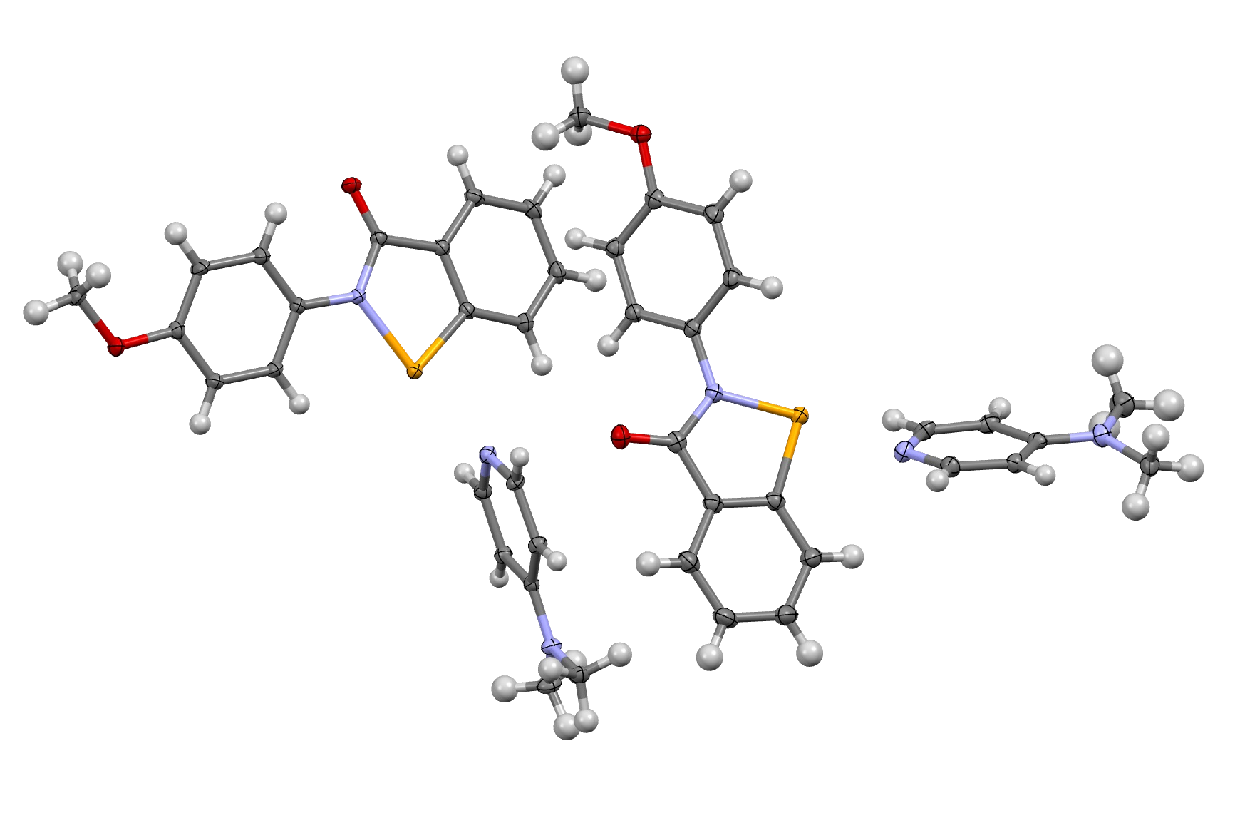
\includegraphics[width=0.8\linewidth]{Figures/ebs-4ome-dmap-xray.pdf}
  \caption[Single crystal x-ray structure of \refcmpd{ebs.4ome}\texorpdfstring{$\cdot$}{.}DMAP.]{Single crystal x-ray structure of \refcmpd{ebs.4ome}$\cdot$DMAP, displaying the two systems in the asymmetric unit.}
  \label{fig:ebs-4ome-dmap-xray}
\end{figure}

The bulk material was then crushed and homogenised, and characterised by powder x-ray diffraction.
The measured powder pattern was in excellent agreement with the pattern calculated from the single crystal data (\cref{fig:ebs-4ome-dmap-pdx}), indicating good phase purity.

\begin{figure}
    \centering
    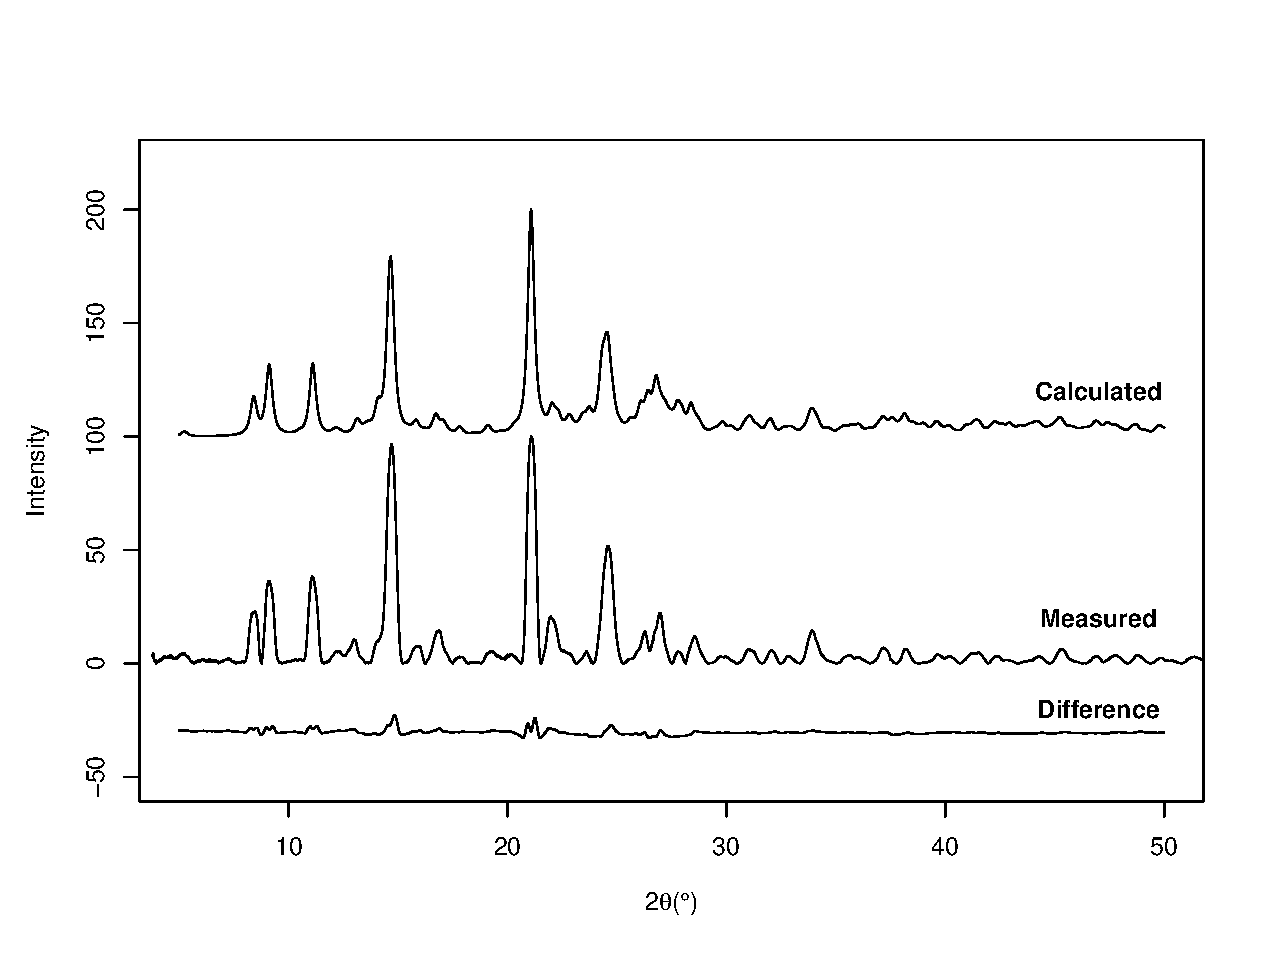
\includegraphics[width=0.9\linewidth]{Figures/ebs-4ome-dmap-pdx.eps}
    \caption{Calculated vs measured powder diffraction pattern for \refcmpd{ebs.4ome}$\cdot$DMAP.}
    \label{fig:ebs-4ome-dmap-pdx}
\end{figure}

Spectra were then acquired using a 400~MHz instrument and triple resonance MAS room temperature probe tuned to \ce{^1H}, \ce{^{13}C} and  \ce{^{77}Se}.
\ce{^1H}--\ce{^{13}C} or \ce{^1H}--\ce{^{77}Se} cross polarisation was used for signal enhancement, and a spin frequency of 10~kHz was used in most cases.

\ce{CDCl3} solution spectra of the complex were also obtained on a 500~MHz instrument.
The \ce{^1H} and \ce{^1H}--\ce{^{13}C} HSQC spectra (\cref{fig:ebs-4ome-dmap-sol}) were used to unambiguously assign the \ce{^{13}C} spectrum.

\begin{figure}
    \centering
    \begin{subfigure}[t]{\linewidth}
    \centering
    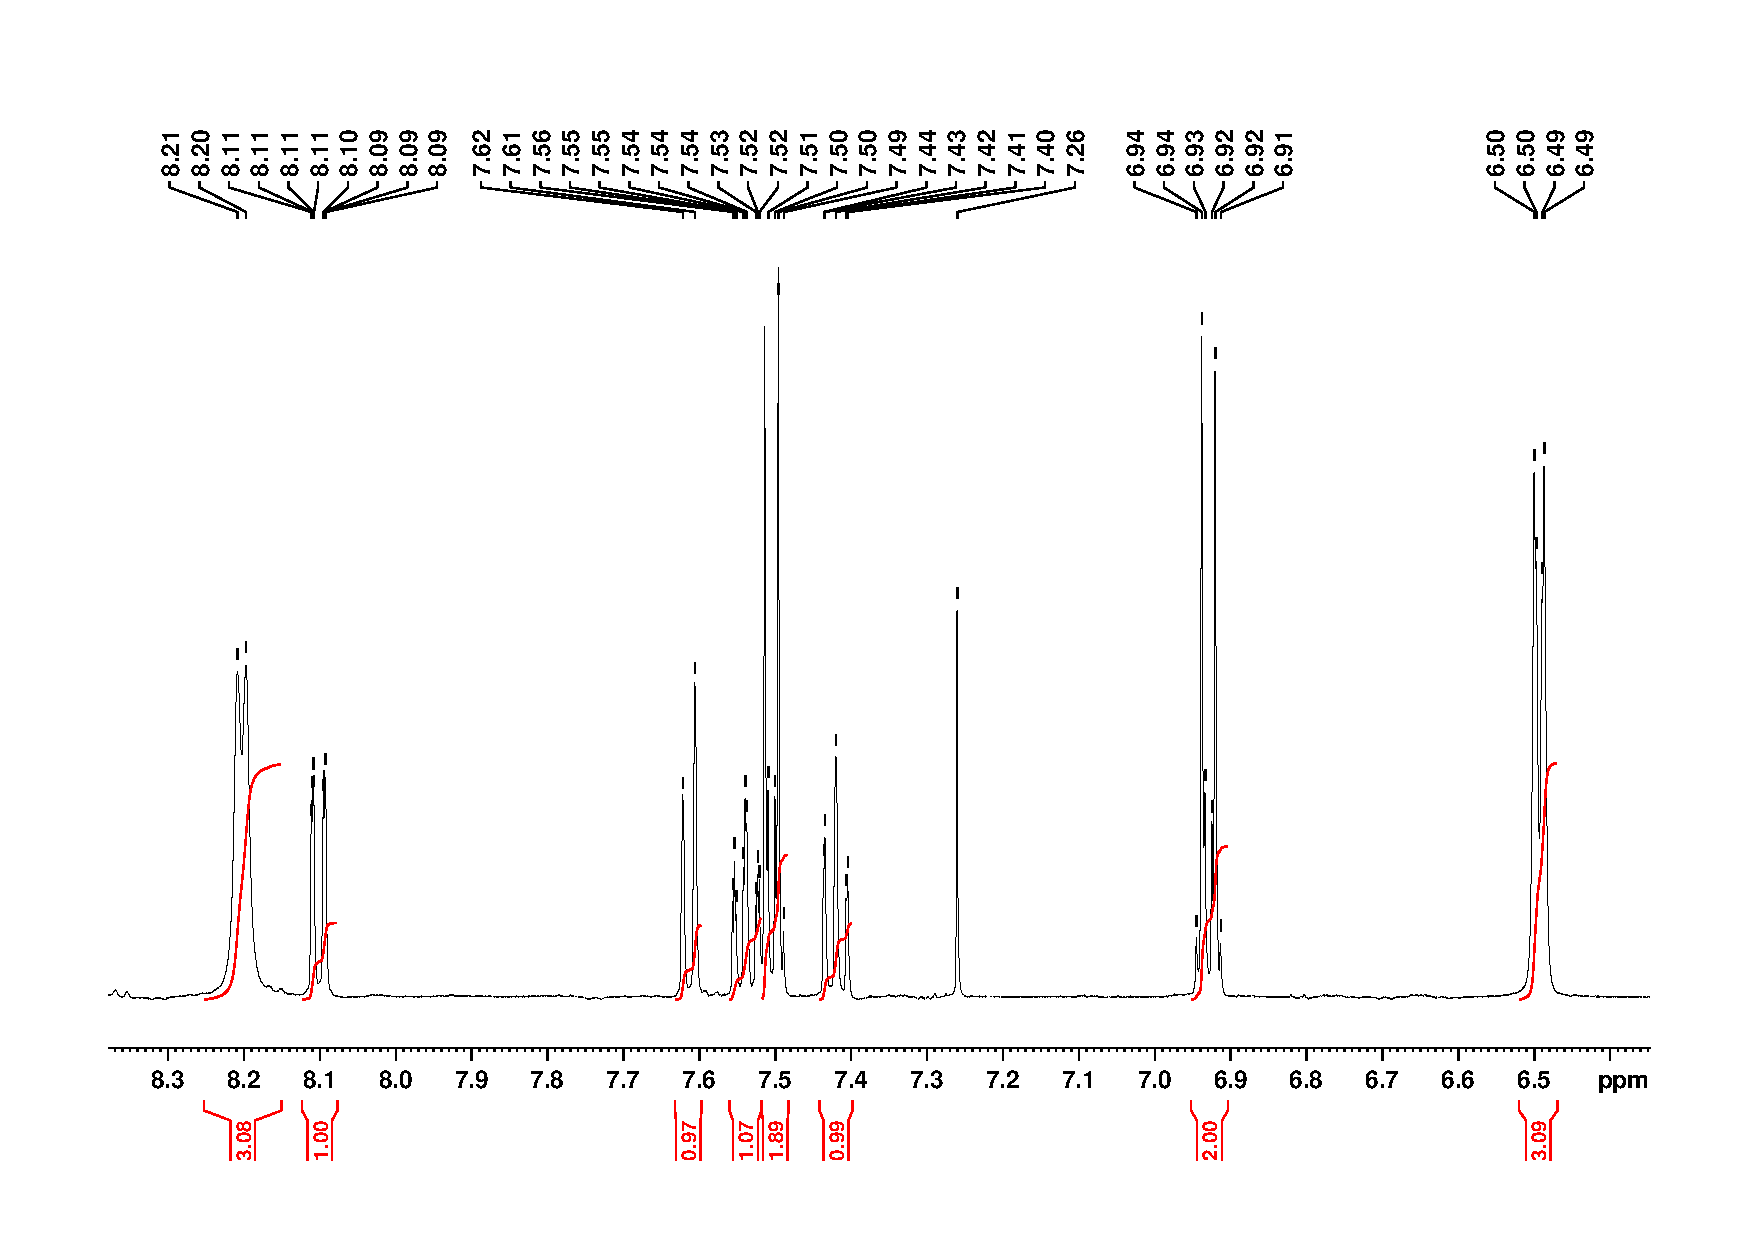
\includegraphics[width=0.9\linewidth]{Figures/ebs-4ome-dmap-sol-1h.pdf}
    \caption{Solution \ce{^1H} spectrum of \refcmpd{ebs.4ome}$\cdot$DMAP}
    \label{fig:ebs-4ome-dmap-sol-1h}
    \end{subfigure}

    \begin{subfigure}[t]{\linewidth}
    \centering
    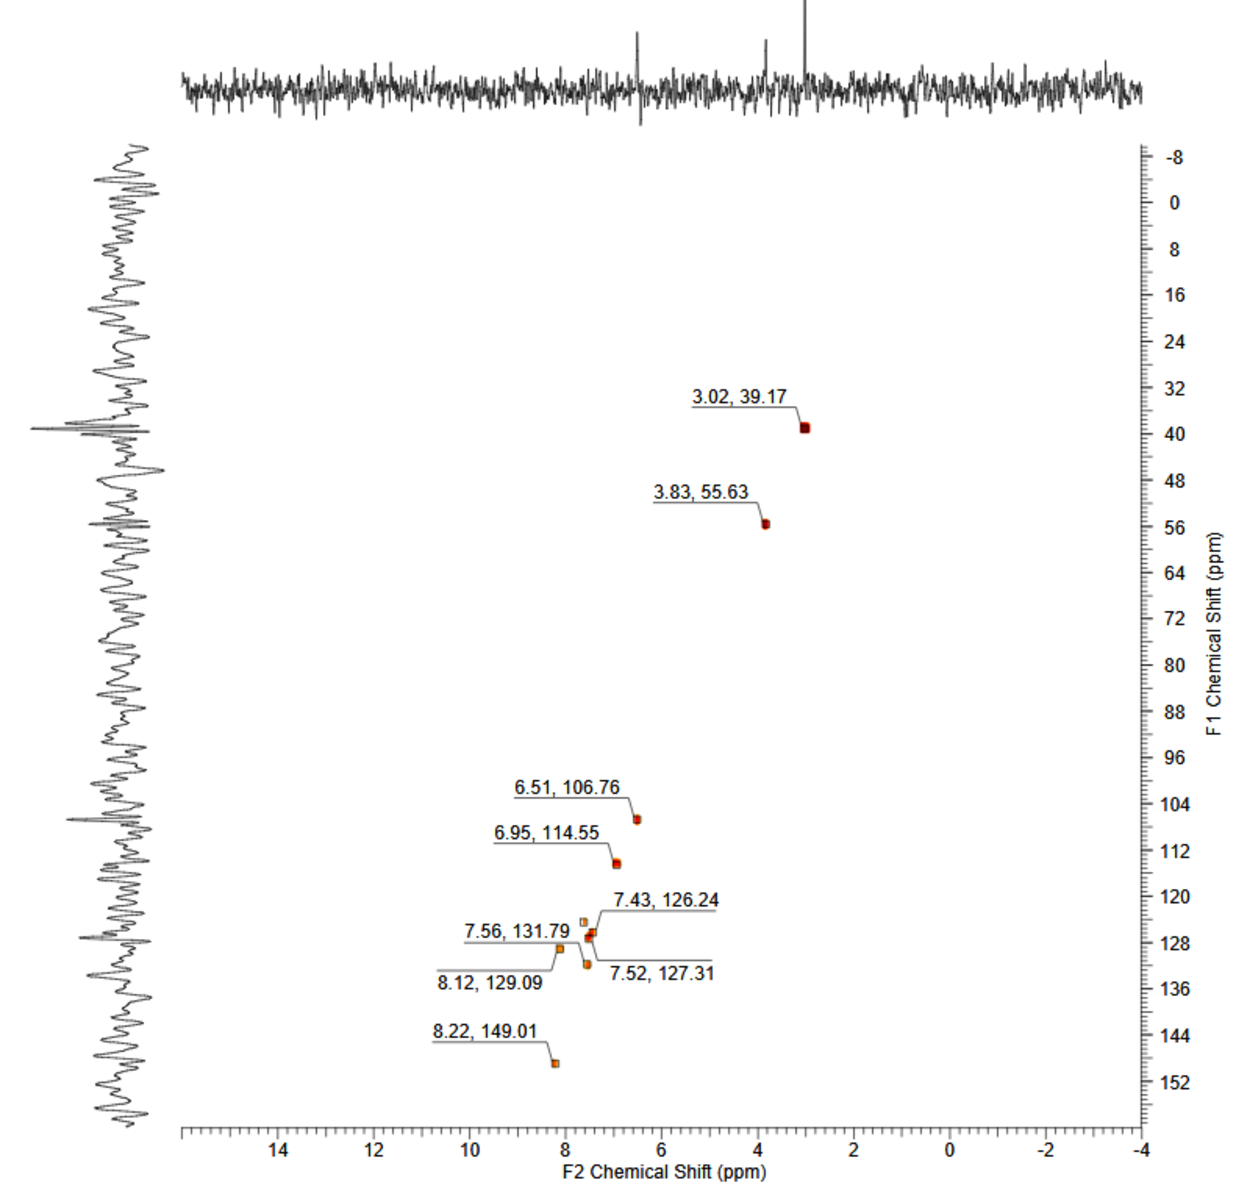
\includegraphics[width=0.75\linewidth]{Figures/ebs-4ome-dmap-sol-hsqc.pdf}
    \caption{Solution \ce{^1H}-\ce{^{13}C} HSQC spectrum of \refcmpd{ebs.4ome}$\cdot$DMAP}
    \label{fig:ebs-4ome-dmap-sol-hsqc}
    \end{subfigure}
    \caption[Solution NMR spectra of \refcmpd{ebs.4ome}\texorpdfstring{$\cdot$}{.}DMAP.]{}
    \label{fig:ebs-4ome-dmap-sol}
\end{figure}

The aromatic region of the solid state \ce{^{13}C} spectrum is shown in \cref{fig:cpmas-sol-13c}, overlaid with the corresponding solution spectrum\footnote{The \ce{^{13}C} spectrum was referenced to adamantane at $\delta$\ce{CH} $= 29.45$~ppm and $\delta$\ce{CH2} $= 38.48$~ppm.\autocite{Morcombe2003}}.
Good agreement is observed for all signals, with some interesting phenomena visible in the solid state spectrum.
Firstly, the signal at 138.62~ppm corresponding to C8 is split into a 1:1:1 triplet, possibly due to coupling to the spin 1 \ce{^{14}N} nucleus adjacent.
However this is not observed for the C7 signal, nor any signals in the pyridyl ring.
Secondly, shoulders can be seen on the C15/C19 and C16/C18 signals.
This indicates that the crystalline environment surrouding each DMAP is different, which provides further evidence that there are indeed two systems in the asymmetric unit.
The relatively poor resolution of the solid state \ce{^{13}C} NMR spectrum limits further analysis, particularly of the C1 signal which is obscured by several other signals.

\begin{figure}
    \centering
    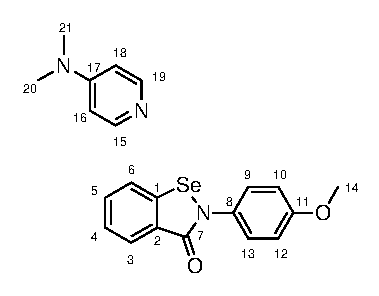
\includegraphics[scale=0.74]{Figures/numbering.eps}

    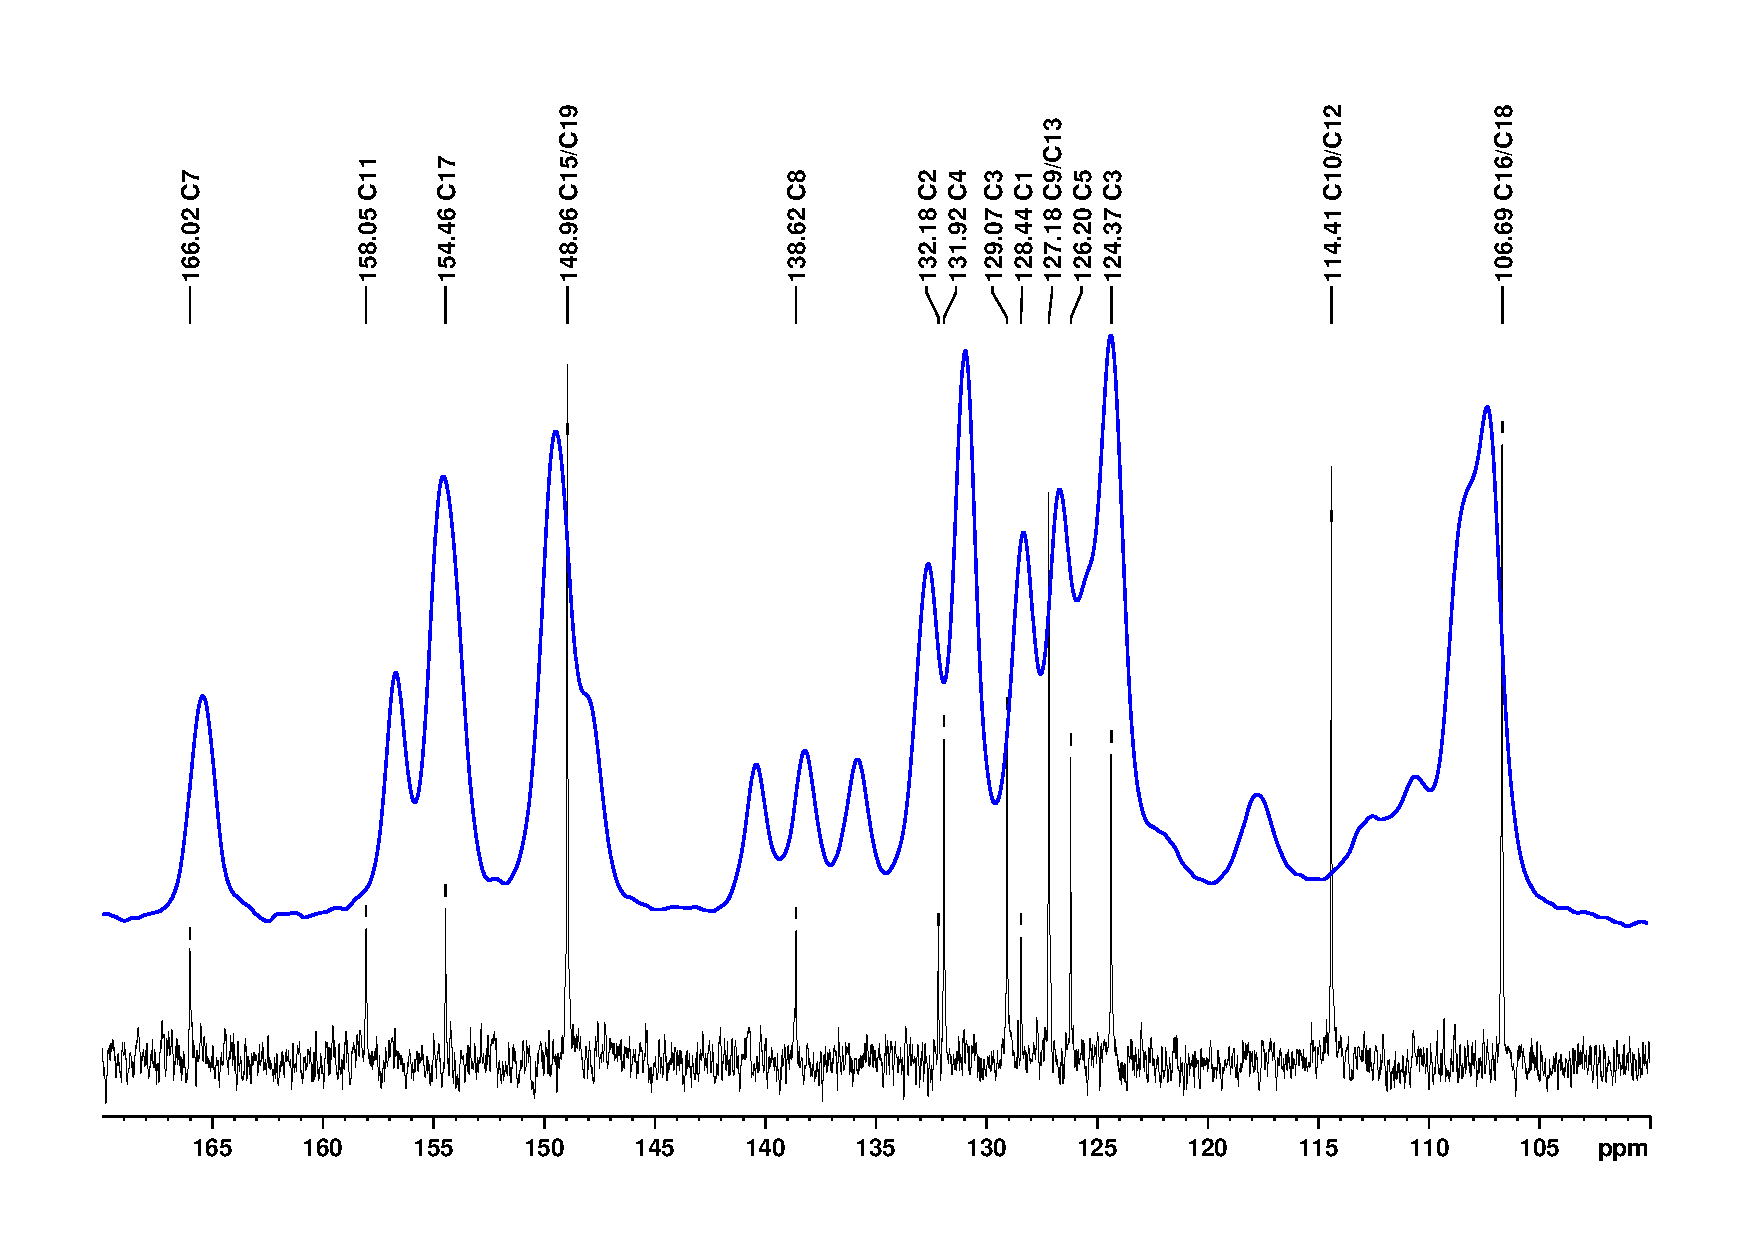
\includegraphics[width=\linewidth]{Figures/ebs-4ome-dmap-cpmas-sol-13c.pdf}
    \caption[Solid state \ce{^{13}C}-NMR spectrum of \refcmpd{ebs.4ome}$\cdot$DMAP.]{Solid state \ce{^{13}C}-NMR spectrum of \refcmpd{ebs.4ome}$\cdot$DMAP (blue) overlaid on solution spectrum of the same (black). Signals are assigned according to the numbering scheme above.}
    \label{fig:cpmas-sol-13c}
\end{figure}

To conclusively demonstrate that there are two systems in the asymmetric unit we conducted a solid state \ce{^{77}Se} NMR experiment, which is shown in \cref{fig:cpmas-sol-77se}.\footnote{The \ce{^{77}Se} spectrum was referenced to diphenyl diselenide at $\delta=463$~ppm.}
In solution, the \ce{^{77}Se} resonance is found around 900~ppm relative to dimethylselenide ($\delta=0$~ppm), and appears as one singlet due to the averaging of all environments.
In the solid phase, the spectrum is significantly more complex, primarily due to chemical shift anisotropy which manifests as spinning sidebands.
The true anisotropic chemical shifts can only be discerned by varying the MAS spinning speed, which changes the spacing of the sidebands while leaving the parent signals in the same place.
Spinning at 12~kHz instead of 10~kHz showed that the signals at 834.69 and 867.02~ppm are the true isotropic chemical shifts, and the fact that there are two signals show that there are indeed two Ch-bonded systems in the asymmetric unit.

\begin{figure}
    \centering
    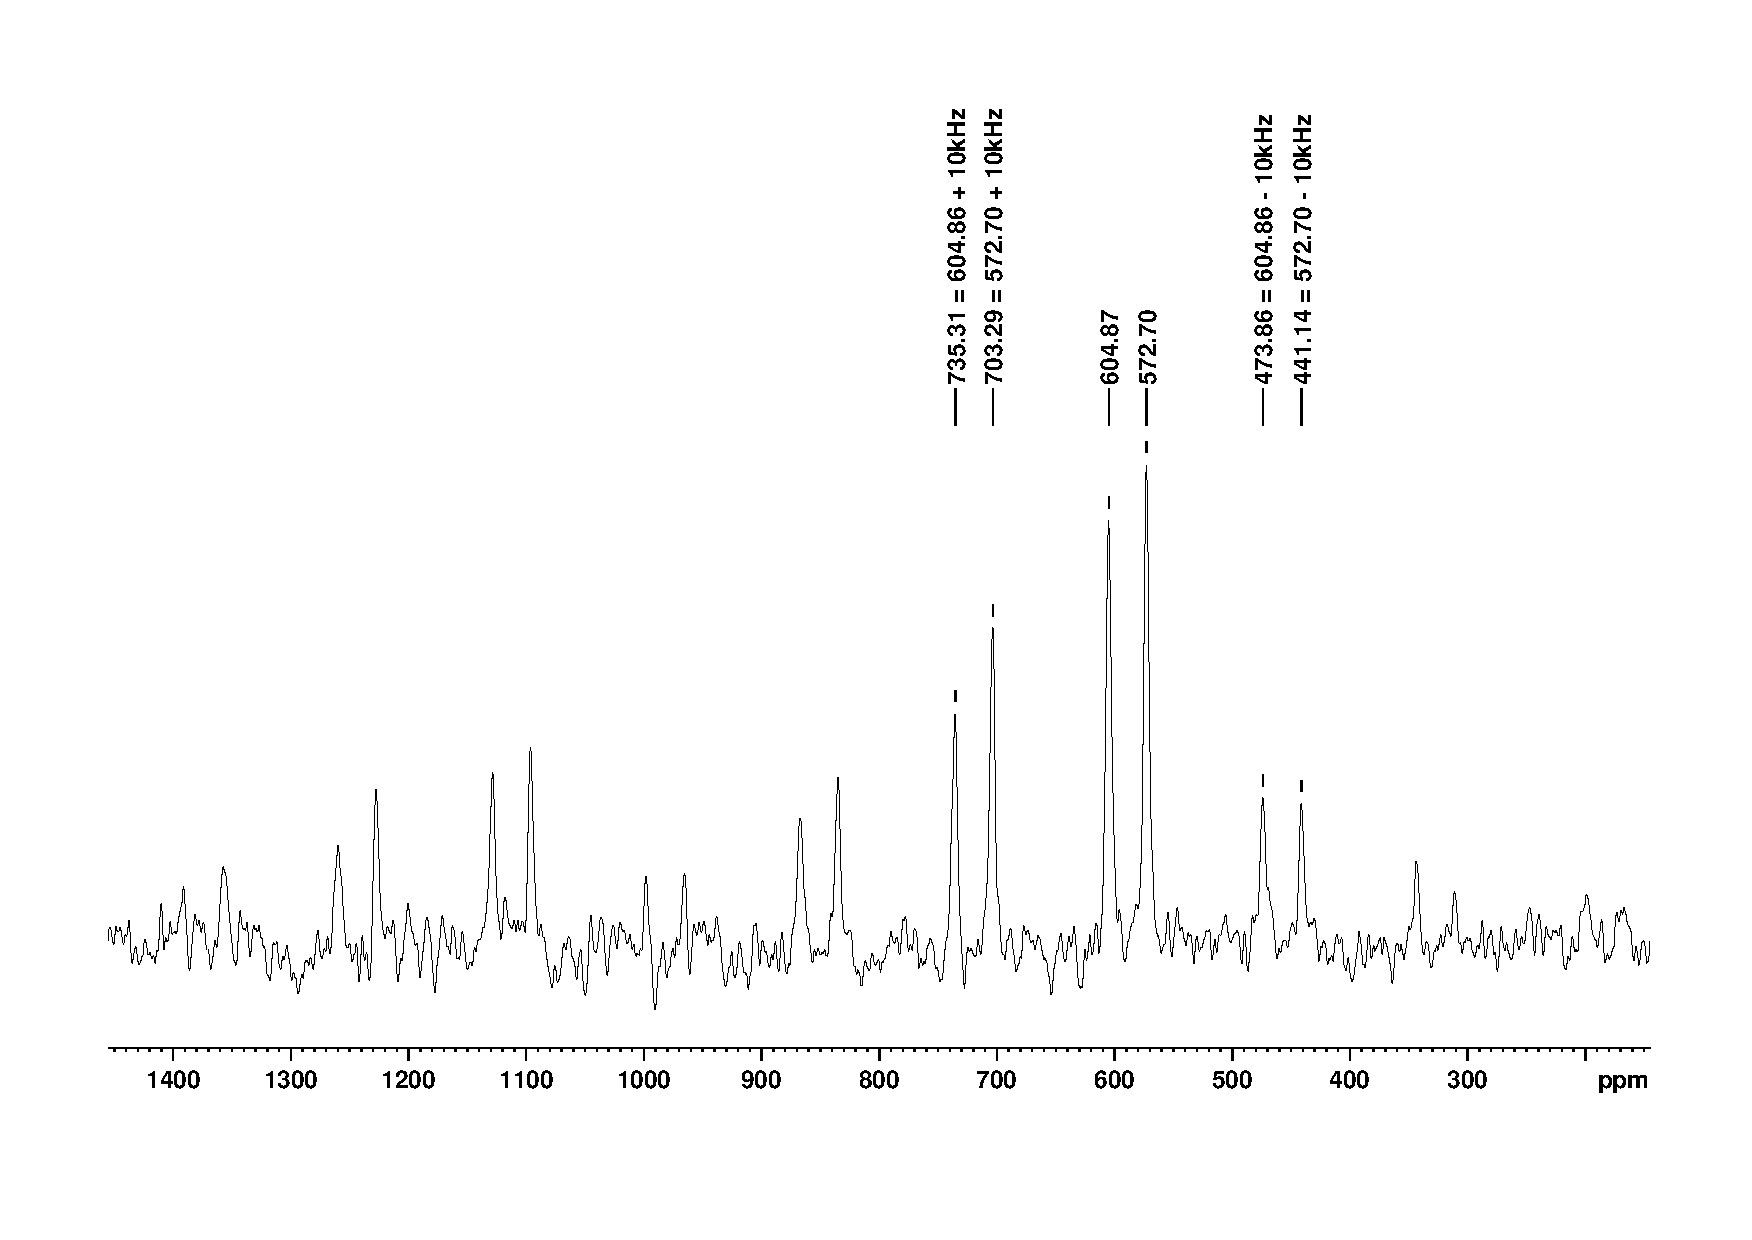
\includegraphics[width=0.7\linewidth]{Figures/ebs-4ome-dmap-cpmas-77se.pdf}
    \caption[Solid state \ce{^{77}Se}-NMR spectrum of \refcmpd{ebs.4ome}$\cdot$DMAP.]{Solid state \ce{^{77}Se}-NMR spectrum of \refcmpd{ebs.4ome}$\cdot$DMAP. The primary resonances are visible at 834.69 and 867.02~ppm. The remaining peaks are spinning sidebands, and are separated from the parent signals by multiples of 10~kHz (the magic angle spinning frequency).}
    \label{fig:cpmas-sol-77se}
\end{figure}

\subsection{Measurement of chemical shift anisotropy}
We acquired solid state spectra of three complexes spanning the range of electron demand, \cmpd{ebs.4ome}$\cdot$DMAP, \cmpd{ebs}$\cdot$DMAP, and \cmpd{ebs.4no2}$\cdot$DMAP.
\footnote{\cmpd{ebs.4ome}$\cdot$DMAP differs from the other structures, in that it crystallises in the space group $P2_1/c$, whereas \cmpd{ebs}$\cdot$DMAP and \cmpd{ebs.4no2}$\cdot$DMAP both crystallise in $P\bar{1}$.
The $2_1$ screw axis in the former crystal is oriented such that it generates a symmetry equivalent molecule which is rotated by an angle of about 45\degree.
This means that the observed chemical shift tensor is the average of these two symmetry related orientations, further complicating the analysis.
Fundamentally this is due to the fact that an ellipsoid does not have twofold rotational symmetry, except about its principal axes.
The triclinic complexes \cmpd{ebs}$\cdot$DMAP and \cmpd{ebs.4no2}$\cdot$DMAP do not suffer from this issue, as the inversion symmetry operation preserves the shape of the tensor.
This can be seen in the latter two principal values of the chemical shift tensor in \cref{tab:77se-ssnmr-ebs-csa}, which have the same value (within experimental error), describing a cigar-shaped tensor.}
The resulting spectra are presented in \cref{fig:77se-ssnmr-ebs}, and the extracted principal values of the chemical shift tensor are presented in \cref{tab:77se-ssnmr-ebs-csa}.

\begin{figure}
  \centering
  \begin{subfigure}{\linewidth}
    \centering
    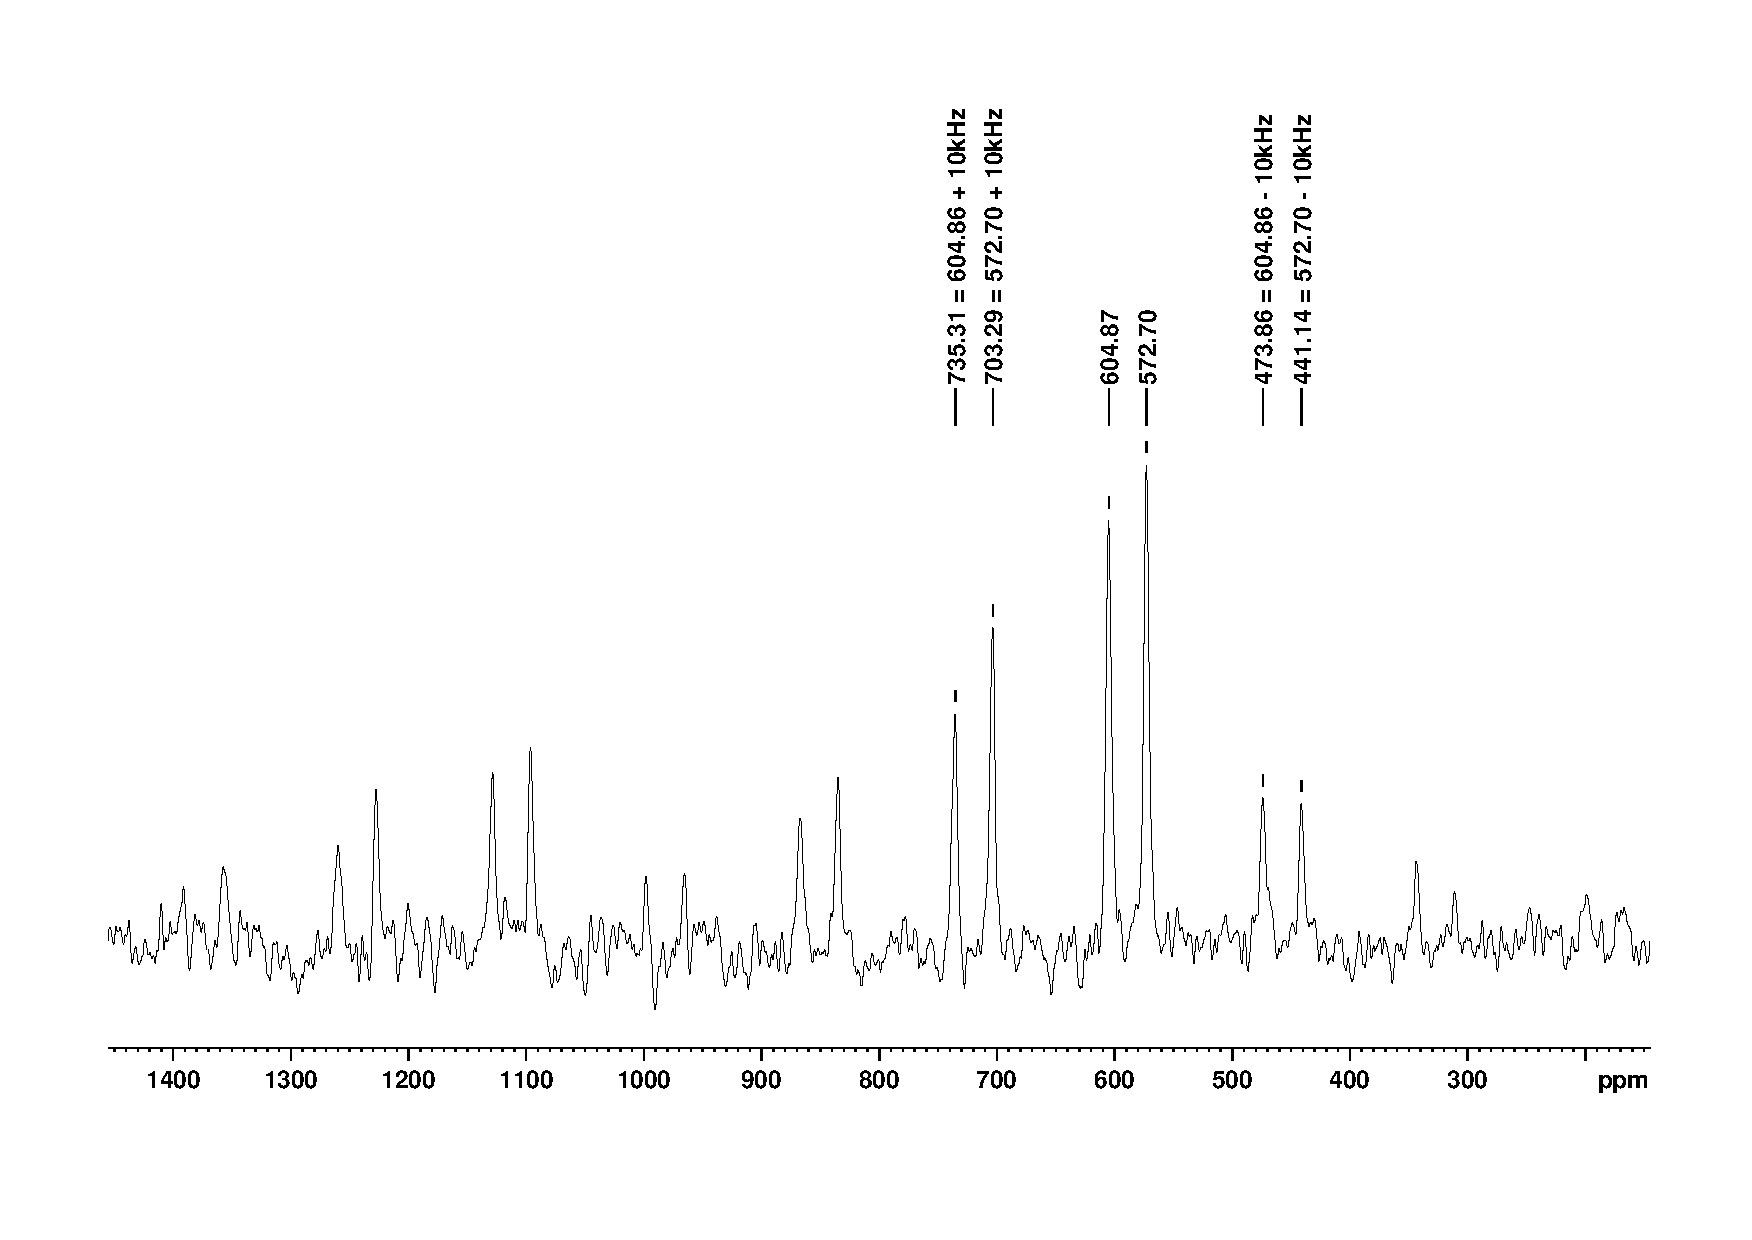
\includegraphics[height=0.28\textheight]{Figures/ebs-4ome-dmap-cpmas-77se.pdf}
    \caption{\ce{^{77}Se} CPMAS NMR spectrum of \refcmpd{ebs.4ome}$\cdot$DMAP.}
  \end{subfigure}
  \begin{subfigure}{\linewidth}
    \centering
    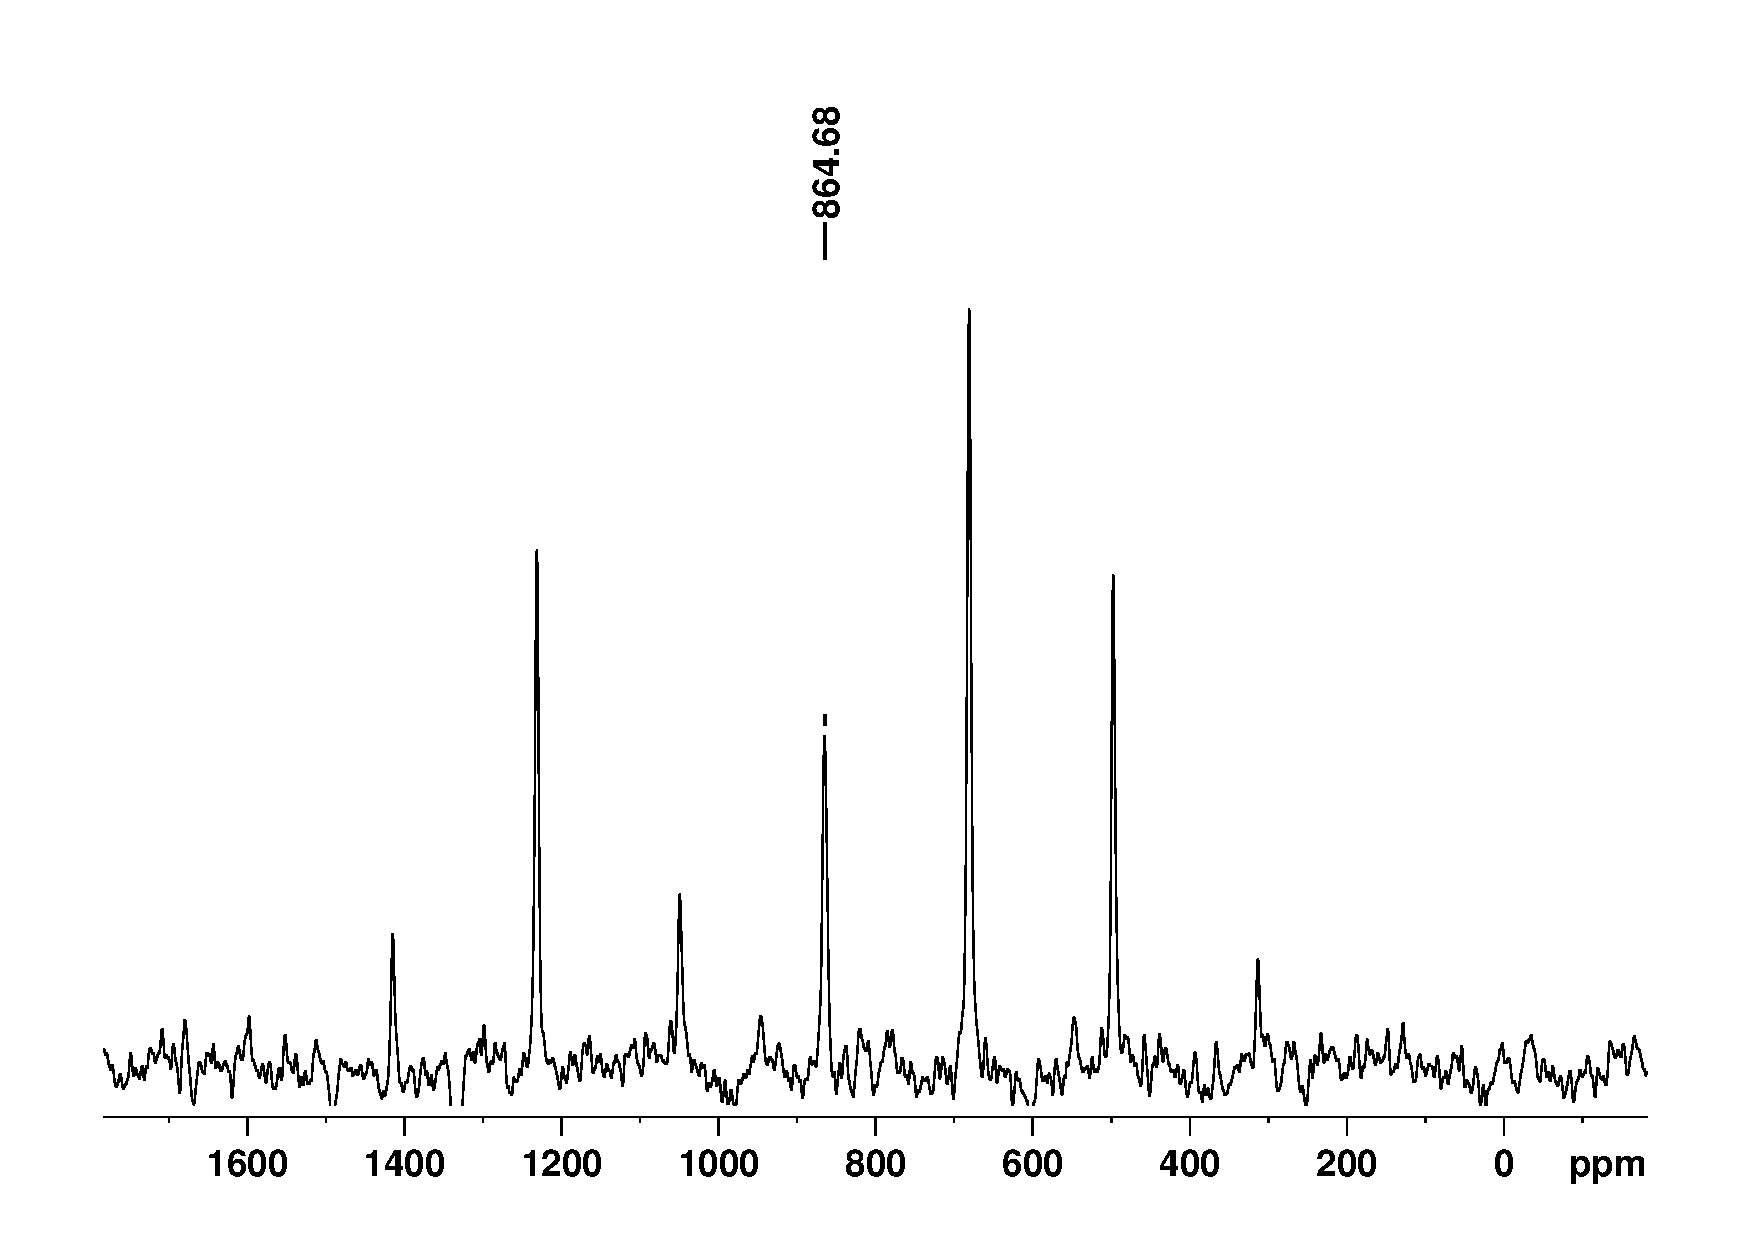
\includegraphics[height=0.28\textheight]{Figures/ebs-ph-dmap-cpmas-77se.pdf}
    \caption{\ce{^{77}Se} CPMAS NMR spectrum of \refcmpd{ebs}$\cdot$DMAP.}
  \end{subfigure}
  \begin{subfigure}{\linewidth}
    \centering
    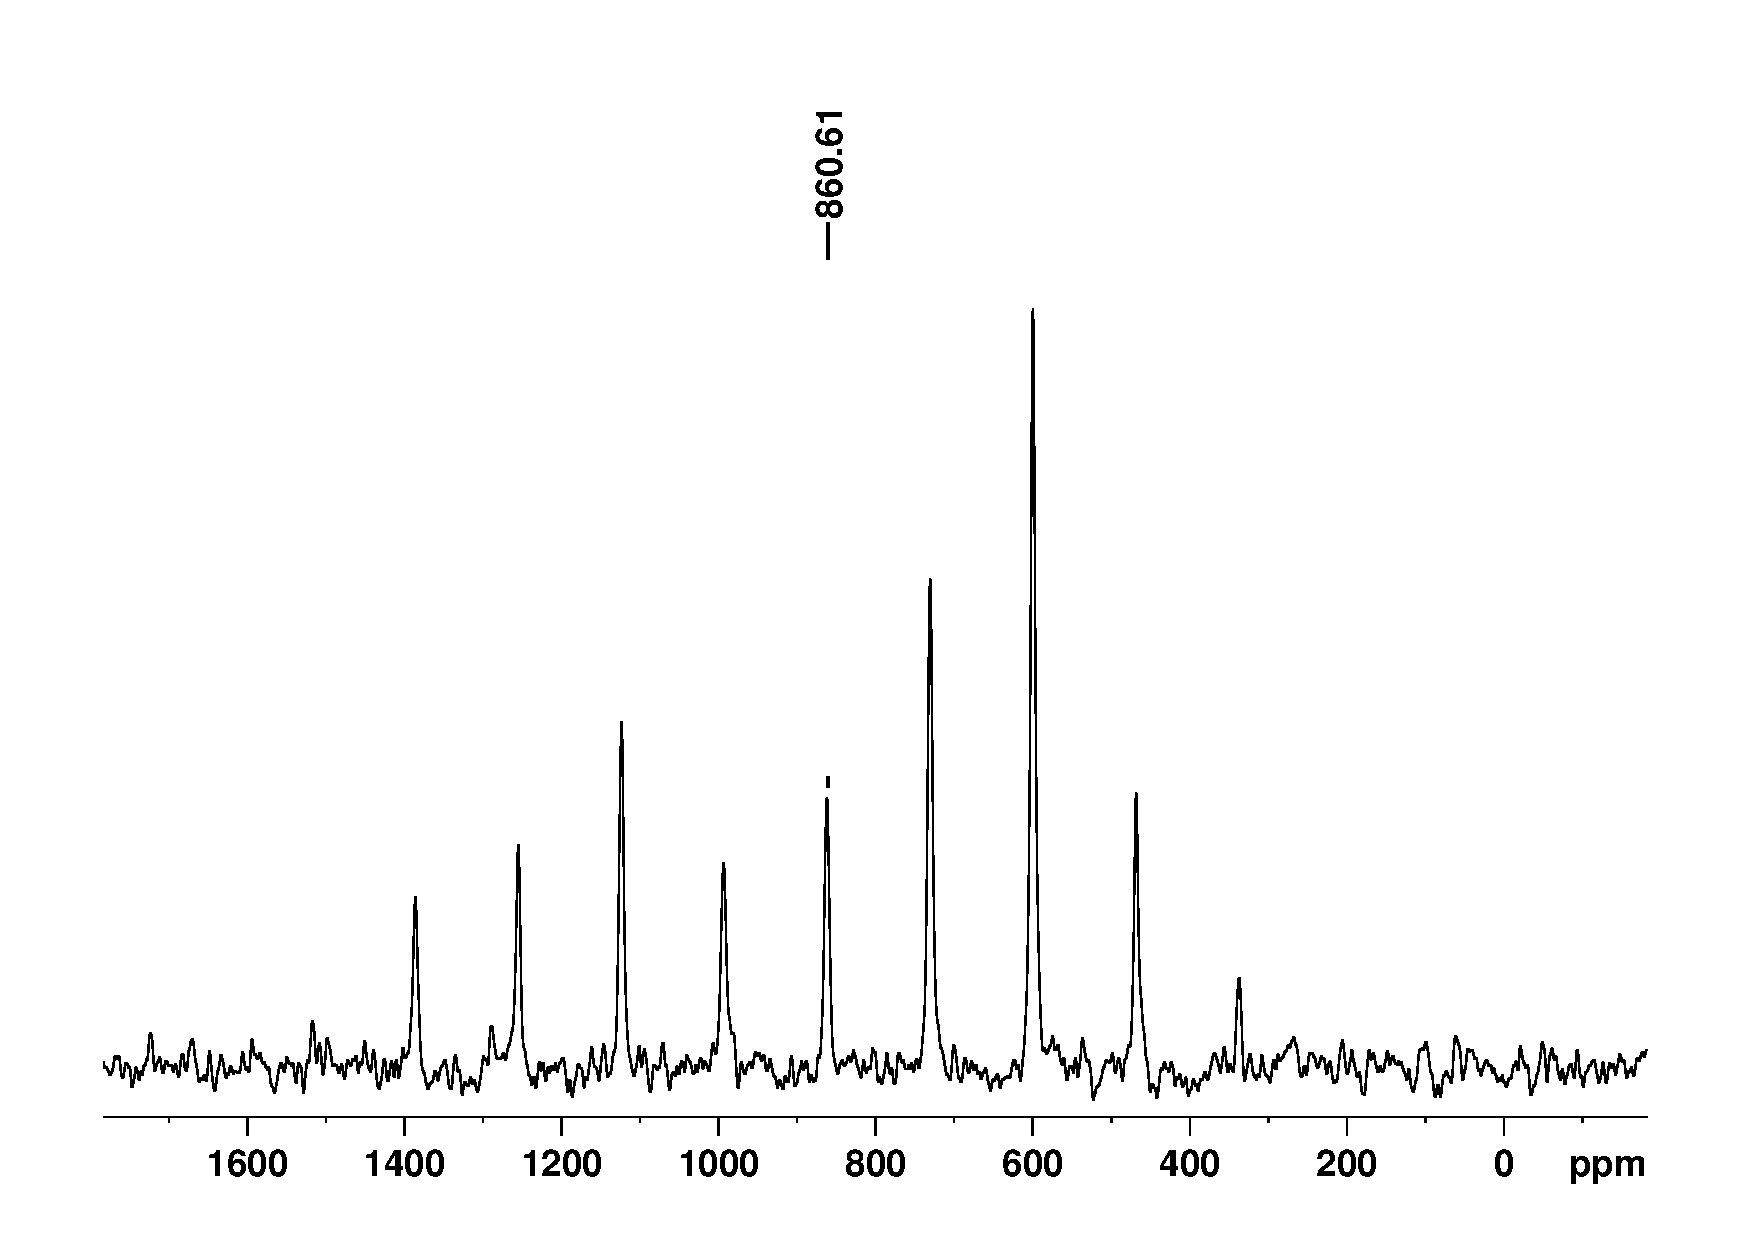
\includegraphics[height=0.28\textheight]{Figures/ebs-4no2-dmap-cpmas-77se.pdf}
    \caption{\ce{^{77}Se} CPMAS NMR spectrum of \refcmpd{ebs.4no2}$\cdot$DMAP.}
  \end{subfigure}
  \caption[\ce{^{77}Se} CPMAS NMR spectra for ebselen derivatives.]{}
  \label{fig:77se-ssnmr-ebs}
\end{figure}

\begin{table}
  \caption{Principal values of the chemical shift tensor extracted from powder spectra in \cref{fig:77se-ssnmr-ebs}.}
  \begin{tabular}{lllll}
    \toprule
    Complex                                    & $\delta_{\textrm{iso}}$ & $\delta_{11}$  & $\delta_{22}$  & $\delta_{33}$   \\\midrule
   \cmpd{ebs.4ome}$\cdot$DMAP\tablefootnote{Site a}   & 835.2                   & 1572.58        & 466.52         & 466.50          \\
   \cmpd{ebs.4ome}$\cdot$DMAP\tablefootnote{Site b}   & 866.9                   & 1628.91        & 485.95         & 485.92          \\
   \cmpd{ebs}$\cdot$DMAP                           & 864.5                   & 1616.74        & 596.21         & 380.64          \\
   \cmpd{ebs.4no2}$\cdot$DMAP                         & 860.8                   & 1596.92        & 547.82         & 437.66          \\\bottomrule
  \end{tabular}
  \label{tab:77se-ssnmr-ebs-csa}
\end{table}


\subsection{Calculation of chemical shift anisotropy}
In order to verify our results, we also \emph{calculated} the chemical shielding tensors in order to compare the principal values, and also determine the likely orientation of the tensors with respect to the rest of the molecule (\cref{fig:77se-tensor-ebs-dmap}).
These calculations were conducted at the $\omega$B97X-D/def2TZVP level, using the GIAO method of calculating shielding tensors.\autocite{Schreckenbach1995CalculationTheory,Schreckenbach1996TheApproximation}
In order to convert these chemical shielding tensors $\sigma$ into chemical shifts $\delta$, we must reference them to a standard $\sigma_{\textrm{ref}}$.
\begin{equation}
  \delta = \sigma_{\textrm{ref}} - \sigma_{\textrm{sample}}
  \label{eqn:shieldingtoshift}
\end{equation}
Convention dictates that for \ce{^{77}Se}, dimethylselenide is assigned a chemical shift of 0~ppm.
The structure of dimethylselenide was therefore optimised and shielding tensors calculated at the same level.

The tensors (in the computation reference frame) were found to be
\begin{align*}
  \sigma_{\textrm{\ce{Me2Se}}} = &\begin{bmatrix} 2276.3834 & -0.0073 & -0.0175 \\ -0.0159 & 1579.1094 & 0.0349 \\ -0.0622 & -0.0041 & 1583.4669 \end{bmatrix}\\
  \sigma_{\textrm{\cmpd{ebs}}} = &\begin{bmatrix} 1086.4346 & 929.1822 & 929.1822 \\ 862.9168 & 514.6826 & -87.328 \\ 105.4202 & -92.4104 & 1101.0194 \end{bmatrix}\\
  \sigma_{\textrm{\cmpd{ebs.4ome}}\cdot\textrm{DMAP}} = &\begin{bmatrix} 1686.2267 & 105.2547 & -3.2274 \\ 31.1129 & 187.9487 & 48.4737 \\ -19.1247 & 50.3984 & 1081.5651 \end{bmatrix}\\
  \sigma_{\textrm{\cmpd{ebs}}\cdot\textrm{DMAP}} = &\begin{bmatrix} 1595.7999 & 367.4957 & 6.7322 \\ 322.6389 & 291.3611 & 10.8588 \\ -19.9165 & -35.8017 & 1069.2648 \end{bmatrix}\\
  \sigma_{\textrm{\cmpd{ebs.4no2}}\cdot\textrm{DMAP}} = &\begin{bmatrix} 1671.4068 & -76.2797 & 20.6203 \\ -100.0242 & 221.8577 & -17.9295 \\ -44.1025 & -120.0346 & 1055.0806 \end{bmatrix}\\
  \sigma_{\textrm{\cmpd{ebs}}\cdot\textrm{DMF}} = &\begin{bmatrix} 1642.3856 & -138.5717 & -175.547 \\ -111.063 & 175.617 & -253.364 \\ -215.991 & -275.178 & 1028.493 \end{bmatrix}
\end{align*}

affording reference frame independent principal values in \cref{tab:77se-calc-ebs-shielding-csa}.

\begin{table}
  \caption{Principal values of the chemical shielding tensor calculated from optimised structures.}
  \begin{tabular}{lllll}
    \toprule
    Complex                                           & $\sigma_{\textrm{iso}}$ & $\sigma_{11}$  & $\sigma_{22}$  & $\sigma_{33}$   \\\midrule
    \ce{Me2Se}                                        & 1812.9866           & 1579.1093& 1583.4670 & 2276.3834  \\
    \cmpd{ebs}                                     & 900.7122            & -156.9566& 1114.4138 & 1744.6794  \\
    \cmpd{ebs.4ome}$\cdot$DMAP                        & 985.2468            & 182.0846 & 1084.2014 & 1689.4545  \\
    \cmpd{ebs}$\cdot$DMAP                          & 985.4753            & 205.5761 & 1069.2485 & 1681.6013  \\
    \cmpd{ebs.4no2}$\cdot$DMAP                        & 982.7817            & 210.7844 & 1060.7206 & 1676.8400  \\
    \cmpd{ebs}$\cdot$DMF                           & 948.8319            & 80.7668  & 1064.7403 & 1700.9887  \\
    \bottomrule
  \end{tabular}
  \label{tab:77se-calc-ebs-shielding-csa}
\end{table}

These were converted to chemical shifts using \cref{eqn:shieldingtoshift}, which are presented in \cref{tab:77se-calc-ebs-shift-csa}.

\begin{table}
  \caption{Principal values of the chemical shift tensor calculated from optimised structures.}
  \begin{tabular}{lllll}
    \toprule
    Complex                                           & $\delta_{\textrm{iso}}$ & $\delta_{11}$  & $\delta_{22}$  & $\delta_{33}$   \\\midrule
    \cmpd{ebs}                                     & 912.2744            & 1969.9432& 698.5728  & 68.3072    \\
    \cmpd{ebs.4ome}$\cdot$DMAP                        & 827.7398            & 1630.9020& 728.7852  & 123.5321   \\
    \cmpd{ebs}$\cdot$DMAP                          & 827.5113            & 1607.4105& 743.7381  & 131.3853   \\
    \cmpd{ebs.4no2}$\cdot$DMAP                        & 830.2049            & 1602.2022& 752.2660  & 136.1466   \\
    \cmpd{ebs}$\cdot$DMF                           & 864.1547            & 1732.2198& 748.2463  & 111.9979   \\ \bottomrule
  \end{tabular}
  \label{tab:77se-calc-ebs-shift-csa}
\end{table}

These values are encouragingly close to those derived from the fitting of the experimental MAS line shape, with the exception of \cmpd{ebs.4ome}$\cdot$DMAP, for reasons explained above.

Plotting the resulting tensors as ellipsoids reveals aspects of the electron density and hence shielding around the selenium (\cref{fig:77se-tensor-ebs-dmap}).
A major contributor to the tensor is of course the aromatic ring current, which leads to deshielding perpendicular to the plane of the ring.
There is also a ring current in the pyridine ring, which deshields the selenium roughly in the direction of the \ce{Se-C} bond (perpendicular to the plane of the pyridine ring).
This accounts for the large $\delta_{11}$ and $\delta_{22}$ components of the chemical shift.
The remainder is presumably due to diamagnetic shielding from the electron density.
In this we are able to see deformation of the electron cloud due to the lone pairs and the Ch-bond.
The  $\delta_{33}$ component is substantially smaller than $\delta_{11}$ and $\delta_{22}$, and is aligned with the Ch-bond, reflecting a very strong shielding in this direction.
This clearly shows the contribution of the lone pair of the pyridyl nitrogen to the electron density around the selenium, and hence the strength of the Ch-bond.

\begin{figure}
  \centering
  \begin{subfigure}{0.3\linewidth}
    \centering
    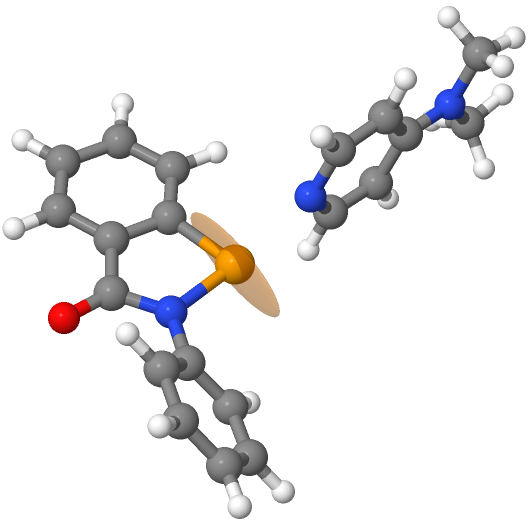
\includegraphics[height=3.5cm]{Figures/77se-tensor-ebs-dmap.png}
    \caption{Calculated chemical shift tensor for \refcmpd{ebs}$\cdot$DMAP.}
    \label{fig:77se-tensor-ebs-dmap}
  \end{subfigure}
  \begin{subfigure}{0.3\linewidth}
    \centering
    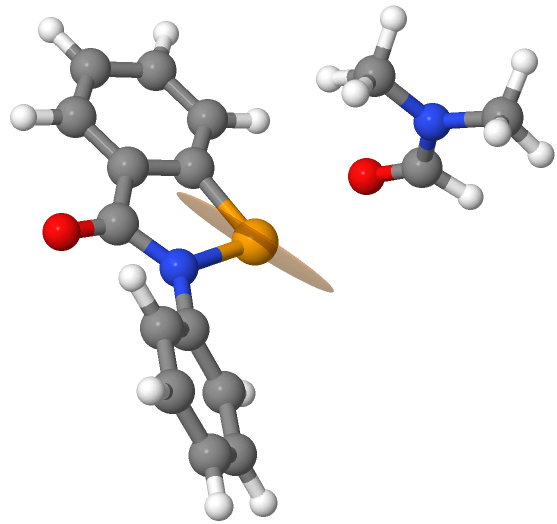
\includegraphics[height=3.5cm]{Figures/77se-tensor-ebs-dmf.png}
    \caption{Calculated chemical shift tensor for \refcmpd{ebs}$\cdot$DMF.}
    \label{fig:77se-tensor-ebs-dmf}
  \end{subfigure}
  \begin{subfigure}{0.3\linewidth}
    \centering
    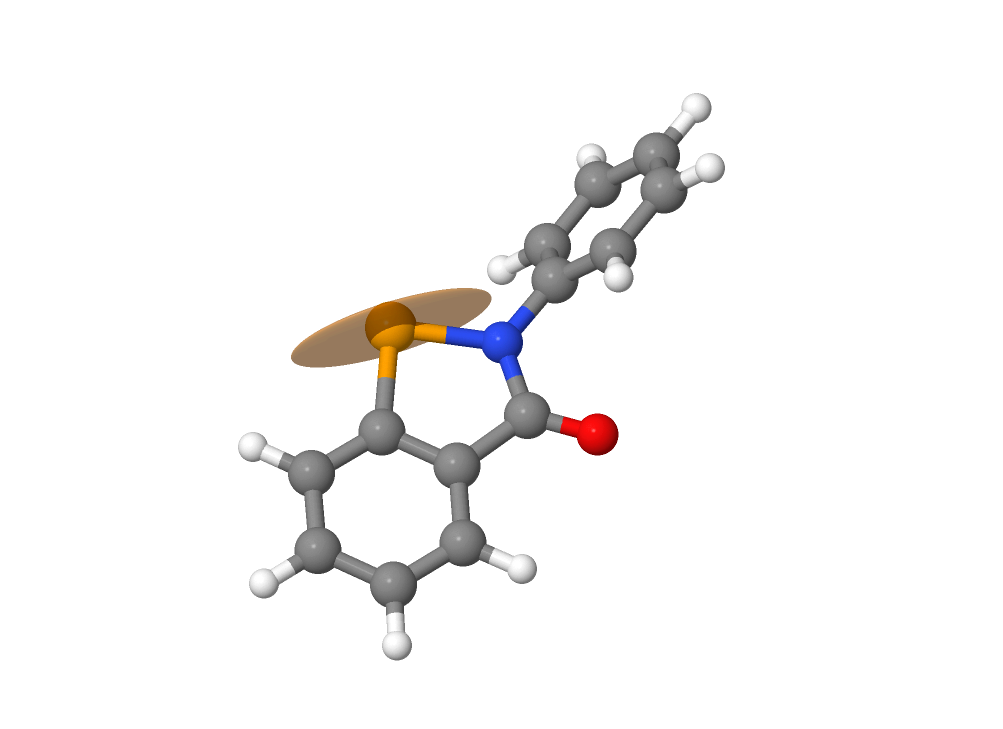
\includegraphics[height=3.5cm]{Figures/77se-tensor-ebs.png}
    \caption{Calculated chemical shift tensor for \refcmpd{ebs}.}
    \label{fig:77se-tensor-ebs}
  \end{subfigure}
  \caption[Calculated chemical shift tensors for ebselen derivatives.]{}
\end{figure}

This can be contrasted to the chemical shift of the non-complexed selenium (\cref{fig:77se-tensor-ebs}).
In the absence of the lone pair of the pyridyl nitrogen, the $\sigma$-hole strongly deshields the selenium, therefore the large $\delta_{11}$ component is roughly aligned with it.
There is also no deshielding ring current from the pyridine, so the $\delta_{33}$ (which is aligned with the \ce{Se-C} bond) is very small.
The $\delta_{22}$ component perpendicular to the plane of the benzisoselenazolinone ring is roughly the same, as there is no significant change in either electron density or ring currents in this direction.

To demonstrate that the $\delta_{11}$ component in the \cmpd{ebs}$\cdot$DMAP complex is not entirely due to the pyridine ring current, a \cmpd{ebs}$\cdot$DMF complex was optimised and the chemical shift tensor calculated.
This is shown in \cref{fig:77se-tensor-ebs-dmf}.
The largest component of the tensor is still approximately aligned with the \ce{Se-C} bond, even in the absence of the aromatic base.

These results must be taken with a grain of salt, as the chemical shifts are calculated in the gas phase (i.e. in the absence of crystal packing).
This is particularly important for the chemical shift of the non-complexed heterocycle, as such a ``free'' $\sigma$-hole would not be observed in any condensed phase (it is always filled by solvent in solution, or the carbonyl of an adjacent molecule in the solid).
Nonetheless we may draw comparisons with this caveat in mind.

\subsubsection{Measurement of CSA in a single crystal}
The calculated chemical shift tensors were useful in the absence of experimental data, and the fact that the principal values of the tensors matched the powder data so well was encouraging.
However, we wished to verify the orientation of the tensor by an experimental method.

We were fortunate to obtain a single crystal of \cmpd{ebs}$\cdot$DMAP of sufficient size (approx $10\times3\times1$~mm, \cref{fig:ebs-ph-dmap-picture}) for a single crystal SS-NMR experiment, allowing us to measure the orientation of the tensor in that crystal for comparison with our computational results.\footnote{Unfortunately no other derivatives formed crystals of sufficient size or morphology for the SS-NMR experiment.}

\begin{figure}
  \centering
  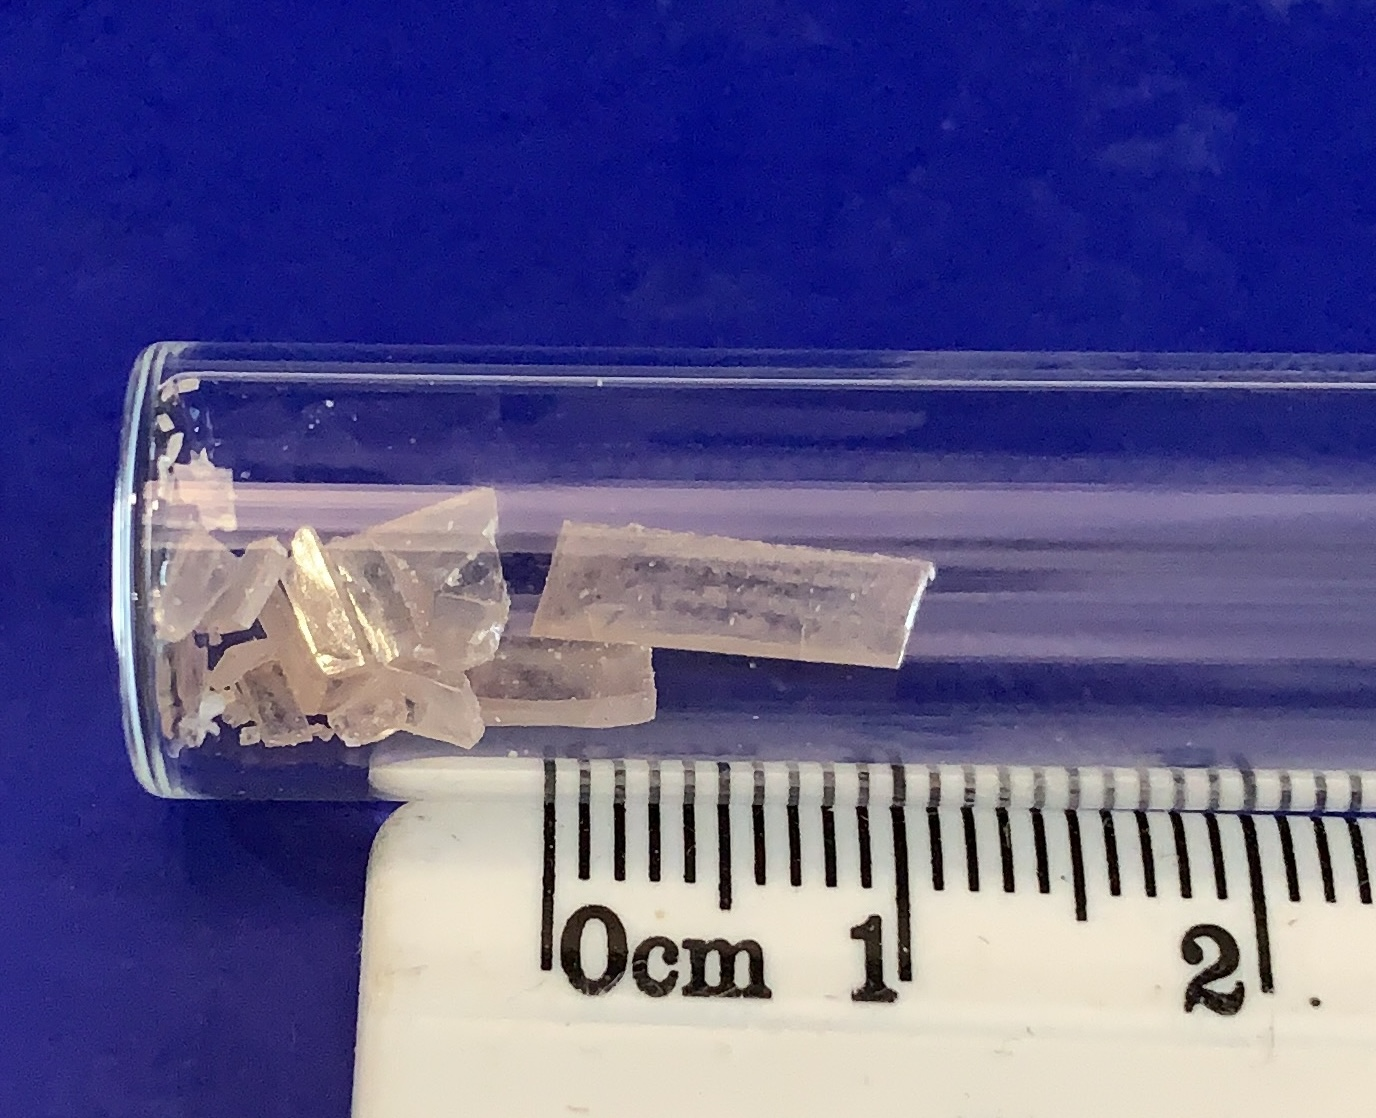
\includegraphics[width=0.4\linewidth]{Figures/ebs-ph-dmap-picture.jpg}
  \caption{Single crystal of \cmpd{ebs}$\cdot$DMAP used for SS-NMR.}
  \label{fig:ebs-ph-dmap-picture}
\end{figure}

In order to do this, the faces of the crystal had to be indexed to the internal structure, which was done by x-ray diffraction.
As the crystal was far too big to mount on the diffractometer, two faces were marked with different coloured pens to preserve the relation to the large crystal, then a small fragment was removed from the crystal.
This was mounted, and a short data collection afforded an indexable pattern.
The resulting planes are shown in \cref{fig:ebs-ph-dmap-index}.

\begin{figure}
  \centering
  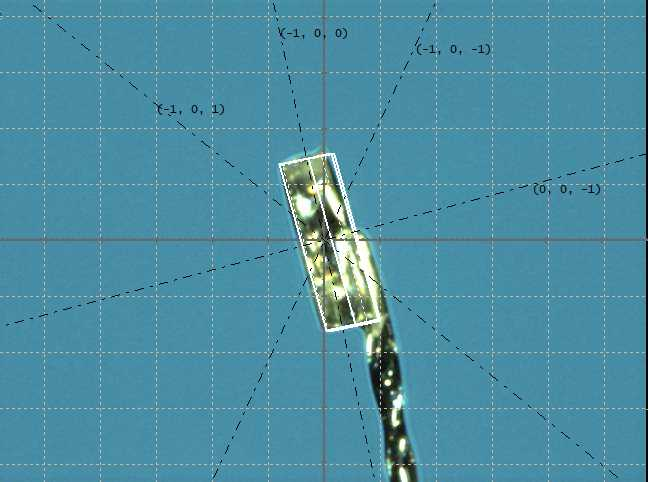
\includegraphics[width=0.48\linewidth]{Figures/xtal-b.jpg}
  \includegraphics[width=0.48\linewidth]{Figures/xtal-c.jpg}
  \caption{Indexed faces of \cmpd{ebs}$\cdot$DMAP.}
  \label{fig:ebs-ph-dmap-index}
\end{figure}

A number of these large crystals were visually indexed based on their morphology, and packed in a rectangular sample holder.
Spectra were acquired on a 600~MHz instrument using a Hahn echo pulse sequence.
This was necessary to preseve the extremely weak signal by isolating it from the excitation pulse in the time domain.
The spectra were referenced to a saturated solution of diphenyldiselenide in \ce{CDCl3} at 463~ppm, which was contained in a zirconia MAS rotor inside the sample holder.\autocite{Duddeck1995}

The crystal orientation with respect to the magnetic field is depicted in \cref{fig:ebs-ph-dmap-magfield-index}, and the resulting spectrum is shown in \cref{fig:ebs-dmap-hahnecho-77se}.
The selenium nucleus in this orientation resonates at 448~ppm.

\begin{figure}
  \centering
  \includegraphics[width=0.3\linewidth]{Figures/ebs-ph-dmap-magfield-index.pdf}
  \caption[Orientation of the magnetic field with respect to the crystal.]{Orientation of the magnetic field with respect to the crystal. $B_{0}$ is aligned with the $[0 0 1]$ crystal direction. Note that the crystal is actually triclinic ($\alpha\neq\beta\neq\gamma\neq 90$\degree), but the $\alpha$ and $\beta$ angles are sufficiently close to 90\degree\ that we can treat the (001) plane as approximately perpendicular to the [001] axis.}
  \label{fig:ebs-ph-dmap-magfield-index}
\end{figure}

\begin{figure}
  \centering
  \includegraphics[width=0.8\linewidth]{Figures/ebs-dmap-hahnecho-77se.pdf}
  \caption{\ce{^{77}Se} NMR spectrum of a single crystal of \refcmpd{ebs}$\cdot$DMAP in the orientation depicted in \cref{fig:ebs-ph-dmap-magfield-index}.}
  \label{fig:ebs-dmap-hahnecho-77se}
\end{figure}

The sample holder was then re-packed with the crystals now rotated 90\degree\ to their original orientaton, and a spectrum was again acquired.
This is shown in \cref{fig:ebs-dmap-hahnecho-77se2,fig:ebs-ph-dmap-magfield-index2}, where the selenium now resonates at 567~ppm

\begin{figure}
  \centering
  \includegraphics[width=0.3\linewidth]{Figures/ebs-ph-dmap-magfield-index2.pdf}
  \caption[Orientation of the magnetic field with respect to the crystal.]{Orientation of the magnetic field with respect to the crystal. $B_{0}$ is aligned with the $[0 1 0]$ crystal direction}
  \label{fig:ebs-ph-dmap-magfield-index2}
\end{figure}

\begin{figure}
  \centering
  \includegraphics[width=0.8\linewidth]{Figures/ebs-dmap-hahnecho-77se2.pdf}
  \caption[\ce{^{77}Se} NMR spectrum of a single crystal of \refcmpd{ebs}$\cdot$DMAP in the orientation depicted in \cref{fig:ebs-ph-dmap-magfield-index2}.]{\ce{^{77}Se} NMR spectrum of a single crystal of \refcmpd{ebs}$\cdot$DMAP in the orientation depicted in \cref{fig:ebs-ph-dmap-magfield-index2}. The smaller satellite signals are due to slightly misaligned crystals in the sample holder. This also explains the poorer signal to noise ratio of the main peak.}
  \label{fig:ebs-dmap-hahnecho-77se2}
\end{figure}

In order to orient the tensor in the laboratory reference frame, we must determine the declination and azimuth angles $\theta$ and $\phi$.
This is done by writing an expression which relates these angles, the principal values (determined from the powder experiment), and the observed chemical shift.
The rotation of the tensor into the lab reference frame is modelled by a simple rotation matrix of the two polar angles:
\begin{equation}
  \mathbf{Q} = \begin{bmatrix} \cos\theta & 0 & \sin\theta \\ \sin\theta\sin\phi  & \cos\phi & -\cos\theta\sin\phi \\ -\sin\theta\cos\phi & \sin\phi & \cos\theta\cos\phi \end{bmatrix}
\end{equation}
The 90\degree\ rotation about the \textit{a} axis is modelled by a similar rotation matrix which, for generality, is derived from the Rodrigues rotation formula describing a rotation of angle $\psi$ about a unit vector $\hat{\omega} = \left( \omega_{x}, \omega_{y}, \omega_{z} \right)$:
\begin{equation}
  \mathbf{R}_{\hat{\omega}}(\psi) = \mathbf{I} + \tilde{\omega}\sin\psi + \tilde{\omega}^{2}(1-\cos\psi)
\end{equation}
where $\tilde{\omega}$ is the antisymmetric matrix:
\begin{equation}
  \tilde{\omega} = \begin{bmatrix} 0 & -\omega_{z} & \omega_{y} \\ \omega_{z} & 0 & -\omega_{x} \\ -\omega_{y} & \omega_{x} & 0 \end{bmatrix}
\end{equation}
and $\mathbf{I}$ denotes the $3\times 3$ identity matrix.
This notation is particularly convenient for crystallography, as the unit vector for a rotation is easily generated from the Miller indices, which generally correspond to a macroscopic face of a crystal.
In this case the rotation axis was simply $\hat{\omega} = (1,0,0)$ i.e. the \textit{a} axis.

Sequentially applying these two rotations allows us to represent the tensor in any orientation.
The projection of the tensor onto the Z axis (the magnetic field $B_{0}$), which coresponds to the observed chemical shift in any given orientation, is given by the $\delta_{ZZ}$ component of the tensor.
We therefore simply optimise the function
\begin{equation}
  \delta = \mathbf{R} \mathbf{Q} \begin{bmatrix} 1616.74 & 0 & 0 \\ 0 & 596.21 & 0 \\ 0 & 0 & 380.64 \end{bmatrix} \mathbf{Q}^{-1} \mathbf{R}^{-1}
\end{equation}
to reproduce the observed $\delta_{Z,Z}$ components for $\psi = 0$\degree\ and $\psi = 90$\degree.
The polar angles thus calculated are equal to $\theta = 79.9$\degree\ and $\phi = 23.8$\degree.

We can calculate the chemical shift tensor using the diagonal components from the powder experiment and the rotation matrix from the polar angles which affords
\begin{equation}
  \delta = \begin{bmatrix} 1578.72 & -86.12 & 195.26 \\ -86.12 & 567.29 & 65.55 \\ 195.26 & 65.55 & 447.56 \end{bmatrix}
\end{equation}

This can be plotted within the unit cell of the crystal, where we observe an excellent qualitative agreement with the calculated tensor (\cref{fig:expt-tensor-ebs-dmap}).
The most deshielded axis is aligned with the \ce{Se-C} bond, and the most shielded axis is aligned with the Ch-bond, as in the calculated tensor.
This verifies that the tensor is oriented correctly in the crystal, and that the observed shielding is due to the approach of the lone pair into the $\sigma$-hole.

\begin{figure}
  \centering
  \includegraphics[width=0.7\linewidth]{Figures/expt-tensor-ebs-dmap.pdf}
  \caption[Experimentally determined chemical shift tensor for \refcmpd{ebs}$\cdot$DMAP.]{Experimentally determined chemical shift tensor for \refcmpd{ebs}$\cdot$DMAP. Compare with the calculated tensor in \cref{fig:77se-tensor-ebs-dmap}.}
  \label{fig:expt-tensor-ebs-dmap}
\end{figure}

To briefly summarise, Ch-bonding induces enormous chemical shift anisotropy at the selenium, which is highly sensitive to the approach of the Lewis base and can be measured using both powder and single crystal SS-NMR.
While the technique is perhaps not as sensitive as diffraction based methods, the great advantage lies in the fact that SS-NMR does not require crystallinity, even at the nano scale.
This means that amorphous species such as polymers may be studies, as long as they contain an NMR active nucleus.

\subsection{Solution-phase studies}
While the above crystallographic analysis gives a useful qualitative understanding of the strength of the Ch-bond, we sought an experimental method that could accurately determine bond energies, so that we could easily compare our Ch-bonded complexes with those dominated by other interactions.

\subsubsection{NMR titration experiments}
NMR titrations are a useful tool for the determination of binding affinities in supra\-molecular and host-guest chemistry.\autocite{???}
\ce{^{1}H} and \ce{^{19}F} NMR have both been used to study halogen bonded systems, however we decided to take advantage of the unique NMR characteristics of the \ce{^{77}Se} nucleus to probe the Ch-bond in our systems for the following reasons:

\begin{itemize}
    \item the nucleus has an extremely wide chemical shift range (-1000--2000~ppm),
    \item the chemical shift is very sensitive to the electronic environment around the selenium,
    \item the selenium is at the heart of the interaction, so any electronic changes should manifest clearly,
    \item the spectrum (for our compounds) is extremely simple, featuring only one singlet,
    \item the experiment is moderately sensitive (slightly more sensitive than \ce{^{13}C}).
\end{itemize}

We devised a titration experiment, where a solution of a Lewis base is gradually added to a solution of the Ch-bond donor, and the chemical shift of the selenium is measured at the various concentrations of base.
As the concentration of base increases, a greater proportion of the selenium species will be in a Ch-bonded environment, with an associated increase in electron density at the selenium due to the coordinated base.
This will lead to an upfield shift of the selenium resonance.

It is important to note that even in the absence of a Lewis base, the organoselenium species will still likely feature a Ch-bond to the carbonyl oxygen of another molecule.
This is substantially weaker than a \ce{Se\dots N} interaction, but non-negligible.
We must therefore view these as \emph{competition} experiments, rather than an absolute measure of binding energy.

For single site binding (a valid approximation for these systems, as the single $\sigma$-hole is likely to out-compete all other interactions), the dissociation constant can be expressed as

\begin{equation}
    \label{eqn:equilibrium}
    \mathrm{K_d} = \frac{[\mathrm{ebs}][\mathrm{base}]}{[\mathrm{ebs\cdot base}]}
\end{equation}

If the Ch-bond formation/breaking is slow on the NMR timescale, two distinct resonances will be observed that correspond to the ``free'' (Ch-bonded to a carbonyl oxygen) and ``bound'' (Ch-bonded to the Lewis base) selenium species, and their relative concentrations can be determined by integration of the signals.
As it happens, this is not the case, and the process is fast relative to the NMR timescale.
The observed chemical shift is therefore the mole fraction ($f_\mathrm{ebs} = [\mathrm{ebs}]/[\mathrm{ebs}]_0$ and $f_\mathrm{ebs\cdot base} = [\mathrm{ebs\cdot base}]/[\mathrm{ebs}]_0$) weighted average of the chemical shifts of the two species:
\begin{equation}
    \delta_{\mathrm{observed}} = \delta_{\mathrm{ebs}} f_\mathrm{ebs} + \delta_{\mathrm{ebs\cdot base}} f_{\mathrm{ebs\cdot base}}
\end{equation}

If we consider only the \emph{change} in chemical shift from the free species, this becomes simply:
\begin{align}
    \Delta(\delta_{\mathrm{observed}}) & = \Delta(\delta_{\mathrm{ebs\cdot base}}) f_{\mathrm{ebs\cdot base}} \\
    & = \Delta(\delta_{\mathrm{ebs\cdot base}}) \left(\frac{[\mathrm{ebs\cdot base}]}{[\mathrm{ebs}]_0}\right)
\end{align}

From here we can rearrange the equilibrium expression (\cref{eqn:equilibrium}) and mass balance equation ($[\mathrm{ebs}]_0 = [\mathrm{ebs}] + [\mathrm{ebs\cdot base}]$), and substitute them in to arrive at the generic binding isotherm equation:
\begin{equation}
    \Delta(\delta) = \frac{\Delta(\delta_{\mathrm{ebs\cdot base}})  \times [\mathrm{base}]}{\mathrm{K_{d}} + [\mathrm{base}]}
\end{equation}

This assumes that there is insignificant depletion of the base concentration due to complexation.\autocite{Thordarson2011}
Such an assumption may not be entirely valid for this situation, which may explain the imperfect fitting.
However, the analysis is considerably simplified, and adequate standard deviations are obtained using this method.

The resulting K\textsubscript{d} values can be converted to free energies:
\begin{equation}
    \Delta G = -RT \ln{\mathrm{K_d}}
\end{equation}

A saturated solution of the organoselenium derivative in chloroform was used, due to the high solubility (to reduce acquisition time) and non-coordinating nature (to minimise Ch-bonding to the solvent).
This was spiked with a small amount of deuterochloroform for the lock signal.
Spectra were acquired on a 500~MHz instrument, using a 60\degree~pulse and 1~s relaxation delay, until an unambiguous \ce{^{77}Se} resonance was observed.
The resulting chemical shifts were then tabulated and plotted against the concentration of the Lewis base.
These are shown in \cref{fig:nmr-titrations}.

\begin{figure}
  \centering
  \begin{subfigure}{0.45\linewidth}
    \includegraphics[width=\linewidth]{Figures/nmr-titration/bn-ebs-dmap.eps}
    \caption{\refcmpd{ebs.bn}$\cdot$DMAP}
  \end{subfigure}
  \begin{subfigure}{0.45\linewidth}
    \includegraphics[width=\linewidth]{Figures/nmr-titration/4oet-ebs-dmap.eps}
    \caption{\refcmpd{ebs.4oet}$\cdot$DMAP}
  \end{subfigure}
  \begin{subfigure}{0.45\linewidth}
    \includegraphics[width=\linewidth]{Figures/nmr-titration/ebs-dmap.eps}
    \caption{\refcmpd{ebs}$\cdot$DMAP}
  \end{subfigure}
  \begin{subfigure}{0.45\linewidth}
    \includegraphics[width=\linewidth]{Figures/nmr-titration/4br-ebs-dmap.eps}
    \caption{\refcmpd{ebs.4br}$\cdot$DMAP}
  \end{subfigure}
  \begin{subfigure}{0.45\linewidth}
    \includegraphics[width=\linewidth]{Figures/nmr-titration/4cn-ebs-dmap.eps}
    \caption{\refcmpd{ebs.4cn}$\cdot$DMAP}
  \end{subfigure}
  \caption[NMR titration binding isotherms.]{Binding isotherms for ebselen derivatives \refcmpd{ebs.bn,ebs.4oet,ebs,ebs.4br,ebs.4cn} with DMAP. Scatchard plots are inset.}
  \label{fig:nmr-titrations}
\end{figure}

Non-linear regression analysis was performed with the \texttt{nls} function in the R software package using the relationship derived above, and the calculated values are given in \cref{tab:nmr-titrations}.\autocite{R}

\begin{table}
    \centering
    \begin{tabular}{lll}\toprule
        Complex & Binding energy (kcal/mol) & $\Delta(\delta_{\mathrm{ebs\cdot base}})$ (ppm) \\\midrule
        \cmpd{ebs.bn}$\cdot$DMAP & 0.17(6) & 41.6 \\
        \cmpd{ebs.4oet}$\cdot$DMAP & 0.47(3) & 102.8 \\
        \cmpd{ebs.4br}$\cdot$DMAP & 0.87(5) & 104.2 \\
        \cmpd{ebs}$\cdot$DMAP & 1.12(4) & 70.05 \\
        \cmpd{ebs.4cn}$\cdot$DMAP & 2.28(5) & 82.62 \\\bottomrule
    \end{tabular}
    \caption[NMR titration binding energies.]{Binding energies for complexes of \refcmpd{ebs.bn,ebs.4oet,ebs.4br,ebs,ebs.4cn} with DMAP, derived from \ce{^{77}Se}-NMR titration experiments.}
    \label{tab:nmr-titrations}
\end{table}

Although there is insufficient data to derive clear trends from a Hammett relationship, we can nevertheless visualise the data in a plot, which shows that the Ch-bond gets appreciably stronger with more electron withdrawing substituents (\cref{fig:hammett-dmap-nmr}).

\begin{figure}
    \centering
    \includegraphics[width=0.75\linewidth]{Figures/hammett-dmap-nmr.eps}
    \caption[Hammett plot of binding energies between ebselen derivatives and DMAP.]{Hammett plot of binding energies between ebselen derivatives and DMAP, determined by \ce{^{77}Se}-NMR titration. The line is described by the equation $\Delta\mathrm{G} = (0.88(21) + 1.86(57) \times \sigma_{\mathrm{X}})$~kcal$\cdot$mol$^{-1}$ ($\mathrm{R}^2 = 0.8437$).}
    \label{fig:hammett-dmap-nmr}
\end{figure}


\subsubsection{UV-Vis titration experiment}
Although extremely useful, the NMR titration technique had a number of drawbacks.
Firstly, relatively large amounts ($\sim$100~mg) of the Ch-bond donor were required.
For simple systems such as these, this was not an issue, however we hoped to apply the technique to less synthetically accessible molecules, which may not be available in such quantities.
Secondly, the experiment is quite time consuming, with tens of minutes required per spectrum.

UV-Vis spectroscopy presented a possible solution to both of these issues, with spectra collected in seconds even with extremely dilute solutions.
Interactions which have a charge-transfer component (such as Ch-bonding) can give rise to strong absorbances attributable to the n $\rightarrow \sigma^{\star}$ transition.\autocite{Blackstock1987}
However, we were unable to observe any evidence of such absorbances in our systems.
This may be due to the fact that these Ch-bonds are primarily electrostatic in origin, or because the aromatic systems are already strongly absorbing, thus obscuring the charge-transfer band.

\subsection{Ch-bonding in the gas phase}
To complete our trifecta of experiments, we sought evidence that supports Ch-bonding in the gas phase.
Broadly, we intended to isolate an ion corresponding to the complex by mass spectrometer, and subsequently fragment it by CID to regain the original species.
Naturally, this requires that one (or both) of the components of the complex have a charge, so that it can be detected by the mass spectrometer.
We initally injected an equimolar mixture of DMAP and ebselen \cmpd{ebs} in methanol, and isolated an ion of m/z 398.08 a.m.u.
However, this could be assigned to either the desired Ch-bonded complex, protonated at the carbonyl oxygen, or to a H-bonded complex.
CID of this ion exclusively gave an ion of m/z 123.09 a.m.u., corresponding to protonated DMAP (\cref{fig:pos-esi-ms}).
We interpreted this as evidence that we had formed the H-bonded complex, as migration of the proton on the timescale of a collision is unlikely, and the proton is most likely to remain with the more basic species in the H-bond.
Furthermore, a \ce{N+ -H\cdots O} hydrogen bonds are very strong (in excess of 15~kcal/mol)\autocite{Emsley1980}, which is likely to out compete Ch-bonding, with estimated bond enthalpies of <~10~kcal/mol in the gas phase.

\begin{figure}
    \centering
    \includegraphics[scale=0.74]{Figures/pos-esi-ms.eps}
    \caption[Positive mode ESI of \refcmpd{ebs}$\cdot$DMAP$\cdot$\ce{H+}.]{Dissociation of the complex \refcmpd{ebs}$\cdot$DMAP$\cdot$\ce{H+} under CID.}
    \label{fig:pos-esi-ms}
\end{figure}

To circumvent this preferential formation of an H-bonded complex, we devised a system with no possibility of H-bonding.
The isonicotinate ion was used as the Lewis base, and the complex isolated in the negative ion mode with m/z 397.01 a.m.u.
CID of this ion exclusively gave a species of m/z 122.02 a.m.u., corresponding to isonicotinate (\cref{fig:neg-esi-ms}).
This provides strong evidence that a Ch-bonded complex is able to be formed in the gas phase.

\begin{figure}
    \centering
    \includegraphics[scale=0.74]{Figures/neg-esi-ms.eps}
    \caption[Negative mode ESI of \refcmpd{ebs}$\cdot$isonicotinate.]{Dissociation of the complex \refcmpd{ebs}$\cdot$isonicotinate under CID.}
    \label{fig:neg-esi-ms}
\end{figure}

Using the technique of CID, one could imagine an experiment where such a Ch-bonded complex is fragmented with gradually increasing energy, and the yield of the product ion measured.
This could theoretically be correlated with the gas phase bond energy.
Indeed, this is the basis of the technique of Threshold CID (TCID) developed by Armentrout.\autocite{Armentrout2003,Rodgers2000,Narancic2007}
Although the experiment is simple, the data analysis is not.
This is due to the often poorly characterised energy distribution of the reactant ions, and vibrational energy redistribution in the products.
These barriers are not insurmountable for simple systems (the technique has been successfully applied to metal complexes, and small non-covalent complexes), but in our moderately complex molecules with many vibrational modes, errors are likely to dominate any values extracted from the experiment.
However, we present here a proof of concept experiment, which shows the decrease in reactant ion intensity and increase in product ion as CID energy is increased (\cref{fig:ebs-ph-tcid} and \cref{fig:ebs-bn-tcid}).

\begin{figure}
    \centering
    \includegraphics[width=\linewidth]{Figures/ebs-ph-cid.pdf}
    \caption[TCID experiment of \refcmpd{ebs}$\cdot$isonicotinate.]{Rudimentary TCID experiment of \refcmpd{ebs}$\cdot$isonicotinate. The CID energies are given in arbitrary units.}
    \label{fig:ebs-ph-tcid}
\end{figure}

\begin{figure}
  \centering
  \includegraphics[width=\linewidth]{Figures/ebs-bn-cid.pdf}
  \caption[TCID experiment of \refcmpd{ebs.bn}$\cdot$isonicotinate.]{Rudimentary TCID experiment of \refcmpd{ebs.bn}$\cdot$isonicotinate. The CID energies are given in arbitrary units.}
  \label{fig:ebs-bn-tcid}
\end{figure}

The ion corresponding to the \cmpd{ebs}$\cdot$isonicotinate/\cmpd{ebs.bn}$\cdot$isonicotinate was first isolated directly from the ESI source in the negative ion mode, then this was subjected to increasing CID energies, recording spectra when the product isonicotinate ion at m/z 122 was first detected.
Qualitatively, the \cmpd{ebs}$\cdot$isonicotinate Ch-bond can be seen to be stronger than the \cmpd{ebs.bn}$\cdot$isonicotinate Ch-bond, as a higher CID energy is needed to begin breaking the bond (7 arbitrary units \emph{versus} 6 units), and the parent ion persists until 12 units as opposed to 10 units.

\section{Conclusion}
To conclude, we have shown that ebselen derivatives reliably form Ch-bonded complexes in the solid, solution, and gas phases, and have introduced a number of techniques by which the complexes can be studied.
Ch-bonding dominates the crystal packing of these derivatives, and geometric and electron density parameters vary in a manner consistent with the electron demand of the various substituents.
Using this information, we constructed Hammett plots for a number of Lewis bases, which may be used to extrapolate to stronger or weaker systems.
We also studied perturbations in the electron density by solid state NMR, which revealed large chemical shift anisotropy of the selenium which was sensitive to the approach of a Lewis base.
We exploited this sensitivity in the solution phase to evaluate dissociation constants by titration experiments, and showed that the Ch-bond comparable in energy to H-bonding.
Finally, we attempted to isolate a Ch-bonded complex in the gas phase, which we were able to do using a negatively charged Lewis base.
Low energy CID of this complex recovered the ion of the Lewis base, providing strong structural evidence that the complex was bound by a Ch-bond.

\section{Supplementary materials}

\subsection{Synthetic procedures}

\subsubsection[Preparation of \refcmpd{diselenide}]{Preparation of bis(2-carboxyphenyl)diselenide \refcmpd{diselenide}}
\label{sec:diselenide_prep}
%TF-7-3
%KNOWN
Anthranilic acid (3.460~g, 25.33~mmol) was dissolved in 1~\textsc{m} hydrochloric acid (80~mL) and cooled to 0\degree C.
Sodium nitrite (1.751~g, 25.37~mmol) in water (40~mL) was then added drop-wise with stirring.
The mixture was kept at 0\degree C.

Selenium (2.080~g, 26.34~mmol) was suspended in 1~\textsc{m} sodium hydroxide (120~mL) and degassed by repeatedly evacuating the flask until the solvent began to boil, then backfilling with \ce{N2}.
One grain of sodium borohydride was added under \ce{N2} counter flow, followed by hydrazine hydrate (1.3~mL, 26~mmol).
The mixture was heated until a red colour appeared, then cooled to 0\degree C.

The diazonium solution was neutralised with a solution of sodium hydroxide (4.320~g, 108.0~mmol) in water (20~mL), then added slowly to the cooled diselenide solution.
Upon completion, the mixture was warmed to room temperature and stirred for 1~h, then neutralised with concentrated hydrochloric acid.
The dense precipitate was separated by centrifuging, the supernatant decanted off, and the residue resuspended in hot methanol (300~mL).
The methanol solution was subjected to hot filtration, and the orange filtrate concentrated to a volume of $\sim$100~mL.
This was cooled to -20\degree C, and the resulting crystals filtered off and dried.
Recrystallisation from methanol gave \cmpd{diselenide} as a pale brown powder (1.8718~g, 37\%).

\ce{^{1}H} NMR (400~MHz, \ce{\emph{d}6}-DMSO) $\delta$ ppm
7.29--7.38 (m, 1 H),
7.47 (t, \emph{J}=7.43~Hz, 1 H),
7.66 (d, \emph{J}=8.22~Hz, 1 H),
8.02 (d, \emph{J}=7.43~Hz, 1 H)
13.70 (br. s., 1 H).

MS (ESI +ve) m/z 424.8806 (\ce{MNa+}) \ce{C14H11O4Se2+} requires 424.8802 ($\Delta$=0.941~ppm).

\subsubsection[Preparation of \refcmpd{dichloride}]{Preparation of 2-(chlorocarbonyl)phenylselenyl chloride \refcmpd{dichloride}}
Diselenide \refcmpd{diselenide} (1.4758~g, 3.6881~mmol) was dissolved in thionyl chloride (10~ml) with 2 drops DMF, and heated to reflux for 90~minutes.
The excess thionyl chloride was distilled off under reduced pressure, and the solid residue extracted into dry hexane (30~mL).
Evaporation of the solvent afforded \cmpd{dichloride} as yellow crystals (1.870~g, 100\%), which were used without further purification or characterisation.

\subsubsection[General procedure A]{General procedure for the preparation of benzisoselenazolinone derivatives \refcmpd{ebs.4cn,ebs.4cf3,ebs.4br,ebs.4co2et,ebs.4ome,ebs.4oet} (procedure A)}
The appropriate amine (2.5~mmol) was dissolved in anhydrous acetonitrile (5~mL) and cooled to 0\degree C.
To this was added triethylamine (1~mL, distilled from \ce{CaH2}), followed by \cmpd{dichloride} (2.5~mmol) in a further 5~mL anhydrous acetonitrile.
The mixture was stirred at room temperature for 2~h, then the solvent was removed under vacuum.
The solid residue was triturated with water (5~mL) and 1~\textsc{m} hydrochloric acid to afford a friable solid, which was purified by recrystallisation from ethyl acetate at -20\degree~C to afford the pure benzisoselenazolinone derivative.

\subsubsection[General procedure B]{Procedure for the preparation of benzisoselenazolinone derivative \refcmpd{ebs.4no2} (procedure B).}
Sodium hydride (60\% suspension in mineral oil, 125.0~mg, 3.125~mmol) was suspended in anhydrous THF (5~mL) and cooled to 0\degree C.
4-Nitroaniline (treated with charcoal and crystallised from aqueous ethanol, 277~mg, 2.01~mmol) was then added and the resulting dark red suspension stirred for 5 minutes at 0\degree C.
DMAP (16.3~mg, 0.133~mmol) was then added, followed by a solution of the dichloride \cmpd{dichloride} (2.00~mmol) in a further 5~mL anhydrous THF.
The mixture was then warmed to room temperature, and stirred for 18~h to give a light yellow suspension, which was quenched with methanol (5~mL), then suspended in water (50~mL).
The resulting solid was filtered off, washed with 1~\textsc{m} \ce{HCl} and water, then dried to give a light yellow powder (336.0~mg, 52\%).

\subsubsection[General procedure C]{Procedure for the preparation of benzisoselenazolinone derivative \refcmpd{ebs} (procedure C).}
Copper iodide (98.4~mg, 0.517~mmol) and 1,10-phenanthroline (83.1~mg, 0.461~mmol) were stirred in anhydrous DMF (3~mL) for 15 mins at r.t., then 2-iodo-N-phenylbenz\-amide (653.2~mg, 2.021~mmol), selenium (196.9~mg, 2.495~mmol) and potassium carbonate (627.3~mg, 4.539~mmol) were added sequentially under a flow of argon.
The mixture was heated at 110\degree C for 8~h, when TLC showed consumption of starting material.
The mixture was then tipped into brine (30~mL) and stirred to form a brown precipitate, which was extracted into DCM (40~mL) and washed with water (2 $\times$ 20~mL).
The DCM solution was filtered through a silica plug, then evaporated, and the residue applied to a SNAP 25~g silica cartridge, eluting with a petroleum ether/ethyl acetate gradient.
The major peak was evaporated to afford colourless crystals of \cmpd{ebs} (378.8~mg, 69\%).

\subsubsection[General procedure for substituted pyridines]{General procedure for the preparation of substituted pyridines \refcmpd{py.pyrrol,py.morph}.}
???


\subsection{Crystallisation methods}
Crystals of sufficient quality for x-ray diffraction analysis were grown by vapour diffusion of pentane into a dichloromethane solution ($\sim$50~mg/mL) of either the pure Ch-bond donor, or a 1:1 mixture of the donor and the appropriate Lewis base, with the following exceptions:
\begin{itemize}
    \item the non-solvate of \cmpd{ebs.4cn}$\cdot$DMAP was grown by slow evaporation from THF,
    \item second polymorphs of \cmpd{ebs.4oet}$\cdot$DMAP and \cmpd{ebs.4ome}$\cdot$DMAP were grown from diffusion of pentane into diethyl ether,
    \item the $\gamma$ polymorph of \cmpd{ebs} was grown by vapour diffusion of pentane into a dichloro\-methane solution in the presence of triethylamine.
\end{itemize}

\subsection{Characterisation data}

\subsubsection{Ebselen \refcmpd{ebs}}
Colourless crystals, m.p. 182.1--182.3\degree C ($\alpha$ polymorph), 173.4-174.6\degree C ($\beta$ and $\gamma$ polymorph), yield 69\%.

\ce{^{1}H} NMR (499~MHz, \ce{\emph{d}6}-DMSO) $\delta$ ppm 8.07 (1H, d, \emph{J} = 8.02~Hz), 7.90 (1H, d, \emph{J} = 7.45~Hz), 7.68 (1H, t, \emph{J} = 7.25~Hz), 7.61 (2H, d, \emph{J} = 7.68~Hz), 7.52--7.42 (3H, m), 7.26 (1H, t, \emph{J} = 7.39~Hz).

\subsubsection{4-Nitro ebselen \refcmpd{ebs.4no2}}
Pale yellow crystals, yield 52\%.

\ce{^{1}H} NMR (400~MHz, \ce{CDCl3}) $\delta$ ppm 8.30 (2H, d, \emph{J} = 9.07~Hz), 8.14 (1H, d, \emph{J} = 7.82~Hz), 7.92 (2H, d, \emph{J} = 9.07~Hz), 7.75--7.66 (2H, m), 7.52 (1H, t, \emph{J} = 6.8~Hz).

\ce{^{1}H} NMR (499~MHz, \ce{\emph{d}6}-DMSO) $\delta$ ppm 8.30 (2H, d, \emph{J} = 9.15~Hz), 8.18 (1H, d, \emph{J} = 8.08~Hz), 8.05 (2H, d, \emph{J} = 9.16~Hz), 7.94 (1H, d, \emph{J} = 7.72~Hz), 7.71 (1H, t, \emph{J} = 7.02~Hz), 7.5 (1H, t, \emph{J} = 7.45~Hz).

MS (ESI +ve) m/z 401.0005 (\ce{M + Na+} + acetone) \ce{C16H14N2NaO4Se+} requires 401.00110 ($\Delta$=1.52~ppm).

\subsubsection{4-Cyano ebselen \refcmpd{ebs.4cn}}
%TF-7-1C
Colourless crystals, m.p. 191\degree C (dec.), yield 61\%.

\ce{^{1}H} NMR (600~MHz, \ce{\emph{d}6}-DMSO) $\delta$ ppm 8.20 (1H, d, \emph{J} = 8.08~Hz), 7.94--7.83 (5H, m), 7.65 (1H, t, \emph{J} = 7.61~Hz), 7.45 (1H, t, \emph{J} = 7.42~Hz).

\ce{^{13}C} NMR (151~MHz, \ce{\emph{d}6}-DMSO) $\delta$ ppm 166.03, 145.18, 139.4, 133.88, 133.81, 133.03, 129.37, 128.47, 126.78, 126.74, 124.28, 119.20, 114.08, 107.18.

\ce{^{77}Se} NMR (95~MHz, \ce{\emph{d}6}-DMSO) $\delta$ ppm 897.93.

\cmpd{ebs.4cn}$\cdot$DMAP m.p. 157.6--160.2\degree C (DCM solvate, P$2_1/c$).

\cmpd{ebs.4cn}$\cdot$DMAP m.p. 176.0--178.8\degree C (non-solvate, P$bca$).


\subsubsection{4-Trifluoromethyl ebselen \refcmpd{ebs.4cf3}}
Colourless crystals, m.p. 184.6--186.4\degree C, yield 14\%.

\ce{^{1}H} NMR (499~MHz, \ce{\emph{d}6}-DMSO) $\delta$ ppm 8.27 (1H, d, \emph{J} = 7.41~Hz), 8.01--7.96 (1H, m), 7.95--7.89 (1H, m), 7.88--7.81 (3H, m), 7.76 (2H, d, \emph{J} = 8.41~Hz).

\cmpd{ebs.4cf3}$\cdot$DMAP m.p. 178.3--179.6\degree C.


\subsubsection{4-Bromo ebselen \refcmpd{ebs.4br}} 

\ce{^{1}H} NMR (499~MHz, \ce{\emph{d}6}-DMSO) $\delta$ ppm 8.09 (1H, d, \emph{J} = 8.07~Hz), 7.89 (1H, d, \emph{J} = 7.6~Hz), 7.71 (1H, s), 7.62 (4H, s), 7.48 (1H, t, \emph{J} = 7.4~Hz).

Colourless crystals, m.p. 189.7--190.7\degree C, yield 18\%.

\cmpd{ebs.4br}$\cdot$DMAP m.p. 162.3--164.4\degree C.


\subsubsection{4-Carboxyethyl ebselen \refcmpd{ebs.4co2et}}
Colourless crystals, m.p. 173.1--174.5\degree C, yield 13\%.

\ce{^1H} NMR (500~MHz, DMSO-\emph{d6}) $\delta$ 8.08 (d, \emph{J} = 7.8~Hz, 1H), 8.02 (d, \emph{J} = 8.7~Hz, 2H), 7.92 (dd, \emph{J} = 0.4, 8.0~Hz, 1H), 7.88 (d, \emph{J} = 8.6~Hz, 2H), 7.71 (t, \emph{J} = 7.0~Hz, 1H), 7.50 (t, \emph{J} = 7.3~Hz, 1H), 4.32 (q, \emph{J} = 7.2~Hz, 2H), 1.33 (t, \emph{J} = 7.1~Hz, 3H).

\cmpd{ebs.4co2et}$\cdot$DMAP m.p. 136.0-138.7\degree C.


\subsubsection{4-Methyl ebselen \refcmpd{ebs.4me}}
Light brown crystals, dec.\footnote{\label{fn:decompose} The electron rich benzisoselenazolinones decomposed slightly above room temperature, so a melting point was not able to be obtained.}, yield 58\%.

\ce{^1H} NMR (400~MHz, DMSO-\emph{d6}) $\delta$ 8.06 (d, J = 8.0 Hz, 1H), 7.87 (d, J = 7.3 Hz, 1H), 7.66 (dt, J = 0.3, 7.4 Hz, 1H), 7.48 (d, J = 8.3 Hz, 2H), 7.46 (t, J = 7.3 Hz, 1H), 7.24 (d, J = 8.2 Hz, 2H), 2.31 (s, 3H).

\subsubsection{4-Methoxy ebselen \refcmpd{ebs.4ome}}
Light brown crystals, dec.\textsuperscript{\ref{fn:decompose}}, yield 67\%.

\ce{^1H} NMR (500~MHz, DMSO-\emph{d6}) $\delta$ 8.07 (d, J = 7.9 Hz, 1H), 7.88 (d, J = 7.6 Hz, 1H), 7.67 (t, J = 7.1 Hz, 1H), 7.49 (d, J = 8.4 Hz, 2H), 7.47 (t, J = 6.9 Hz, 1H), 7.01 (d, J = 8.6 Hz, 2H), 3.78 (s, 3H).

\subsubsection{4-Ethoxy ebselen \refcmpd{ebs.4oet}}
Light brown crystals, dec.\textsuperscript{\ref{fn:decompose}}, yield 67\%.

\ce{^1H} NMR (500~MHz, DMSO-\emph{d6}) $\delta$ 8.06 (d, J = 8.0 Hz, 1H), 7.87 (d, J = 7.5 Hz, 1H), 7.67 (t, J = 7.2 Hz, 1H), 7.48 (t, J = 3.2 Hz, 1H), 7.47 (d, J = 8.8 Hz, 2H), 6.99 (d, J = 8.8 Hz, 2H), 4.05 (q, J = 7.0 Hz, 2H), 1.34 (t, J = 6.9 Hz, 3H).


\subsection{Crystallographic Data}
Intensity data was collected on a Rigaku XtalLAB Synergy at the specified temperature. The temperature was maintained using an Oxford Cryostream cooling device. The structures were solved by direct methods and difference Fourier synthesis.\autocite{Sheldrick2015}


\subsubsection{Crystal data for \texorpdfstring{\refcmpd{ebs}}{C13 H9 N O Se}}
$\alpha$ and $\beta$ polymorphs have previously been reported (CSD codes \textbf{SENGOH} and \textbf{SENGOH1}, respectively).\autocite{Dupont1990StructuresII}

\ce{C13 H9 N O Se}, $\gamma$ polymorph, $M=274.17$, $T=101(2)$~K, $\lambda=1.54184$~\AA, monoclinic, space group P2\textsubscript{1}/c (no. 14), $a = 14.9405(5)$~\AA, $b = 5.9905(2)$~\AA, $c = 12.1716(4)$~\AA, $\beta = 104.862(3)$\degree, $V = 1052.93(6)$~\AA$^{3}$, $Z = 4$. $D_{c}= 1.730$~mg~M$^{-3}$, $\mu$(Cu K$\alpha$) = 4.616~mm$^{-1}$, F(000) = 544, crystal size $0.022 \times 0.057 \times 0.138$~mm. 4087 reflections measured, $2\theta_{\mathrm{max}}=154.39$\degree, 4087 independent reflections, R\textsubscript{int} = 0.0626, the final R was 0.0401 ($I > 2\theta(I)$, 3784 reflections) and \emph{w}R(F\textsuperscript{2}) was 0.1427 (all data), GOF 1.153.

\begin{figure}
  \includegraphics[width=0.6\linewidth]{Figures/ebs-xtal.pdf}
  \caption{X-ray crystal structure of \texorpdfstring{\refcmpd{ebs}}{C13 H9 N O Se}.}
\end{figure}

\subsubsection{Crystal data for \texorpdfstring{\refcmpd{ebs}$\cdot$DMAP}{C20 H19 N3 O Se}}
\ce{C20 H19 N3 O Se}, $M=396.34$, $T=249.97(10)$~K, $\lambda=1.54184$~\AA, triclinic, space group P$\bar{1}$ (no. 2), $a = 8.40490(10)$~\AA, $b = 9.9751(3)$~\AA, $c = 10.7243(3)$~\AA, $\alpha = 93.231(2)$\degree, $\beta = 93.031(2)$\degree, $\gamma = 100.288(2)$\degree, $V = 881.45(4)$~\AA$^{3}$, $Z = 2$. $D_{c}= 1.493$~mg~M$^{-3}$, $\mu$(Cu K$\alpha$) = 2.980~mm$^{-1}$, F(000) = 404, crystal size $0.096 \times 0.164 \times 0.331$~mm. 10762 reflections measured, $2\theta_{\mathrm{max}}=154.198$\degree, 3629 independent reflections, R\textsubscript{int} = 0.0375, the final R was 0.0291 ($I > 2\theta(I)$, 3464 reflections) and \emph{w}R(F\textsuperscript{2}) was 0.0771 (all data), GOF 1.066.

\begin{figure}
  \includegraphics[width=0.6\linewidth]{Figures/ebs-dmap-xtal.pdf}
  \caption{X-ray crystal structure of \texorpdfstring{\refcmpd{ebs}$\cdot$DMAP}{C20 H19 N3 O Se}.}
\end{figure}

\subsubsection{Crystal data for \texorpdfstring{\refcmpd{ebs}$\cdot$\refcmpd{py.pyrrol}}{C22 H21 N3 O Se}}
\ce{C22 H21 N3 O Se}, $M=422.38$, $T=100.00(10)$~K, $\lambda=0.71073$~\AA, triclinic, space group P$\bar{1}$ (no. 2), $a = 9.64890(10)$~\AA, $b = 9.7748(2)$~\AA, $c = 11.1296(2)$~\AA, $\alpha = 112.887(2)$\degree, $\beta = 108.4340(10)$\degree, $\gamma = 90.8000(10)$\degree, $V = 906.11(3)$~\AA$^{3}$, $Z = 2$. $D_{c}= 1.548$~mg~M$^{-3}$, $\mu$(Mo K$\alpha$) = 2.090~mm$^{-1}$, F(000) = 432, crystal size $0.287 \times 0.361 \times 0.543$~mm. 112871 reflections measured, $2\theta_{\mathrm{max}}=102.666$\degree, 19957 independent reflections, R\textsubscript{int} = 0.0658, the final R was 0.0423 ($I > 2\theta(I)$, 13231 reflections) and \emph{w}R(F\textsuperscript{2}) was 0.1000 (all data), GOF 1.017.

\begin{figure}
  \includegraphics[width=0.6\linewidth]{Figures/ebs-pyrrol-xtal.pdf}
  \caption{X-ray crystal structure of \texorpdfstring{\refcmpd{ebs}$\cdot$\refcmpd{py.pyrrol}}{C22 H21 N3 O Se}.}
\end{figure}

\subsubsection{Crystal data for \texorpdfstring{\refcmpd{ebs}$\cdot$\refcmpd{py.morph}}{C22 H21 N3 O2 Se}}
\ce{C22 H21 N3 O2 Se}, $M=438.38$, $T=100.00(10)$~K, $\lambda=0.71073$~\AA, triclinic, space group P$\bar{1}$ (no. 2), $a = 9.6802(4)$~\AA, $b = 10.0031(3)$~\AA, $c = 11.0601(5)$~\AA, $\alpha = 72.555(3)$\degree, $\beta = 65.653(4)$\degree, $\gamma = 89.402(3)$\degree, $V = 922.93(7)$~\AA$^{3}$, $Z = 2$. $D_{c}= 1.577$~mg~M$^{-3}$, $\mu$(Mo K$\alpha$) = 2.059~mm$^{-1}$, F(000) = 448, crystal size $0.228 \times 0.379 \times 0.406$~mm. 74878 reflections measured, $2\theta_{\mathrm{max}}=102.822$\degree, 20252 independent reflections, R\textsubscript{int} = 0.0372, the final R was 0.0372 ($I > 2\theta(I)$, 15377 reflections) and \emph{w}R(F\textsuperscript{2}) was 0.0953 (all data), GOF 1.031.

\begin{figure}
  \includegraphics[width=0.6\linewidth]{Figures/ebs-morph-xtal.pdf}
  \caption{X-ray crystal structure of \texorpdfstring{\refcmpd{ebs}$\cdot$\refcmpd{py.morph}}{C22 H21 N3 O2 Se}.}
\end{figure}

\subsubsection{Crystal data for \texorpdfstring{\refcmpd{ebs.4no2}$\cdot$DMAP}{C20 H18 N4 O3 Se}}
\ce{C20 H18 N4 O3 Se}, $M=441.34$, $T=99.99(10)$~K, $\lambda=0.71073$~\AA, triclinic, space group P$\bar{1}$ (no. 2), $a = 9.33330(10)$~\AA, $b = 9.5828(2)$~\AA, $c = 12.0004(2)$~\AA, $\alpha = 109.266(2)$\degree, $\beta = 108.2410(10)$\degree, $\gamma = 98.5910(10)$\degree, $V = 923.28(3)$~\AA$^{3}$, $Z = 2$. $D_{c}= 1.588$~mg~M$^{-3}$, $\mu$(Mo K$\alpha$) = 2.064~mm$^{-1}$, F(000) = 448, crystal size $0.109 \times 0.182 \times 0.607$~mm. 73764 reflections measured, $2\theta_{\mathrm{max}}=108.038$\degree, 22302 independent reflections, R\textsubscript{int} = 0.0309, the final R was 0.0338 ($I > 2\theta(I)$, 15459 reflections) and \emph{w}R(F\textsuperscript{2}) was 0.0813 (all data), GOF 1.030.

\begin{figure}
  \includegraphics[width=0.6\linewidth]{Figures/ebs-4no2-dmap-xtal.pdf}
  \caption{X-ray crystal structure of \texorpdfstring{\refcmpd{ebs.4no2}$\cdot$DMAP}{C20 H18 N4 O3 Se}.}
\end{figure}

\subsubsection{Crystal data for \texorpdfstring{\refcmpd{ebs.4no2}$\cdot$DMF}{C16 H15 N3 O4 Se}}
\ce{C16 H15 N3 O4 Se}, $M=392.27$, $T=100.00(10)$~K, $\lambda=1.54184$~\AA, triclinic, space group P$\bar{1}$ (no. 2), $a = 7.2085(2)$~\AA, $b = 8.1572(2)$~\AA, $c = 13.6748(3)$~\AA, $\alpha = 74.985(2)$\degree, $\beta = 82.896(2)$\degree, $\gamma = 84.509(2)$\degree, $V = 768.98(3)$~\AA$^{3}$, $Z = 2$. $D_{c}= 1.694$~mg~M$^{-3}$, $\mu$(Cu K$\alpha$) = 3.559~mm$^{-1}$, F(000) = 396, crystal size $0.148 \times 0.183 \times 0.662$~mm. 8506 reflections measured, $2\theta_{\mathrm{max}}=154.322$\degree, 3155 independent reflections, R\textsubscript{int} = 0.0304, the final R was 0.0269 ($I > 2\theta(I)$, 3127 reflections) and \emph{w}R(F\textsuperscript{2}) was 0.0721 (all data), GOF 1.088.

\begin{figure}
  \includegraphics[width=0.6\linewidth]{Figures/ebs-4no2-dmf-xtal.pdf}
  \caption{X-ray crystal structure of \texorpdfstring{\refcmpd{ebs.4no2}$\cdot$DMF}{C16 H15 N3 O4 Se}.}
\end{figure}

\subsubsection{Crystal data for \texorpdfstring{\refcmpd{ebs.4cn}}{C14 H8 N2 O Se}}
\ce{C14 H8 N2 O Se}, $M=299.18$, $T=123(30)$~K, $\lambda=1.54184$~\AA, monoclinic, space group C2/c (no. 15), $a = 28.4741(7)$~\AA, $b = 11.5814(3)$~\AA, $c = 7.4663(2)$~\AA, $\beta = 91.134(2)$\degree, $V = 2461.68(11)$~\AA$^{3}$, $Z = 8$. $D_{c}= 1.615$~mg~M$^{-3}$, $\mu$(Cu K$\alpha$) = 4.034~mm$^{-1}$, F(000) = 1184, crystal size $0.057 \times 0.093 \times 0.198$~mm. 8242 reflections measured, $2\theta_{\mathrm{max}}=154.516$\degree, 2539 independent reflections, R\textsubscript{int} = 0.0304, the final R was 0.0314 ($I > 2\theta(I)$, 2412 reflections) and \emph{w}R(F\textsuperscript{2}) was 0.0915 (all data), GOF 1.117.

\begin{figure}
  \includegraphics[width=0.6\linewidth]{Figures/ebs-4cn-xtal.pdf}
  \caption{X-ray crystal structure of \texorpdfstring{\refcmpd{ebs.4cn}}{C14 H8 N2 O Se}.}
\end{figure}

\subsubsection{Crystal data for \texorpdfstring{\refcmpd{ebs.4cn}$\cdot$DMAP}{C21 H18 N4 O Se}}
\ce{C21 H18 N4 O Se}, $M=421.35$, $T=200.00(10)$~K, $\lambda=0.71073$~\AA, monoclinic, space group P2\textsubscript{1}/c (no. 14), $a = 10.1440(3)$~\AA, $b = 9.1899(2)$~\AA, $c = 20.6385(7)$~\AA, $\beta = 95.836(3)$\degree, $V = 1914.00(10)$~\AA$^{3}$, $Z = 4$. $D_{c}= 1.462$~mg~M$^{-3}$, $\mu$(Mo K$\alpha$) = 1.980~mm$^{-1}$, F(000) = 856, crystal size $0.237 \times 0.485 \times 0.782$~mm. 47246 reflections measured, $2\theta_{\mathrm{max}}=82.326$\degree, 12358 independent reflections, R\textsubscript{int} = 0.0466, the final R was 0.0432 ($I > 2\theta(I)$, 6716 reflections) and \emph{w}R(F\textsuperscript{2}) was 0.1046 (all data), GOF 0.999.

\begin{figure}
  \includegraphics[width=0.6\linewidth]{Figures/ebs-4cn-dmap-xtal.pdf}
  \caption{X-ray crystal structure of \texorpdfstring{\refcmpd{ebs.4cn}$\cdot$DMAP}{C21 H18 N4 O Se}.}
\end{figure}

\subsubsection{Crystal data for \texorpdfstring{\refcmpd{ebs.4cn}$\cdot$DMAP$\cdot$DCM}{C21.50 H19 Cl N4 O Se}}
\ce{C21.50 H19 Cl N4 O Se}, $M=463.82$, $T=99.99(10)$~K, $\lambda=0.71073$~\AA, triclinic, space group P$\bar{1}$ (no. 2), $a = 12.7673(3)$~\AA, $b = 13.5668(2)$~\AA, $c = 13.5764(2)$~\AA, $\alpha = 85.4790(10)$\degree, $\beta = 76.0730(10)$\degree, $\gamma = 62.304(2)$\degree, $V = 2019.45(7)$~\AA$^{3}$, $Z = 4$. $D_{c}= 1.526$~mg~M$^{-3}$, $\mu$(Mo K$\alpha$) = 2.012~mm$^{-1}$, F(000) = 940, crystal size $0.205 \times 0.279 \times 0.391$~mm. 76018 reflections measured, $2\theta_{\mathrm{max}}=81.524$\degree, 25014 independent reflections, R\textsubscript{int} = 0.0670, the final R was 0.0687 ($I > 2\theta(I)$, 15296 reflections) and \emph{w}R(F\textsuperscript{2}) was 0.1307 (all data), GOF 1.040.

\begin{figure}
  \includegraphics[width=0.6\linewidth]{Figures/ebs-4cn-dmap-dcm-xtal.pdf}
  \caption{X-ray crystal structure of \texorpdfstring{\refcmpd{ebs.4cn}$\cdot$DMAP$\cdot$DCM}{C21.50 H19 Cl N4 O Se}.}
\end{figure}

\subsubsection{Crystal data for \texorpdfstring{\refcmpd{ebs.4cn}$\cdot$\refcmpd{py.pyrrol}}{C23 H20 N4 O Se}}
\ce{C23 H20 N4 O Se}, $M=447.39$, $T=100.0(2)$~K, $\lambda=0.71073$~\AA, triclinic, space group P$\bar{1}$ (no. 2), $a = 9.7432(4)$~\AA, $b = 9.7525(4)$~\AA, $c = 12.2261(4)$~\AA, $\alpha = 110.327(3)$\degree, $\beta = 112.660(3)$\degree, $\gamma = 90.219(3)$\degree, $V = 992.49(7)$~\AA$^{3}$, $Z = 4$. $D_{c}= 2.994$~mg~M$^{-3}$, $\mu$(Mo K$\alpha$) = 3.828~mm$^{-1}$, F(000) = 912, crystal size $0.152 \times 0.339 \times 0.549$~mm. 22193 reflections measured, $2\theta_{\mathrm{max}}=74.602$\degree, 9250 independent reflections, R\textsubscript{int} = 0.0341, the final R was 0.0369 ($I > 2\theta(I)$, 7367 reflections) and \emph{w}R(F\textsuperscript{2}) was 0.0899 (all data), GOF 1.037.

\begin{figure}
  \includegraphics[width=0.6\linewidth]{Figures/ebs-4cn-pyrrol-xtal.pdf}
  \caption{X-ray crystal structure of \texorpdfstring{\refcmpd{ebs.4cn}$\cdot$\refcmpd{py.pyrrol}}{C23 H20 N4 O Se}.}
\end{figure}

\subsubsection{Crystal data for \texorpdfstring{\refcmpd{ebs.4cn}$\cdot$\refcmpd{py.morph}$\cdot$DCM}{C24 H22 Cl2 N4 O2 Se}}
\ce{C24 H22 Cl2 N4 O2 Se}, $M=548.31$, $T=100.00(10)$~K, $\lambda=0.71073$~\AA, monoclinic, space group P2\textsubscript{1}/c (no. 14), $a = 9.8472(2)$~\AA, $b = 9.1428(2)$~\AA, $c = 25.8520(5)$~\AA, $\beta = 96.395(2)$\degree, $V = 2313.00(8)$~\AA$^{3}$, $Z = 4$. $D_{c}= 1.575$~mg~M$^{-3}$, $\mu$(Mo K$\alpha$) = 1.885~mm$^{-1}$, F(000) = 1112, crystal size $0.179 \times 0.511 \times 0.673$~mm. 49263 reflections measured, $2\theta_{\mathrm{max}}=74.33$\degree, 11127 independent reflections, R\textsubscript{int} = 0.0462, the final R was 0.0378 ($I > 2\theta(I)$, 8288 reflections) and \emph{w}R(F\textsuperscript{2}) was 0.0920 (all data), GOF 1.031.

\begin{figure}
  \includegraphics[width=0.6\linewidth]{Figures/ebs-4cn-morph-dcm-xtal.pdf}
  \caption{X-ray crystal structure of \texorpdfstring{\refcmpd{ebs.4cn}$\cdot$\refcmpd{py.morph}$\cdot$DCM}{C24 H22 Cl2 N4 O2 Se}.}
\end{figure}

\subsubsection{Crystal data for \texorpdfstring{\refcmpd{ebs.4cf3}}{C14 H8 F3 N O Se}}
\ce{C14 H8 F3 N O Se}, $M=342.17$, $T=100.00(10)$~K, $\lambda=1.54184$~\AA, monoclinic, space group P2\textsubscript{1}/c (no. 14), $a = 7.54860(10)$~\AA, $b = 11.7195(2)$~\AA, $c = 27.6207(5)$~\AA, $\beta = 90.998(2)$\degree, $V = 2443.12(7)$~\AA$^{3}$, $Z = 8$. $D_{c}= 1.861$~mg~M$^{-3}$, $\mu$(Cu K$\alpha$) = 4.497~mm$^{-1}$, F(000) = 1344, crystal size $0.022 \times 0.1 \times 0.135$~mm. 15455 reflections measured, $2\theta_{\mathrm{max}}=154.602$\degree, 5042 independent reflections, R\textsubscript{int} = 0.0408, the final R was 0.0957 ($I > 2\theta(I)$, 4332 reflections) and \emph{w}R(F\textsuperscript{2}) was 0.2514 (all data), GOF 1.148.

\begin{figure}
  \includegraphics[width=0.6\linewidth]{Figures/ebs-4cf3-xtal.pdf}
  \caption{X-ray crystal structure of \texorpdfstring{\refcmpd{ebs.4cf3}}{C14 H8 F3 N O Se}.}
\end{figure}

\subsubsection{Crystal data for \texorpdfstring{\refcmpd{ebs.4cf3}$\cdot$DMAP}{C21 H18 F3 N3 O Se}}
\ce{C21 H18 F3 N3 O Se}, $M=464.34$, $T=100.00(10)$~K, $\lambda=0.71073$~\AA, monoclinic, space group P2\textsubscript{1}/n (no. 14), $a = 10.1115(3)$~\AA, $b = 9.1437(2)$~\AA, $c = 20.9441(6)$~\AA, $\beta = 96.060(2)$\degree, $V = 1925.60(9)$~\AA$^{3}$, $Z = 4$. $D_{c}= 1.602$~mg~M$^{-3}$, $\mu$(Mo K$\alpha$) = 1.996~mm$^{-1}$, F(000) = 936, crystal size $0.032 \times 0.123 \times 0.259$~mm. 98727 reflections measured, $2\theta_{\mathrm{max}}=116.164$\degree, 26657 independent reflections, R\textsubscript{int} = 0.0669, the final R was 0.0509 ($I > 2\theta(I)$, 12525 reflections) and \emph{w}R(F\textsuperscript{2}) was 0.1406 (all data), GOF 0.979.

\begin{figure}
  \includegraphics[width=0.6\linewidth]{Figures/ebs-4cf3-dmap-xtal.pdf}
  \caption{X-ray crystal structure of \texorpdfstring{\refcmpd{ebs.4cf3}$\cdot$DMAP}{C21 H18 F3 N3 O Se}.}
\end{figure}

\subsubsection{Crystal data for \texorpdfstring{\refcmpd{ebs.4br}}{C13 H8 Br N O Se}}
\ce{C13 H8 Br N O Se}, $M=201.90$, $T=101(1)$~K, $\lambda=1.54184$~\AA, monoclinic, space group P2\textsubscript{1}/c (no. 14), $a = 13.9453(2)$~\AA, $b = 11.7592(2)$~\AA, $c = 7.47100(10)$~\AA, $\beta = 102.4360(10)$\degree, $V = 1196.39(3)$~\AA$^{3}$, $Z = 12$. $D_{c}= 3.363$~mg~M$^{-3}$, $\mu$(Cu K$\alpha$) = 22.937~mm$^{-1}$, F(000) = 1092, crystal size $0.022 \times 0.046 \times 0.124$~mm. 7959 reflections measured, $2\theta_{\mathrm{max}}=153.406$\degree, 2454 independent reflections, R\textsubscript{int} = 0.0227, the final R was 0.0239 ($I > 2\theta(I)$, 2358 reflections) and \emph{w}R(F\textsuperscript{2}) was 0.0658 (all data), GOF 1.097.

\begin{figure}
  \includegraphics[width=0.6\linewidth]{Figures/ebs-4br-xtal.pdf}
  \caption{X-ray crystal structure of \texorpdfstring{\refcmpd{ebs.4br}}{C13 H8 Br N O Se}.}
\end{figure}

\subsubsection{Crystal data for \texorpdfstring{\refcmpd{ebs.4br}$\cdot$DMAP}{C20 H18 Br N3 O Se}}
\ce{C20 H18 Br N3 O Se}, $M=475.24$, $T=100.00(10)$~K, $\lambda=0.71073$~\AA, triclinic, space group P$\bar{1}$ (no. 2), $a = 8.5472(2)$~\AA, $b = 10.0870(2)$~\AA, $c = 12.2848(2)$~\AA, $\alpha = 68.572(2)$\degree, $\beta = 70.720(2)$\degree, $\gamma = 89.997(2)$\degree, $V = 921.83(4)$~\AA$^{3}$, $Z = 2$. $D_{c}= 1.712$~mg~M$^{-3}$, $\mu$(Mo K$\alpha$) = 4.218~mm$^{-1}$, F(000) = 472, crystal size $0.105 \times 0.195 \times 0.425$~mm. 67535 reflections measured, $2\theta_{\mathrm{max}}=102.658$\degree, 20158 independent reflections, R\textsubscript{int} = 0.0377, the final R was 0.0332 ($I > 2\theta(I)$, 13604 reflections) and \emph{w}R(F\textsuperscript{2}) was 0.0729 (all data), GOF 1.020.

\begin{figure}
  \includegraphics[width=0.6\linewidth]{Figures/ebs-4br-dmap-xtal.pdf}
  \caption{X-ray crystal structure of \texorpdfstring{\refcmpd{ebs.4br}$\cdot$DMAP}{C20 H18 Br N3 O Se}.}
\end{figure}

\subsubsection{Crystal data for \texorpdfstring{\refcmpd{ebs.4br}$\cdot$\refcmpd{py.pyrrol}}{C22 H20 Br N2 O Se}}
\ce{C22 H20 Br N2 O Se}, $M=487.27$, $T=100.00(10)$~K, $\lambda=0.71073$~\AA, triclinic, space group P$\bar{1}$ (no. 2), $a = 9.5724(3)$~\AA, $b = 9.8138(3)$~\AA, $c = 12.5411(3)$~\AA, $\alpha = 67.273(2)$\degree, $\beta = 67.640(3)$\degree, $\gamma = 89.385(2)$\degree, $V = 992.05(5)$~\AA$^{3}$, $Z = 4$. $D_{c}= 3.262$~mg~M$^{-3}$, $\mu$(Mo K\a) = 7.841~mm$^{-1}$, F(000) = 972, crystal size $0.047 \times 0.309 \times 0.369$~mm. 51194 reflections measured, $2\theta_{\mathrm{max}}=74.618$\degree, 9698 independent reflections, R\textsubscript{int} = 0.0748, the final R was 0.0428 ($I > 2\theta(I)$, 7012 reflections) and \emph{w}R(F\textsuperscript{2}) was 0.0969 (all data), GOF 1.030.

\begin{figure}
  \includegraphics[width=0.6\linewidth]{Figures/ebs-4br-pyrrol-xtal.pdf}
  \caption{X-ray crystal structure of \texorpdfstring{\refcmpd{ebs.4br}$\cdot$\refcmpd{py.pyrrol}}{C22 H20 Br N2 O Se}.}
\end{figure}

\subsubsection{Crystal data for \texorpdfstring{\refcmpd{ebs.4br}$\cdot$\refcmpd{py.morph}}{C22 H20 Br N3 O2 Se}}
\ce{C22 H20 Br N3 O2 Se}, $M=517.28$, $T=100.00(10)$~K, $\lambda=0.71073$~\AA, triclinic, space group P$\bar{1}$ (no. 2), $a = 9.1265(2)$~\AA, $b = 10.2233(2)$~\AA, $c = 11.9313(2)$~\AA, $\alpha = 111.203(2)$\degree, $\beta = 105.914(2)$\degree, $\gamma = 93.809(2)$\degree, $V = 980.92(4)$~\AA$^{3}$, $Z = 2$. $D_{c}= 1.751$~mg~M$^{-3}$, $\mu$(Mo K\a) = 3.976~mm$^{-1}$, F(000) = 516, crystal size $0.172 \times 0.234 \times 0.408$~mm. 57051 reflections measured, $2\theta_{\mathrm{max}}=74.526$\degree, 9605 independent reflections, R\textsubscript{int} = 0.0731, the final R was 0.0403 ($I > 2\theta(I)$, 7636 reflections) and \emph{w}R(F\textsuperscript{2}) was 0.0957 (all data), GOF 1.025.

\begin{figure}
  \includegraphics[width=0.6\linewidth]{Figures/ebs-4br-morph-xtal.pdf}
  \caption{X-ray crystal structure of \texorpdfstring{\refcmpd{ebs.4br}$\cdot$\refcmpd{py.morph}}{C22 H20 Br N3 O2 Se}.}
\end{figure}

\subsubsection{Crystal data for \texorpdfstring{\refcmpd{ebs.4co2et}}{C16 H13 N O3 Se}}
\ce{C16 H13 N O3 Se}, $M=346.23$, $T=100.5(9)$~K, $\lambda=1.54184$~\AA, monoclinic, space group P2\textsubscript{1}/c (no. 14), $a = 24.0629(3)$~\AA, $b = 4.75510(10)$~\AA, $c = 11.8795(2)$~\AA, $\beta = 95.6310(10)$\degree, $V = 1352.71(4)$~\AA$^{3}$, $Z = 4$. $D_{c}= 1.700$~mg~M$^{-3}$, $\mu$(Cu K\a) = 3.854~mm$^{-1}$, F(000) = 696, crystal size $0.022 \times 0.045 \times 0.222$~mm. 8636 reflections measured, $2\theta_{\mathrm{max}}=154.516$\degree, 2767 independent reflections, R\textsubscript{int} = 0.0365, the final R was 0.0317 ($I > 2\theta(I)$, 2564 reflections) and \emph{w}R(F\textsuperscript{2}) was 0.0878 (all data), GOF 1.085.

\begin{figure}
  \includegraphics[width=0.6\linewidth]{Figures/ebs-4co2et-xtal.pdf}
  \caption{X-ray crystal structure of \texorpdfstring{\refcmpd{ebs.4co2et}}{C16 H13 N O3 Se}.}
\end{figure}

\subsubsection{Crystal data for \texorpdfstring{\refcmpd{ebs.4co2et}$\cdot$DMAP$\cdot$DCM}{C24 H25 Cl N3 O3 Se}}
\ce{C24 H25 Cl N3 O3 Se}, $M=517.88$, $T=100.6(10)$~K, $\lambda=0.71073$~\AA, triclinic, space group P$\bar{1}$ (no. 2), $a = 8.9533(2)$~\AA, $b = 10.2462(2)$~\AA, $c = 12.2540(2)$~\AA, $\alpha = 81.391(2)$\degree, $\beta = 82.583(2)$\degree, $\gamma = 84.484(2)$\degree, $V = 1098.80(4)$~\AA$^{3}$, $Z = 2$. $D_{c}= 1.565$~mg~M$^{-3}$, $\mu$(Mo K\a) = 1.863~mm$^{-1}$, F(000) = 530, crystal size $0.065 \times 0.226 \times 0.601$~mm. 78896 reflections measured, $2\theta_{\mathrm{max}}=102.748$\degree, 24099 independent reflections, R\textsubscript{int} = 0.0411, the final R was 0.0588 ($I > 2\theta(I)$, 14613 reflections) and \emph{w}R(F\textsuperscript{2}) was 0.1711 (all data), GOF 1.036.

\begin{figure}
  \includegraphics[width=0.6\linewidth]{Figures/ebs-4co2et-dmap-dcm-xtal.pdf}
  \caption{X-ray crystal structure of \texorpdfstring{\refcmpd{ebs.4co2et}$\cdot$DMAP$\cdot$DCM}{C24 H25 Cl N3 O3 Se}.}
\end{figure}

\subsubsection{Crystal data for \texorpdfstring{\refcmpd{ebs.4co2et}$\cdot$\refcmpd{py.pyrrol}}{C25 H25 N3 O3 Se}}
\ce{C25 H25 N3 O3 Se}, $M=494.44$, $T=100.00(10)$~K, $\lambda=1.54184$~\AA, triclinic, space group P$\bar{1}$ (no. 2), $a = 9.8257(6)$~\AA, $b = 9.8381(3)$~\AA, $c = 11.6093(7)$~\AA, $\alpha = 97.830(4)$\degree, $\beta = 100.220(5)$\degree, $\gamma = 92.729(4)$\degree, $V = 1091.15(10)$~\AA$^{3}$, $Z = 2$. $D_{c}= 1.505$~mg~M$^{-3}$, $\mu$(Cu K\a) = 2.602~mm$^{-1}$, F(000) = 508, crystal size $0.092 \times 0.171 \times 0.35$~mm. 12186 reflections measured, $2\theta_{\mathrm{max}}=154.082$\degree, 4458 independent reflections, R\textsubscript{int} = 0.0471, the final R was 0.0554 ($I > 2\theta(I)$, 4151 reflections) and \emph{w}R(F\textsuperscript{2}) was 0.1539 (all data), GOF 1.051.

\begin{figure}
  \includegraphics[width=0.6\linewidth]{Figures/ebs-4co2et-pyrrol-xtal.pdf}
  \caption{X-ray crystal structure of \texorpdfstring{\refcmpd{ebs.4co2et}$\cdot$\refcmpd{py.pyrrol}}{C25 H25 N3 O3 Se}.}
\end{figure}

\subsubsection{Crystal data for \texorpdfstring{\refcmpd{ebs.4co2et}$\cdot$\refcmpd{py.morph}}{C25 H25 N3 O4 Se}}
\ce{C25 H25 N3 O4 Se}, $M=510.44$, $T=100.00(10)$~K, $\lambda=0.71073$~\AA, monoclinic, space group P2\textsubscript{1}/n (no. 14), $a = 9.12020(10)$~\AA, $b = 10.7781(2)$~\AA, $c = 22.8685(4)$~\AA, $\beta = 96.436(2)$\degree, $V = 2233.77(6)$~\AA$^{3}$, $Z = 4$. $D_{c}= 1.518$~mg~M$^{-3}$, $\mu$(MoK\a) = 1.719~mm$^{-1}$, F(000) = 1048, crystal size $0.051 \times 0.087 \times 0.329$~mm. 50769 reflections measured, $2\theta_{\mathrm{max}}=78.776$\degree, 13312 independent reflections, R\textsubscript{int} = 0.0344, the final R was 0.0354 ($I > 2\theta(I)$, 9910 reflections) and \emph{w}R(F\textsuperscript{2}) was 0.0846 (all data), GOF 1.027.

\begin{figure}
  \includegraphics[width=0.6\linewidth]{Figures/ebs-4co2et-morph-xtal.pdf}
  \caption[X-ray crystal structure of \texorpdfstring{\refcmpd{ebs.4co2et}$\cdot$\refcmpd{py.morph}}{C25 H25 N3 O4 Se}.]{X-ray crystal structure of \texorpdfstring{\refcmpd{ebs.4co2et}$\cdot$\refcmpd{py.morph}}{C25 H25 N3 O4 Se}. The ethyl group is disordered over two sites.}
\end{figure}

\subsubsection{Crystal data for \texorpdfstring{\refcmpd{ebs.4me}}{C14 H11 N O Se}}
\ce{C14 H11 N O Se}, $M=288.20$, $T=100(1)$~K, $\lambda=1.54184$~\AA, monoclinic, space group P2\textsubscript{1}/c (no. 14), $a = 16.2262(3)$~\AA, $b = 6.03740(10)$~\AA, $c = 12.3400(2)$~\AA, $\beta = 106.925(2)$\degree, $V = 1156.52(4)$~\AA$^{3}$, $Z = 4$. $D_{c}= 1.655$~mg~M$^{-3}$, $\mu$(Cu K\a) = 4.234~mm$^{-1}$, F(000) = 576, crystal size $0.017 \times 0.066 \times 0.098$~mm. 11405 reflections measured, $2\theta_{\mathrm{max}}=153.926$\degree, 2412 independent reflections, R\textsubscript{int} = 0.0442, the final R was 0.0433 ($I > 2\theta(I)$, 2186 reflections) and \emph{w}R(F\textsuperscript{2}) was 0.1206 (all data), GOF 1.065.

\begin{figure}
  \includegraphics[width=0.6\linewidth]{Figures/ebs-4me-xtal.pdf}
  \caption{X-ray crystal structure of \texorpdfstring{\refcmpd{ebs.4me}}{C14 H11 N O Se}.}
\end{figure}

\subsubsection{Crystal data for \texorpdfstring{\refcmpd{ebs.4me}$\cdot$DMAP}{C21 H21 N3 O Se}}
\ce{C21 H21 N3 O Se}, $M=410.380$, $T=100.00(10)$~K, $\lambda=0.71073$~\AA, monoclinic, space group P2\textsubscript{1}/c (no. 14), $a = 12.9280(2)$~\AA, $b = 8.6159(1)$~\AA, $c = 17.4656(3)$~\AA, $\beta = 109.549(2)$\degree, $V = 1833.29(5)$~\AA$^{3}$, $Z = 4$. $D_{c}= 1.487$~mg~M$^{-3}$, $\mu$(Mo K\a) = 2.063~mm$^{-1}$, F(000) = 840.219, crystal size $0.099 \times 0.202 \times 0.321$~mm. 118568 reflections measured, $2\theta_{\mathrm{max}}=102.6$\degree, 20042 independent reflections, R\textsubscript{int} = 0.0464, the final R was 0.0298 ($I > 2\theta(I)$, 11677 reflections) and \emph{w}R(F\textsuperscript{2}) was 0.0365 (all data), GOF 0.9855.

\begin{figure}
  \includegraphics[width=0.6\linewidth]{Figures/ebs-4me-dmap-xtal.pdf}
  \caption{X-ray crystal structure of \texorpdfstring{\refcmpd{ebs.4me}$\cdot$DMAP}{C21 H21 N3 O Se}.}
\end{figure}

\subsubsection{Crystal data for \texorpdfstring{\refcmpd{ebs.4me}$\cdot$\refcmpd{py.pyrrol}}{C23 H23 N3 O Se}}
\ce{C23 H23 N3 O Se}, $M=436.40$, $T=169.99(10)$~K, $\lambda=0.71073$~\AA, monoclinic, space group P2\textsubscript{1}/c (no. 14), $a = 9.7501(2)$~\AA, $b = 13.2335(3)$~\AA, $c = 16.0268(4)$~\AA, $\beta = 99.956(2)$\degree, $V = 2036.76(8)$~\AA$^{3}$, $Z = 4$. $D_{c}= 1.423$~mg~M$^{-3}$, $\mu$(Mo K\a) = 1.862~mm$^{-1}$, F(000) = 896, crystal size $0.072 \times 0.257 \times 0.343$~mm. 94736 reflections measured, $2\theta_{\mathrm{max}}=89.802$\degree, 16669 independent reflections, R\textsubscript{int} = 0.0938, the final R was 0.0491 ($I > 2\theta(I)$, 6838 reflections) and \emph{w}R(F\textsuperscript{2}) was 0.1154 (all data), GOF 0.976.

\begin{figure}
  \includegraphics[width=0.6\linewidth]{Figures/ebs-4me-pyrrol-xtal.pdf}
  \caption[X-ray crystal structure of \texorpdfstring{\refcmpd{ebs.4me}$\cdot$\refcmpd{py.pyrrol}}{C23 H23 N3 O Se}.]{X-ray crystal structure of \texorpdfstring{\refcmpd{ebs.4me}$\cdot$\refcmpd{py.pyrrol}}{C23 H23 N3 O Se}. The pyrrol group is disordered over two sites.}
\end{figure}

\subsubsection{Crystal data for \texorpdfstring{\refcmpd{ebs.4me}$\cdot$\refcmpd{py.morph}}{C23 H23 N3 O2 Se}}
\ce{C23 H23 N3 O2 Se}, $M=452.40$, $T=100.01(10)$~K, $\lambda=1.54184$~\AA, triclinic, space group P$\bar{1}$ (no. 2), $a = 9.2634(3)$~\AA, $b = 10.1601(3)$~\AA, $c = 11.9076(4)$~\AA, $\alpha = 110.439(3)$\degree, $\beta = 108.347(3)$\degree, $\gamma = 93.315(3)$\degree, $V = 978.88(6)$~\AA$^{3}$, $Z = 2$. $D_{c}= 1.535$~mg~M$^{-3}$, $\mu$(Cu K\a) = 2.801~mm$^{-1}$, F(000) = 464, crystal size $0.035 \times 0.085 \times 0.156$~mm. 11592 reflections measured, $2\theta_{\mathrm{max}}=154.304$\degree, 4003 independent reflections, R\textsubscript{int} = 0.0474, the final R was 0.0814 ($I > 2\theta(I)$, 3783 reflections) and \emph{w}R(F\textsuperscript{2}) was 0.1934 (all data), GOF 1.042.

\begin{figure}
  \includegraphics[width=0.6\linewidth]{Figures/ebs-4me-morph-xtal.pdf}
  \caption{X-ray crystal structure of \texorpdfstring{\refcmpd{ebs.4me}$\cdot$\refcmpd{py.morph}}{C23 H23 N3 O2 Se}.}
\end{figure}

\subsubsection{Crystal data for \texorpdfstring{\refcmpd{ebs.4ome}}{C14 H11 N O2 Se}}
\ce{C14 H11 N O2 Se}, $M=304.20$, $T=100.01(10)$~K, $\lambda=0.71073$~\AA, monoclinic, space group P2\textsubscript{1}/c (no. 14), $a = 6.85470(10)$~\AA, $b = 12.0394(2)$~\AA, $c = 15.1698(3)$~\AA, $\beta = 102.659(2)$\degree, $V = 1221.48(4)$~\AA$^{3}$, $Z = 4$. $D_{c}= 1.654$~mg~M$^{-3}$, $\mu$(Mo K\a) = 3.066~mm$^{-1}$, F(000) = 608, crystal size $0.077 \times 0.184 \times 0.380$~mm. 52768 reflections measured, $2\theta_{\mathrm{max}}=89.722$\degree, 9983 independent reflections, R\textsubscript{int} = 0.0591, the final R was 0.0342 ($I > 2\theta(I)$, 7115 reflections) and \emph{w}R(F\textsuperscript{2}) was 0.0827 (all data), GOF 1.013.

\begin{figure}
  \includegraphics[width=0.6\linewidth]{Figures/ebs-4ome-xtal.pdf}
  \caption{X-ray crystal structure of \texorpdfstring{\refcmpd{ebs.4ome}}{C14 H11 N O2 Se}.}
\end{figure}

\subsubsection{Crystal data for \texorpdfstring{\refcmpd{ebs.4ome}$\cdot$DMAP}{C21 H21 N3 O2 Se}}
\ce{C21 H21 N3 O2 Se}, polymorph A, $M=426.37$, $T=100.00(10)$~K, $\lambda=0.71073$~\AA, monoclinic, space group P2\textsubscript{1}/n (no. 14), $a = 12.0928(2)$~\AA, $b = 17.5615(2)$~\AA, $c = 18.6689(2)$~\AA, $\beta = 106.4180(10)$\degree, $V = 3803.01(9)$~\AA$^{3}$, $Z = 8$. $D_{c}= 1.489$~mg~M$^{-3}$, $\mu$(Mo K\a) = 1.996~mm$^{-1}$, F(000) = 1744, crystal size $0.173 \times 0.271 \times 0.381$~mm. 371431 reflections measured, $2\theta_{\mathrm{max}}=116.262$\degree, 53275 independent reflections, R\textsubscript{int} = 0.0888, the final R was 0.0518 ($I > 2\theta(I)$, 21468 reflections) and \emph{w}R(F\textsuperscript{2}) was 0.1103 (all data), GOF 0.985.

\begin{figure}
  \includegraphics[width=0.6\linewidth]{Figures/ebs-4ome-dmap-a-xtal.pdf}
  \caption{X-ray crystal structure of \texorpdfstring{\refcmpd{ebs.4ome}$\cdot$DMAP}{C21 H21 N3 O2 Se}, polymorph A.}
\end{figure}

\ce{C21 H21 N3 O2 Se}, polymorph B, $M=426.37$, $T=99.99(10)$~K, $\lambda=0.71073$~\AA, monoclinic, space group P2\textsubscript{1}/c (no. 14), $a = 20.2207(2)$~\AA, $b = 8.72690(10)$~\AA, $c = 21.9128(3)$~\AA, $\beta = 106.5990(10)$\degree, $V = 3705.68(8)$~\AA$^{3}$, $Z = 8$. $D_{c}= 1.528$~mg~M$^{-3}$, $\mu$(Mo K\a) = 2.048~mm$^{-1}$, F(000) = 1744, crystal size $0.234 \times 0.439 \times 1.346$~mm. 166933 reflections measured, $2\theta_{\mathrm{max}}=102.63$\degree, 40553 independent reflections, R\textsubscript{int} = 0.0373, the final R was 0.0370 ($I > 2\theta(I)$, 26403 reflections) and \emph{w}R(F\textsuperscript{2}) was 0.0855 (all data), GOF 1.016.

\begin{figure}
  \includegraphics[width=0.6\linewidth]{Figures/ebs-4ome-dmap-b-xtal.pdf}
  \caption{X-ray crystal structure of \texorpdfstring{\refcmpd{ebs.4ome}$\cdot$DMAP}{C21 H21 N3 O2 Se}, polymorph B.}
\end{figure}

\subsubsection{Crystal data for \texorpdfstring{\refcmpd{ebs.4oet}}{C15 H13 N O2 Se}}
\ce{C15 H13 N O2 Se}, $M=318.22$, $T=112(18)$~K, $\lambda=1.54184$~\AA, monoclinic, space group P2\textsubscript{1}/c (no. 14), $a = 18.5506(5)$~\AA, $b = 6.1578(2)$~\AA, $c = 12.3151(3)$~\AA, $\beta = 101.778(3)$\degree, $V = 1377.15(7)$~\AA$^{3}$, $Z = 4$. $D_{c}= 1.535$~mg~M$^{-3}$, $\mu$(Cu K\a) = 3.671~mm$^{-1}$, F(000) = 640, crystal size $0.03 \times 0.115 \times 0.205$~mm. 9007 reflections measured, $2\theta_{\mathrm{max}}=153.694$\degree, 2836 independent reflections, R\textsubscript{int} = 0.0445, the final R was 0.0564 ($I > 2\theta(I)$, 2580 reflections) and \emph{w}R(F\textsuperscript{2}) was 0.1617 (all data), GOF 1.111.

\begin{figure}
  \includegraphics[width=0.6\linewidth]{Figures/ebs-4oet-xtal.pdf}
  \caption[X-ray crystal structure of \texorpdfstring{\refcmpd{ebs.4oet}}{C15 H13 N O2 Se}.]{X-ray crystal structure of \texorpdfstring{\refcmpd{ebs.4oet}}{C15 H13 N O2 Se}. The ethyl group is disordered over two sites.}
\end{figure}

\subsubsection{Crystal data for \texorpdfstring{\refcmpd{ebs.4oet}$\cdot$DMAP}{C22 H23 N3 O2 Se}}
\ce{C22 H23 N3 O2 Se}, $M=440.39$, $T=100.00(10)$~K, $\lambda=1.54184$~\AA, triclinic, space group P$\bar{1}$ (no. 2), $a = 14.3280(3)$~\AA, $b = 14.6892(3)$~\AA, $c = 20.0386(3)$~\AA, $\alpha = 83.051(2)$\degree, $\beta = 72.057(2)$\degree, $\gamma = 82.557(2)$\degree, $V = 3963.81(14)$~\AA$^{3}$, $Z = 8$. $D_{c}= 1.476$~mg~M$^{-3}$, $\mu$(Cu K\a) = 2.749~mm$^{-1}$, F(000) = 1808, crystal size $0.196 \times 0.239 \times 0.513$~mm. 54565 reflections measured, $2\theta_{\mathrm{max}}=155.022$\degree, 16338 independent reflections, R\textsubscript{int} = 0.0392, the final R was 0.0375 ($I > 2\theta(I)$, 14382 reflections) and \emph{w}R(F\textsuperscript{2}) was 0.1121 (all data), GOF 1.097.

\begin{figure}
  \includegraphics[width=0.6\linewidth]{Figures/ebs-4oet-dmap-xtal.pdf}
  \caption{X-ray crystal structure of \texorpdfstring{\refcmpd{ebs.4oet}$\cdot$DMAP}{C22 H23 N3 O2 Se}.}
\end{figure}

\subsubsection{Crystal data for \texorpdfstring{\refcmpd{ebs.4oet}$\cdot$\refcmpd{py.pyrrol}}{C24 H25 N3 O2 Se}}
\ce{C24 H25 N3 O2 Se}, $M=466.43$, $T=101(1)$~K, $\lambda=1.54184$~\AA, triclinic, space group P$\bar{1}$ (no. 2), $a = 9.7799(3)$~\AA, $b = 12.7158(5)$~\AA, $c = 18.9949(6)$~\AA, $\alpha = 75.672(3)$\degree, $\beta = 77.214(3)$\degree, $\gamma = 68.133(3)$\degree, $V = 2102.03(14)$~\AA$^{3}$, $Z = 4$. $D_{c}= 1.474$~mg~M$^{-3}$, $\mu$(Cu K\a) = 2.626~mm$^{-1}$, F(000) = 960, crystal size $0.049 \times 0.347 \times 0.451$~mm. 27336 reflections measured, $2\theta_{\mathrm{max}}=154.508$\degree, 8651 independent reflections, R\textsubscript{int} = 0.0487, the final R was 0.0484 ($I > 2\theta(I)$, 7620 reflections) and \emph{w}R(F\textsuperscript{2}) was 0.1388 (all data), GOF 1.131.

\begin{figure}
  \includegraphics[width=0.6\linewidth]{Figures/ebs-4oet-pyrrol-xtal.pdf}
  \caption{X-ray crystal structure of \texorpdfstring{\refcmpd{ebs.4oet}$\cdot$\refcmpd{py.pyrrol}}{C24 H25 N3 O2 Se}.}
\end{figure}

\subsubsection{Crystal data for \texorpdfstring{\refcmpd{ebs.4oet}$\cdot$\refcmpd{py.morph}}{C24 H25 N3 O3 Se}}
\ce{C24 H25 N3 O3 Se}, $M=482.43$, $T=101(1)$~K, $\lambda=1.54184$~\AA, triclinic, space group P$\bar{1}$ (no. 2), $a = 10.1213(3)$~\AA, $b = 12.3068(3)$~\AA, $c = 18.9297(6)$~\AA, $\alpha = 75.580(2)$\degree, $\beta = 77.135(2)$\degree, $\gamma = 71.395(3)$\degree, $V = 2137.77(11)$~\AA$^{3}$, $Z = 4$. $D_{c}= 1.499$~mg~M$^{-3}$, $\mu$(Cu K\a) = 2.639~mm$^{-1}$, F(000) = 992, crystal size $0.079 \times 0.142 \times 0.216$~mm. 27505 reflections measured, $2\theta_{\mathrm{max}}=154.896$\degree, 8820 independent reflections, R\textsubscript{int} = 0.0439, the final R was 0.0923 ($I > 2\theta(I)$, 7842 reflections) and \emph{w}R(F\textsuperscript{2}) was 0.2668 (all data), GOF 1.145.

\begin{figure}
  \includegraphics[width=0.6\linewidth]{Figures/ebs-4oet-morph-xtal.pdf}
  \caption[X-ray crystal structure of \texorpdfstring{\refcmpd{ebs.4oet}$\cdot$\refcmpd{py.morph}}{C24 H25 N3 O3 Se}.]{X-ray crystal structure of \texorpdfstring{\refcmpd{ebs.4oet}$\cdot$\refcmpd{py.morph}}{C24 H25 N3 O3 Se}. One of the ethyl groups is disordered over two sites.}
\end{figure}


\begin{comment}
\subsubsection{Crystal data for \texorpdfstring{\refcmpd{ebs.4oet}$\cdot$\refcmpd{py.pip}}{C25 H27 N3 O2 Se}}
\ce{C25 H27 N3 O2 Se}, $M=480.45$, $T=293(2)$~K, $\lambda=0.71073$~\AA, monoclinic, space group P2\textsubscript{1}/n (no. 14), $a = 8.31780(10)$~\AA, $b = 14.8682(2)$~\AA, $c = 17.8682(3)$~\AA, $\beta = 95.8610(10)$\degree, $V = 2198.22(5)$~\AA$^{3}$, $Z = 4$. $D_{c}= 1.452$~mg~M$^{-3}$, $\mu$(Mo K\a) = 1.736~mm$^{-1}$, F(000) = 992, crystal size $0.061 \times 0.102 \times 0.141$~mm. 176304 reflections measured, $2\theta_{\mathrm{max}}=89.656$\degree, 17958 independent reflections, R\textsubscript{int} = 0.0896, the final R was 0.0389 ($I > 2\theta(I)$, 12433 reflections) and \emph{w}R(F\textsuperscript{2}) was 0.0858 (all data), GOF 1.015.
\end{comment}

\printbibliography[heading=subbibliography]
\end{refsection}
